\documentclass[report,paper=a4, fontsize=12pt, line_length=16cm, number_of_lines=33,dvipdfmx]{jlreq}
%\documentclass[pandoc,12pt]{bxjsarticle}

\usepackage{amsmath,amssymb}
\usepackage[deluxe,uplatex]{otf}
%% Fonts
\usepackage[T1]{fontenc}
\usepackage{tgtermes,tgheros,tgcursor}
\renewcommand{\bfdefault}{bx}
\usepackage[libertine]{newtxmath}
\usepackage{hyperref}
\usepackage{pxjahyper}

\usepackage{graphicx}
\graphicspath{{fig/}}

\usepackage{physics}

\usepackage{tcolorbox}
\tcbuselibrary{breakable, skins, theorems}
%\usepackage{cleveref}

\newenvironment{myquote}{\begin{tcolorbox}[
  colback = blue!5, after = \noindent] }{\end{tcolorbox}}
\newenvironment{important}{\begin{tcolorbox}[
  colback = white,
  colframe = red!35,
  boxrule = 2mm,
  fonttitle = \bfseries,
  after = \noindent] }{\end{tcolorbox}}
\newenvironment{mycite}{\begin{quote} \sffamily \textbullet\ }{\end{quote}}


%\newtheorem{theor}[section]{定理}
\newtcbtheorem{theor}{定理}{enhanced,
%    attach boxed title to top left={xshift=5mm,yshift=-3mm}, 
    boxed title style={colframe = green!35!black, colback = white},
    coltitle = black,
    colback = white,
    colframe = green!35,
    fonttitle = \bfseries,
    breakable = true,
    top = 4mm
}{}

\newtcbtheorem[use counter from=theor]{lemma}{補題}{enhanced,
%    attach boxed title to top left={xshift=5mm,yshift=-3mm}, 
    boxed title style={colframe = green!35!black, colback = white},
    coltitle = black,
    colback = white,
    colframe = green!35,
    fonttitle = \bfseries,
    breakable = true,
    top = 4mm
}{}

%\newtheorem{col}[section]{系}
\newtcbtheorem[use counter from=theor]{col}{系}{enhanced,
%    attach boxed title to top left={xshift=5mm,yshift=-3mm}, 
  boxed title style={colframe = green!35!black, colback = white},
  coltitle = black,
  colback = white,
  colframe = green!35,
  fonttitle = \bfseries,
  breakable = true,
  top = 4mm
}{}

\newtcbtheorem[use counter from=theor]{definition}{定義}{enhanced,
%    attach boxed title to top left={xshift=5mm,yshift=-3mm}, 
    boxed title style={colframe = green!35!black, colback = white},
    coltitle = black,
    colback = white,
    colframe = red!35,
    fonttitle = \bfseries,
    breakable = true,
    top = 4mm
}{}


\numberwithin{equation}{section}
%%%%%%%%%%%%%%%%%%%%%%%%%%%%%%%%%%%%%%%%%%%%%%%%%%%%%%%%%%%%%%%%%%%%%%
%                          often used macro
\newcommand{\del}{\partial}
\newcommand{\Cb}{\mathbb{C}}
\newcommand{\Rb}{\mathbb{R}}
\newcommand{\Zb}{\mathbb{Z}}
\newcommand{\CP}{\Cb \mathrm{P}}
\newcommand{\strong}[1]{\textsf{\bfseries #1}}
\newcommand{\rb}{\vvmathbb{r}}
\newcommand{\yv}{\vec{y}}
\newcommand{\yt}{\tilde{y}}
\newcommand{\HG}{{}_2F_1}
\newcommand{\CH}{{}_1F_1}

\newcommand{\Atag}[1]{{\color{red} (\mathsf{A}_{#1})}}

\DeclareMathOperator*{\Resi}{\mathrm{Res}}

% font warningを出さないため
\DeclareFontShape{JY2}{hgt}{b}{n}{<->ssub*hgt/bx/n}{}
\DeclareFontShape{JY2}{hgt}{m}{it}{<->ssub*hgt/m/n}{}
\DeclareFontShape{JT2}{hgt}{b}{n}{<->ssub*hgt/bx/n}{}
\DeclareFontShape{JT2}{hgt}{m}{it}{<->ssub*hgt/m/n}{}
\DeclareFontShape{JY2}{hmc}{b}{n}{<->ssub*hmc/bx/n}{}
\DeclareFontShape{JY2}{hmc}{m}{it}{<->ssub*hmc/m/n}{}
\DeclareFontShape{JT2}{hmc}{b}{n}{<->ssub*hmc/bx/n}{}
\DeclareFontShape{JT2}{hmc}{m}{it}{<->ssub*hmc/m/n}{}

\title{数理物理3}
\author{山口 哲}
\date{\today}
\begin{document}
\maketitle
\tableofcontents
\section*{まえがき}
これは、大阪大学理学部物理学科の専門科目、「数理物理3」の授業のための資料です。2020年の新型コロナウイルスの流行対策としてのオンライン授業のために作りました。授業に参加してこの資料を読んで間違いを指摘してくれた2020年の数理物理3の受講生の方々に感謝します。

この資料は再配布等、自由にしていただいて結構です。

\chapter{導入}
\section{物理で使う数学}
この講義は数理物理3という名前で、物理で使う数学についての講義です。物理で使う数学には、どんなものがあるでしょうか。ざっと思いつくものを挙げてみます。
\begin{enumerate}
  \item 線形代数
  \item 微分・積分
  \item ベクトル解析
  \item Fourier変換
  \item 複素関数論
  \item 微分幾何
  \item トポロジー
  \item Lie群、Lie代数、表現論
  \item 圏論
\end{enumerate}
一部挙げましたが、もっとたくさんあると思います。むしろ、物理で使わない数学があるのか疑わしいくらいです。線形代数、微分積分は1年生の数学で習ったと思います。ベクトル解析、フーリエ変換は数理物理1で、複素関数論は数理物理2で習います。今回この数理物理3では、
\begin{myquote}
  微分方程式と特殊関数  
\end{myquote}
について勉強します。

\section{陥りやすい罠}
さて、本題に入る前に、物理で使う数学を勉強している際に陥りやすい罠についてお話しします。まず、1つめは
\begin{myquote}
  物理数学を勉強していても、何に使うのか分からなくてつまらない。
\end{myquote}
というものがありえます。これは、物理で出てくる前に数学を勉強した場合に陥る罠です。解決方法は、
\begin{myquote}
  数学そのものを楽しんでください。
\end{myquote}
です。みなさんは、物理に興味があって、ここにいると思いますが、そういう人は、きっと数学も好きになると思います。

一方で、次のような罠もあります。
\begin{myquote}
  物理を勉強していて、出てくる数学が難しくて分からない。
\end{myquote}
これは、数学を勉強する前に物理で出てきてしまった場合に陥りやすい罠です。解決方法は、
\begin{myquote}
  その場で数学も勉強してください。
\end{myquote}
です。分からないことがあった場合に、すぐに勉強できる「腰の軽さ」は、学問をやる上で大事な能力です。

\section{様々な関数}
この授業の目的は、様々な新しい関数を知ることです。それらの新しい関数は、どうやったら発見できるでしょうか。
それを考えてみるために、みなさんは、これまで習ってきた関数を、どうやって発見したかを思い出してみましょう。

まず、最初のクラスの関数は多項式と分数式です。これらは足し算、引き算、掛け算、割り算の四則演算を使って表現できます。なので、四則演算を知っていれば、これらの関数を発見することは容易です。しかし、四則演算だけでは、分数式で表せない関数は発見できません。

次に冪根で表される関数を考えてみましょう。例えば
\begin{align}
  y=\sqrt{x}
\end{align}
というものです。これはどうやって発見できるでしょうか。もちろんこれは、
\begin{align}
  y^2=x
\end{align}
という「代数方程式」の解として発見できます。\footnote{5次以上の代数方程式の解は一般には有限の冪根と四則演算では表せないことが知られています。その意味で「代数方程式」の解は、冪根よりもっと難しい関数を発見する手がかりになります。}

もうちょっと難しい関数で、対数関数
\begin{align}
  y=\log x
\end{align}
はどうでしょうか。次の3つくらいが考えられると思います。
\begin{itemize}
  \item 指数関数$y=e^x$の逆関数。
  \item 積分
  \begin{align}
    y=\int_{1}^{x}\frac{1}{t} dt
  \end{align}
  \item 無限級数
  \begin{align}
    y=-\sum_{n=1}^{\infty}\frac{1}{n}(1-x)^n
  \end{align}
\end{itemize}
さて、最初の指数関数の逆関数というのは、指数関数を発見すれば、すぐに発見できます。しかし、まだ指数関数は発見していないので、後回しにしましょう。次の積分は、四則演算を超えた計算です。知っている関数の範囲内でできる積分も多くありますが、知っている範囲内ではできない積分も多くあります。しかし、知っている関数の範囲内でできないということは、逆に言えば新しい関数を発見したということで、喜ばしいことです。最後の無限級数は、もし有限項の和なら、多項式ですから、「極限操作」が四則演算を超えた計算ということになります。この極限操作、および無限和も新しい関数を発見するための有用な方法です。

では、指数関数
\begin{align}
  y=e^x
\end{align}
に行きましょう。これは、どのようにして発見できるでしょうか。次の3つくらいが考えられます。
\begin{itemize}
  \item 極限
  \begin{align}
    y=\lim_{n\to \infty}\qty(1+\frac{x}{n})^n
  \end{align}
  \item 無限級数
  \begin{align}
    y=\sum_{n=0}^{\infty}\frac{1}{n!}x^n
  \end{align}
  \item 微分方程式の解
  \begin{align}
    y'=y,\ y(0)=1
  \end{align}
\end{itemize}
というのが考えられます。最初の二つは、知っている関数からの極限操作であり、対数関数のときにも出てきたものです。最後の微分方程式は、積分と関係はありますが、新しい操作です。

このようにして考えていくと四則演算、逆関数以外で新しい関数を発見する方法には、積分、極限操作、無限和、微分方程式などがあります。この講義では、これらの手法の観点から新しい関数を発見し、その性質を調べていきます。みなさん、高校のときに三角関数を習っていろいろな性質を調べ、今は三角関数を使いこなして物理の問題を解いていると思います。この講義でやることは、これまで馴染みのなかった関数と触れ合って、それらを三角関数と同様に使いこなせるようになることです。

\section{参考文献}

勉強するときに役に立つ参考文献を挙げておきます。

まず拙著を挙げます。
\begin{mycite}
  山口哲(著)「物理数学講義ノート」サイエンス社
\end{mycite}
これは、物理に出てくる数学を、わりと広く浅く解説したものです。物理学科では2年生まででやることで、この講義の前提知識となるようなことを書いています。また、偏微分方程式や変分法、Lie群とLie代数など物理で必要な数学ではあるけれども、カリキュラムでは数理物理としてはやらないことも、初歩的な部分に限って書いています。

アルフケン-ウェーバーの教科書は人気があります。この講義に関係あるのは特に
\begin{mycite}
  ジョージ.ブラウン・アルフケン(著)、ハンス.J・ウェーバー(著)、権平健一郎(訳)、神原武志(訳)小山直人(訳)「基礎物理数学第4版Vol.2 関数論と微分方程式」、「基礎物理数学第4版Vol.3 特殊関数」(講談社)
\end{mycite}
です。この講義を準備するときにも参考にしました。

様々なことが、細かいことまで丁寧に書いてあって参考になる教科書は
\begin{mycite}
  寺沢寛一(著)、「自然科学者のための数学概論 増訂版」(岩波書店)
\end{mycite}
です。これももちろんこの講義を準備するときに大変参考にしました。理論物理の研究の際にも役立つ本です。

クーラント-ヒルベルトの本は数理物理の分野で有名な本です。
\begin{mycite}
  R. クーラント(著)、 D. ヒルベルト(著)、 藤田宏(訳)、高見頴郎(訳)、石村直之(訳)「数理物理学の方法 上、下」(丸善出版)
\end{mycite}
これはかなり程度の高い本で、きちんと読んでいくと非常に面白い本です。

複素関数論を中心に、この講義で取り扱う事柄についても言及した数学の教科書が
\begin{mycite}
  神保 道夫(著)、「複素関数入門」(岩波書店)
\end{mycite}
です。これは物理を専門とする学生や研究者にも読みやすく、しかも数学の本として飛躍が非常に少ない、信頼できる良書です。

あと、特殊関数に特化した本で良い本は、
\begin{mycite}
  犬井 鉄郎(著)、「特殊函数」(岩波書店)  
\end{mycite}
です。しかし、残念ながら絶版になってしまっていて今は手に入らないようです。この講義を準備するときに大いに参考にしました。

物理数学では非常に多くの公式が出てきて、そのすべてを覚えるのは無理なので、公式集を使いこなすことが必要です。有名な日本語の公式集は、
\begin{mycite}
森口 繁一(著)、一松 信(著)、宇田川 銈久(著)「岩波 数学公式 I 微分積分・平面曲線」、「岩波 数学公式 II 級数・フーリエ解析」、「岩波 数学公式 III 特殊函数」
\end{mycite}
です。あるいは、Webで見れる公式集に
\begin{mycite}
  \href{https://dlmf.nist.gov/}{NIST Digital Library of Mathematical Functions, \texttt{https://dlmf.nist.gov/}}
\end{mycite}
があります。

この講義では全く触れませんが、Mathematica, Maple, Maxima, SageMathなどの数式処理ソフト、あるいはその他のプログラミング言語を使うのは非常に便利です。特に関数のグラフを描かせてみることは、直感を得るのに非常に役立ちます。また解けない微分方程式があったとき、数値的に解いてみるというのは、実用的に非常に有用です。

\chapter{複素関数論}
ここでは、数理物理2で習った複素関数論を復習します。さらに、リーマン球面、解析接続、リーマン面といった、少し進んだトピックも取り扱います。すでに習ったところの証明などは飛ばします。新しい部分で有用だと思われるものについては、証明も紹介します。

\section{正則関数}
複素関数論の主役は\strong{正則関数}(holomorphic function)です。
\begin{definition}{正則関数}{}
  複素平面内の領域(空集合ではない連結な開集合)$D$で定義された関数$f(z),\ (z\in D)$が正則関数であるとは、
  \begin{align}
    f'(z):=\lim_{\epsilon\to 0}\frac{f(z+\epsilon)-f(z)}{\epsilon} \text{ が}\forall z \in D \text{ で存在する}
  \end{align}
  ということである。    
\end{definition}

正則関数について、もっとも基本的で有用な性質は、それがべき級数で表されるということです。つまり、
\begin{theor}{}{}
  領域$D$で正則な関数$f(z)$は、$\forall z_0 \in D$について、ある数列$a_n,\ (n=0,1,2,\dots)$が存在して
  \begin{align}
    f(z)=\sum_{n=0}^{\infty}a_n (z-z_0)^n \label{powerseries}
  \end{align}
  という等号が、少なくとも$z_0$を中心として$D$の中にとれる最大の円板($D'=\{z\in \Cb ; |z-z_0|<r\}\subset D$で$r$が最大のもの。図\ref{fig:maxdisk}参照)の中の$z$に対して成り立つ。  
\end{theor}
ということです。特に正則関数は無限回微分可能です。すると$a_n$は微分係数を用いて
\begin{align}
  a_n=\frac{f^{(n)}(z_0)}{n!}
\end{align}
と表せます。このようにべき級数で表される関数は\strong{解析的である}(analytic)といいます。言い換えると正則関数は解析的です。
\begin{figure}[htbp]
  \centering
  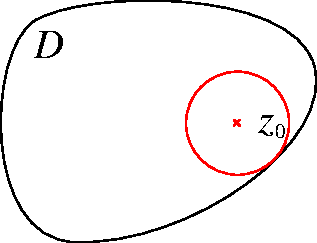
\includegraphics{maxdisk.pdf}
  \caption{$z_0$を中心として$D$の中にとれる最大の円板。}
  \label{fig:maxdisk}
\end{figure}


大事なことは、こういう微分が存在するというのは、\strong{非常に特別なこと}だということです。例えば実関数では、たとえ無限回微分可能であっても、解析的でないものが存在します。このような例を知っておくのは有用でしょう。次のような関数$f(x)$を考えましょう。
\begin{align}
  f(x)=
  \begin{cases}
    e^{-\frac{1}{x}}& (x>0)\\
    0&(x\le 0)
  \end{cases}.\label{examplenonanalytic}
\end{align}
この$f(x)$は$x=0$で何回でも微分可能です。実際$f^{(n)}(0)=0$となります。なので$f(x)$を$x=0$のまわりでTaylor展開してみたものは和が収束して
\begin{align}
  \sum_{n=0}^{\infty}\frac{f^{(n)}(0)}{n!}x^n=0
\end{align}
となります。しかし、これは$x>0$ではどんなに$x$が$0$に近くても$f(x)$とは異なります。したがって$f(x)$は$x=0$付近では、べき級数で表せません。

もしかしたら
「\eqref{examplenonanalytic}のような関数は無理やり手で作った変な関数で、数学では反例として重要かもしれないけど、物理では現れない。物理で現れる関数は解析的だ。」
と思うかもしれません。\strong{実は物理でも、このような非解析性が現れる場面があります。}例えば、量子力学でトンネル効果を考えたときの振幅は、$\hbar$が(特徴的な作用$S$に比べて)十分小さいとき近似的に
\begin{align}
  \sim e^{-\frac{S}{\hbar}}
\end{align}
のように表せます。これは先程の関数と同じ振る舞いですね。つまりこの量は$\hbar/S$が小さいとき、どんな$(\hbar/S)^n$よりも小さい量です。物理では$\hbar$のべき級数で表されるような補正を\strong{摂動論的な量子補正}
といいます。一方でべき級数で表されないような補正を\strong{非摂動論的な量子補正}と呼んでいます。トンネル効果は典型的な非摂動論的な量子補正です。

\section{解析接続}
$f(z)$を領域$D$で正則な関数とします。式\eqref{powerseries}は、「少なくとも」$z_0$を中心として$D$の中に収まる最大の円板の中で収束して成り立ちます。しかし場合によっては、式\eqref{powerseries}の右辺は、図\ref{fig:largerdisk}のように$D$をはみ出すような大きな円板$D'$の中でも収束するかもしれません。この場合、この$D'$が$D$からはみ出た部分では$f(z)$を式\eqref{powerseries}で「定義」することにより、大きな領域$D''=D\cup D'$の中で定義された正則関数$f(z)$を得ることができます。この操作を繰り返すことによって正則関数の定義域を広げていくことを\strong{解析接続}と呼びます。
\begin{figure}[htbp]
  \centering
  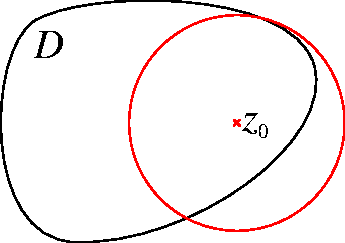
\includegraphics{largerdisk.pdf}
  \caption{$z_0$中心のTaylor展開が$D$をはみ出すような大きな円板で収束すれば、その収束する領域まで解析接続できる。}
  \label{fig:largerdisk}
\end{figure}


解析接続で定義域を広げるやり方は、「だいたい一意」であることを示す定理が次の「一致の定理」です。
\begin{theor}{一致の定理}{}
  領域$D$で正則な二つの関数$f(z),g(z)$があり、次の性質を満たしているとする。
  \begin{align*}
    \exists a \in D \text{ に収束する、ある点列 }z_n\in D,\ (n=1,2,3,\dots),\ z_n\ne a\text{ が存在し、}\nonumber\\
    f(z_n)=g(z_n),\ (n=1,2,3,\cdots)\text{を満たす。}
  \end{align*}
  すると、領域$D$で$f(z)=g(z)$である。
\end{theor}
この形が、仮定が最小で一番強いものですが、解析接続と直接関係があるのは、次の系です。
\begin{col}{}{}
  領域$D$で正則な二つの関数$f(z),g(z)$があり、次の性質を満たしているとする。
  \begin{align*}
    部分領域\exists D'\subset Dで f(z)=g(z)
  \end{align*}
  すると、領域$D$で$f(z)=g(z)$である。
\end{col}
つまり、いろんな解析接続のやり方で定義域を広げていって\strong{同じ領域まで広がったとすると}、いろんなやり方で解析接続した関数はすべて等しくなります。

さて、ややこしいところなのですが、この定理は、異なる領域に解析接続した場合には、何も言っていないことに注意してください。例えば、$D'$で正則な関数$f(z)$を$D_1\supset D'$と$D_2\supset D'$に解析接続した関数をそれぞれ$f_1(z), f_2(z)$とした場合、$D_1\cap D_2$で$f_1(z)=f_2(z)$\strong{とは限らない}ことに注意してください。このような例を後で紹介します。

次の一致の定理の系も使い勝手のよいものです。
\begin{col}{}{identity2}
  $N$個の関数$f_1(z),f_2(z),\dots,f_N(z)$は、領域$D$で正則であるとする。この中には、微分を含んでいてもよい。つまり$f_2(z)=f_1'(z)$のようなものでもよい。これらの関数が多項式の関係式
  \begin{align}
    F(f_1(z),f_2(z),\dots,f_N(z))=0,\label{polynomialrelation}
  \end{align}
  を部分領域$\exists D'\subset D$で満たしていたとする。
  すると、領域$D$でも関係式\eqref{polynomialrelation}を満たす。
\end{col}
特に、「正則な」微分方程式の解は解析接続しても、同じ微分方程式の解になっています。このことは後ほど
第\ref{sec:ode}章で微分方程式を取り扱うときに利用します。また、この定理は実際に解析接続を計算する際に実用的な手段を提供します。

解析接続の例をやってみましょう。
\begin{align}
  f(z)=\sum_{k=1}^{\infty}\frac{1}{k}z^k
\end{align}
という無限級数で表される関数を考えます。これはとりあえず領域$D'=\{z\in \Cb|\ |z|<1\}$で収束して正則関数になります。この$f(z)$を解析接続することを考えましょう。天下り的ですが、微分を考えてみます。項別微分して
\begin{align}
  f'(z)=\sum_{k=1}^{\infty}z^{k-1}
\end{align}
となります。次のような計算をしてみます。
\begin{align*}
  f'(z)-zf'(z)
  &=\sum_{k=1}^{\infty}z^{k-1}-\sum_{k=1}^{\infty}z^{k}\\
  &=(1+z+z^2+z^3+\dots)-(z+z^2+z^3+\dots)\\
  &=1
\end{align*}
となります。したがって関係式
\begin{align}
  (1-z)f'(z)-1=0\label{egrelation}
\end{align}
が$D'$で成り立つことが分かります。系\ref{:identity2}から、$f(z)$(あるいは$f'(z)$)を解析接続できたとしたら、その領域内すべてで\eqref{egrelation}が成り立つということが言えます。つまり解析接続できる限りにおいて
\begin{align}
  f'(z)=\frac{1}{1-z}
\end{align}
が成り立ちます。右辺は$z=1$を除く複素平面上で正則な関数なので$f'(z)$は$z=1$を除く複素平面上に解析接続できたことになります。この場合の$z=1$のように解析接続で絶対に正則に出来ないような点を$f'(z)$の\strong{特異点}と呼びます。

さて、$f'(z)$は出来る最大のところまで解析接続できたので、$f(z)$の解析接続を考えましょう。まず、$D'$に限ることにすると$f(0)=0$に注意すると
\begin{align}
  f(z)=\int_0^{z}f'(\zeta)d\zeta=\int_0^{z}\frac{d\zeta}{1-\zeta}\label{logintegralrep}
\end{align}
と書くことができます。ここで注意しないといけないのは、まず上の積分は2次元面内の線積分ですから、積分経路を指定しないといけません。しかし、$D'$内に限ると、任意の2つの経路は連続変形でつながりますから、Cauchyの積分定理により、経路によらないことが言えます(図\ref{fig:regionlog}を参照)。
\begin{figure}[htbp]
  \centering
  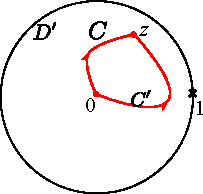
\includegraphics{regionlog.pdf}
  \caption{円板領域$D'$に限れば、どのような経路をとっても積分の値は変わらない。}
  \label{fig:regionlog}
\end{figure}
もし、式\eqref{logintegralrep}を$D'$の外側に拡張しようとすると、どのような不都合が起こるでしょうか?図\ref{fig:multivalue}を見てください。今度は、先程と異なり、連続変形ではつながらない経路が存在します。図\ref{fig:multivalue}の$C,C'$で実際積分の差を計算してみると留数計算を用いて
\begin{align}
  \int_{C}\frac{d\zeta}{1-\zeta}-\int_{C'}\frac{d\zeta}{1-\zeta}=\int_{C-C'}\frac{d\zeta}{1-\zeta}
  =2\pi i
\end{align}
となり、$2\pi i$だけ異なります。他に特異点$1$のまわりを何回もまわるような経路を考えると、一般に$2\pi i$の整数倍の不定性が存在することになります。
\begin{figure}[htbp]
  \centering
  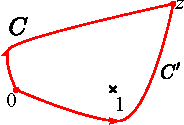
\includegraphics{multivalue.pdf}
  \caption{積分経路を$C$にするか$C'$にするかによって、積分の値が変わる。}
  \label{fig:multivalue}
\end{figure}

この不定性についての考え方はいくつかあります。一つの方法は$z=1$を除く$\Cb$全体に解析接続することを諦めて、少し小さな領域に限ることです。例えば、図\ref{fig:cut}のように、実軸上$z\ge 1$の半直線を定義域から抜く領域を考えます。このように関数の不定性をどうにかする場合に除く線状の集合を\strong{カット}と呼びます。また、カットの端の点を\strong{分岐点}と呼びます。このようにカットを入れた場合、図\ref{fig:multivalue}の$C'$の経路はありえません。実際図\ref{fig:cut}のようにカットを入れた領域では、$0$と$z$を結ぶ任意の経路は必ず連続変形でつながります。なので式\eqref{logintegralrep}で$f(z)$を表したものが解析接続になります。こうして作った$f(z)$は実軸上$z\ge 1$で実際不連続になります。先程の結果を用いると$x>1$として
\begin{align}
  f(x+i0)-f(x-i0):=\lim_{\epsilon\to +0}\qty(
    f(x+i\epsilon)-f(x-i\epsilon)
  )=2\pi i
\end{align}
となります。
\begin{figure}[htbp]
  \centering
  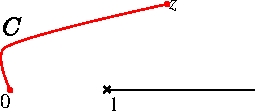
\includegraphics{cut.pdf}
  \caption{カットを入れた領域。$0$と$z$をつなぐ任意の経路は連続変形でつながる。}
  \label{fig:cut}
\end{figure}

上で挙げた不定性についての考え方のもう一つは、ワイエルシュトラスによる関数の概念の拡張です。上で説明したカットを入れて定義域を狭めてしまう方法は、ある意味非常にもったいないです。なので、不定性をもつことは諦めて、いけるところまでとことん解析接続することを考えます。こうしてしまうと、もともとの「関数」の定義であった、定義域内の1つの複素数に対して1つの複素数を対応させるというものから離れてしまい、定義域内の1つの複素数に対して、たくさんの複素数が対応してしまうものを考えることになります。このようなものを一般に\strong{多価関数}と呼びます。多価関数になることを厭わず、いけるところまで解析接続したものをすべて考えたものを\strong{ワイエルシュトラスの解析関数}と呼びます。例えば、先程の例をWeierstrassの解析関数と考えることができて
\begin{align}
  f(z)=-\log(1-z)
\end{align}
と書くことが出来ます。これは多価関数です。

\strong{リーマン面}はこの不定性に関する、また別の考え方です。多価関数になるのが嫌なので、定義域の方の概念を拡張してやることです。
例えば、図\ref{fig:cut}のようにカットを入れて考えた場合、下から解析接続してきたものと上から解析接続してきたものが不連続になってケンカしないようにカットのところで領地を分けています。ケンカしないもう一つの方法は、下から来た人と上から来た人に別々の領地をあてがってやることです。
図\ref{fig:riemannsurface}のように下から解析接続してきたものが、さらに解析接続していけるように別の\strong{シート}を用意してカットの下側とつなぎます。それとは別に上から解析接続してきたものがつながるシートも用意し、カットの上側とつなぎます。これをくりかえして、出来る限り解析接続していきます。
このようにしてシートをつないだ全体を\strong{リーマン面}と呼びます。解析接続したものはリーマン面上の一価関数になります。
\begin{figure}[htbp]
  \centering
  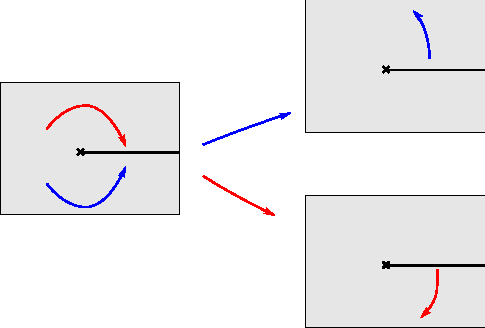
\includegraphics{riemannsurface.pdf}
  \caption{}
  \label{fig:riemannsurface}
\end{figure}

\section{多価関数、カット、ブランチ、……についての補足}
解析接続や多価関数、ブランチといった概念は馴染みにくく難しく思えるかもしれません。ただ、こういうものは実際の計算などにおいても有用なので、補足しておきます。

唐突ですが、$\sqrt{4}$はいくつでしょうか?$\sqrt{4}=2$ですよね。$\sqrt{4}=-2$と思う人はいませんね。なぜかというと、$x$が正の実数のとき、$\sqrt{x}$は2乗して$x$になるもののうち、正のものというふうに定義したからです。ここに不定性はありません。きっと高校までの数学では$\sqrt{\ }$の中に負の数や複素数は、入れないことにしていたと思います。こうしている限り平和です。

しかし、この講義で説明しようとしていることは、$\sqrt{\ }$の中に負の数や複素数を入れようとするとどうなるか、ということです。つまり
\begin{myquote}
  $\sqrt{-4}$はいくつか?
\end{myquote}
という問題を考えようとしています。これは、2乗して$-4$になる数でしょうから、二つの候補があります。
\begin{myquote}
  ① $\sqrt{-4}=2i$,\qquad ② $\sqrt{-4}=-2i$
\end{myquote}
の二つです。どちらが正解でしょうか。どちらも正の数ではありませんから昔の$\sqrt{\ }$の定義である「正のもの」は使えないことに注意してください。例えば①を支持する人は、次のような計算を使って説明するかもしれません。$\sqrt{-1}=i$を$i$の「定義」ということにして
\begin{align}
  \sqrt{-4}=\sqrt{-1}\sqrt{4}=2i
\end{align}
となりそうです。しかしちょっと待ってください。次のような計算も成り立ちそうです。
\begin{align}
  \sqrt{-4}=\sqrt{\frac{4}{-1}}=\frac{\sqrt{4}}{\sqrt{-1}}=-2i
\end{align}
となります。なので同じ理由で②ももっともらしいです。別の言い方をするなら
$f(z)=\sqrt{z}$という「関数」があったとき$f(-4)$はいくつか?ということになります。実は答えは
\begin{myquote}
  どういうカットを入れて、どういうブランチをとるかによっている。
\end{myquote}
というものです。

もう少し説明します。少し一般化して$f(z)=z^{\alpha}$という関数を考えましょう。$\alpha$は複素数の定数です。$\alpha=\frac12$の場合が先程の例になります。とりあえず、
\begin{align}
  f(z)=z^{\alpha}=\exp(\alpha\log z)\label{powerfunction}
\end{align}
という変形はできそうです。こう書いてみると少し前に出てきた$\log$がヤバイやつで元凶であることが見て取れます。一方で定数$\alpha$を掛けるとか、$\exp$とかはちゃんとした一価関数です。

実際に計算するためには、適当にカットを入れ、特定の\strong{分枝}(\strong{ブランチ}ともいう。多価関数の特定の値)を持ってくるのが便利なことが多いです。場面に応じて便利なとり方があるので、こうしなければならないという決まった取り方はありません。逆に言えば、問題や文脈ごとにカットやブランチが設定してあったりするのでよく読んでください。あるいは、自分で便利なように設定する必要がある場合もあります。

\eqref{powerfunction}の場合、一つの可能な取り方は次のようなものです。まず、実軸正の部分では高校でならった対数関数と同じにします。これを複素数も引数にとれる$\log$と区別して$\ln$と書くことにします\footnote{このような記号の使い分けは一般的ではありません。この講義の中だけでの使い分けです。}。つまり、$x>0$の場合
\begin{align}
  \log x=\ln x
\end{align}
としておきます。そして、図\ref{fig:cutrealnegative}のように、実軸負の部分にカットを入れることにします。\eqref{powerfunction}は複素平面から、この実軸負の部分のカットを除いた領域で正則関数になります。
\begin{figure}[htbp]
  \centering
  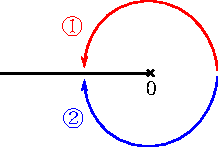
\includegraphics{cutrealnegative.pdf}
  \caption{}
  \label{fig:cutrealnegative}
\end{figure}

試しに、このカットでの不連続性を求めてみましょう。$x<0$として、カットに上から近づいた値$f(x+i0):=\lim_{\epsilon\to +0}f(x+i\epsilon)$を得るためには、図\ref{fig:cutrealnegative}の①のように実軸正の部分から解析接続していけばよいことになります。実際の計算は、$z=|x|e^{i\theta}$として、$\theta$を$0$から連続的に動かしていって$\theta\to\pi$の極限をとればよいことになります。つまり
\begin{align}
  f(x+i0)
  =\lim_{\theta\to \pi -0} \exp(\alpha \log |x|e^{i\theta})
  =\lim_{\theta\to \pi -0} \exp(\alpha \log |x|+\alpha i\theta)
  =\exp(\alpha\ln|x|+i\pi \alpha)
\end{align}
と計算できます。$\ln$は高校で習った対数関数、つまり中身は正の実数しか入れなくて、値は実数になる関数ですから、最後の表式には不定性は全く無いことに注意してください。同様にカットに下から近づいた値$f(x-i0):=\lim_{\epsilon\to +0}f(x-i\epsilon)$を求めるには図\ref{fig:cutrealnegative}の②のように解析接続すればよく、実際の計算は上で$\theta\to -\pi+0$の極限をとればよいことになりますから
\begin{align}
  f(x-i0)=\exp(\alpha\ln|x|-i\pi \alpha)
\end{align}
となります。前の問題に戻ると、このようなブランチをとった場合には、$\sqrt{-4+i0}=2i,\quad\sqrt{-4-i0}=-2i$となります。

別のカットの入れ方、ブランチの取り方もあります。カットは図\ref{fig:cutrealpositive}のように実軸正の部分に入れます。そして、$x>0$に対して
\begin{align}
  \log(x+i0)=\ln x \label{cutrealpositivebranch}
\end{align}
となるようなブランチをとります。この場合、前の問題は$\sqrt{-4}=2i$となります。カットのところでの不連続性を求めるのは、図\ref{fig:cutrealpositive}の赤い線に沿って前と同じように考えればできます。これは演習問題に残しておきます。
\begin{figure}[htbp]
  \centering
  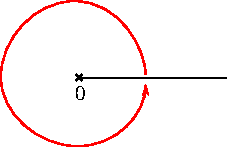
\includegraphics{cutrealpositive.pdf}
  \caption{}
  \label{fig:cutrealpositive}
\end{figure}

特殊関数を表すのに、カットの入った関数の積分を用いると非常に便利なことが多いのです。この手の積分を評価するのに与えられたブランチで留数を評価したり、カットでの不連続性を求めたりする必要がありますので、いろいろ演習問題をやってみて出来るようにしておいてください。

\section{孤立特異点}
孤立特異点については、数理物理2の授業でわりと詳しくやったことと思います。ここでは、言葉の復習だけをします。

領域$\widetilde{D}$とその中の点$z_0\in \widetilde{D}$があり、関数$f(z)$が$D=\widetilde{D}\setminus \{z_0\}$で正則のとき、$z_0$は$f(z)$の\strong{孤立特異点}であるといいます。

孤立特異点に関する最も重要な定理は、次のものです。
\begin{theor}{}{}
  $z_0$が$f(z)$の孤立特異点であるとき、$f(z)$は$z_0$のある近傍でローラン級数
  \begin{align}
    f(z)=\sum_{n=-\infty}^{\infty}a_n (z-z_0)^n \label{Laurentexpansion}
  \end{align}
  で表せる。具体的には$z_0$を中心として$\widetilde{D}=D\cup \{z_0\}$内でとれる最大の円板の半径を$r$としたとき、$0<|z-z_0|<r$で右辺の級数は収束し、等号が成り立つ。
\end{theor}

いくつかの言葉を導入します。
\begin{itemize}
  \item 式\eqref{Laurentexpansion}のような級数で表すことを\strong{ローラン展開}と呼びます。
  \item ローラン展開の式\eqref{Laurentexpansion}の負ベキの部分$\sum_{n=-\infty}^{-1}a_n(z-z_0)^n$を\strong{主要部}と呼びます。
  \item 主要部が$0$の場合、\strong{除去可能な特異点}あるいは\strong{正則点}と呼びます。除去可能な特異点は解析接続により、その点も含めて正則関数にできます。今後除去可能な特異点は除去して考えることにします。
  \item 主要部が有限項になる場合、この特異点は\strong{極}(pole)であるといいます。詳しく言うと、正の整数$k$に対して$a_{-k}\ne 0$で$a_n=0,\ n<-k$となっているとき、つまり一番特異的な項が$a_{-k}(z-z_0)^{-k}$であるときには、\strong{$k$位の極}といいます。
  \item 主要部が無限項からなる場合、この特異点は\strong{真性特異点}(essential singularity)であるといいます。
  \item $a_{-1}$のことを、この特異点の\strong{留数}(residue)と呼び
  \begin{align}
    a_{-1}=\Resi_{z=z_0}f(z)
  \end{align}
  と書きます。
\end{itemize}

「留数」にわざわざ大げさな名前がついているのは、この数が積分の評価に重要な役割を果たすからです。
\begin{theor}{}{}
  図\ref{fig:residue}のように閉じた反時計回りの経路$C$を考えます。関数$f(z)$は、$C$を含む領域で正則な関数とします。さらに$C$の内側では、特異点$z_1,z_2,\dots,z_N$を除いて$f(z)$は正則であるとします。このとき
  \begin{align}
    \oint_{C}f(z)\dd{z}=2\pi i\sum_{j=1}^{N}\Resi_{z=z_j}f(z)
  \end{align}
  が成り立ちます。
\end{theor}
\begin{figure}[htbp]
  \centering
  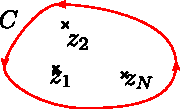
\includegraphics{residue.pdf}
  \caption{}
  \label{fig:residue}
\end{figure}


\section{リーマン球面}\label{sec:riemannsphere}
複素平面$\Cb$に一点$\infty$を付け加えたもの
\begin{align}
  \CP^1=\Cb\cup \{\infty\}
\end{align}
のことを\strong{リーマン球面}と呼びます。ここで、この$\infty$を「どこに付け加えるか?」について少し説明が必要です。また、これがなぜ「球面」と呼ばれるのかについても説明します。

まずは、「どこに付け加えるか?」というのはどういう意味か?ということについて説明します。これは、\strong{位相}(\strong{トポロジー})と呼ばれる構造を決めることです。みなさんの中でトポロジーに馴染みのある方は少ないでしょうから、だいたいの説明をします。
トポロジーを決めるとは、極限とか収束とかをどうするかを決めることです。複素平面内のある点$c$に近づいていく数列$\{a_n\}_{n=1}^{\infty}$があったら、その数列は$c$に収束するといいます。
しかし、例えば$\lim_{n\to \infty}|a_n|=\infty$となる数列だったら、その数列は複素平面内のどの点にも近づかないですから、「発散する」としか言いようがないです。
しかし気持ち的に「$\infty$に近づく」あるいは「$\infty$に収束する」と言いたくならないですか?複素平面内には$\infty$という点はありませんから、複素平面内にこだわる限りこういう言い方はできません。こういうことがあるので複素平面に$\infty$を付け加えたリーマン球面を考えることが便利なのです。リーマン球面の中で考えるなら「$\infty$に収束する」という言いかたが出来ます。この意味で先程の「どこに付け加えるか?」という問いに対する一つの答えは「$\lim_{n\to\infty}|a_n|=\infty$となる数列の行き先」と言うことができます。

別の説明をします。$\Cb$を平面という幾何学的な対象だと思って、複素数$z$をその座標と思うことにします。この同じ平面を別の座標で考える、つまり座標変換を考えます。$z$と
\begin{align}
  w=\frac{1}{z}\label{inversion}
\end{align}
という関係がある$w$を考えましょう。$w$は$z=0$の点はうまく表すことが出来ませんが、それ以外の$\Cb$の点はうまく表すことができます。リーマン球面$\CP^1$にするとどうでしょうか。$\infty$という一点を付け加えるわけですが、この$\infty$は無限ですから$z$という座標ではうまく表せません。しかし、$w$でいうと$w=0$が、この新しく付け加えた$\infty$です。$0$はれっきとした複素数なので$w$という座標で考える限り、この点は他の点と大差なく考えることができます。

式\eqref{inversion}は次のような非常に良い性質を持っているので、$\infty$を取り扱う実用的な方法として優れています。式\eqref{inversion}は$z=0$を除いた領域で($\CP^1$上でいうなら$\infty$も除いて)正則関数になっています。なのでこの領域の部分領域での$z$の正則関数は$w$の正則関数になります。複素関数論で最も大事であった「正則関数」という概念が$z$で考えても$w$で考えても、$0$と$\infty$を除いて同じですので我々の目的には非常に都合がよいです。

もう一つ別の説明をします。これは、なぜリーマン「球面」と呼ばれるのかということも含めた説明です。図\ref{fig:riemannsphere}のように、複素平面上の点$z$と球面から北極を除いたものの上の点$P$を一対一に対応させることができます。図\ref{fig:riemannsphere}では、平面の上に南極が原点に接するように球面が置かれています。こうしておいて、北極と平面上の点$z$を結んだ直線と球面の交わる点を$P$とし、この点を$z$と対応させます。このような対応があるので、
\strong{複素平面$\Cb$と球面から北極を除いたものはトポロジーが同じ}ということができます\footnote{実はもっと強くて、「角度が同じ」まで言えます。正則関数とは角度を保つ関数でしたから、球面上の正則関数という概念があって、今の対応でそれは平面上の正則関数と同じということができます。}。
リーマン球面$\CP^1$は平面に一点を付け加えたものですが、さきほどの対応に加えて$\infty$を北極に対応させます。こうしておくと、平面上で絶対値がどんどん大きくなっていく点列に対応するものは、球面上で北極にどんどん近づいていく点列になります。ですので、これまで考えてきた$\infty$の付け加え方と同じになります。まとめると\strong{リーマン球面$\CP^1$と球面はトポロジーが同じ}ということができます。
\begin{figure}[htbp]
  \centering
  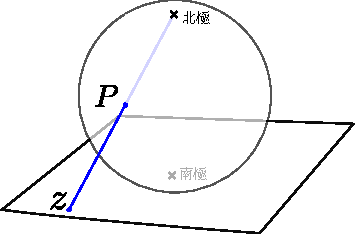
\includegraphics[width=8cm]{riemannsphere.pdf}
  \caption{}
  \label{fig:riemannsphere}
\end{figure}

\subsection{リーマン球面上の特異点}
少しだけ、言葉を導入します。領域$D$を$\Cb\setminus D$が有界となるものとします。$D$上の正則関数$f(z)$を考えます。このとき$g(w)=f(1/w)$において$w=0$が正則、極、真性特異点であるとき、$f(z)$は$z=\infty$でそれぞれ正則、極、真性特異点であるといいます。

次の定理は非常に強力な定理です。
\begin{theor}{リウビルの定理}{Liouville}
  $f(z)$が$\CP^1$上正則(つまり$\Cb$上正則かつ$z=\infty$でも正則)であるなら、$f(z)$は定数である。
\end{theor}
例えば、次のようなことが示せます。
\begin{col}{}{meromorphic}
  $f(z)$が$\CP^1$上で極を除いて正則である(有理型関数であるといいます)なら、$f(z)$は有理関数である。
\end{col}

これを証明してみましょう。まず、$\CP^1$上で極を除いて正則なら極の数は有限個です。なぜなら、もし無限個あったとしたら必ずどこかの点に集積していて\footnote{$\CP^1$がコンパクトであるということから従います。これも$\CP^1$を考えることの一つのメリットです。}その集積点は孤立特異点ですらなくなってしまい、極ではない特異点があるので仮定に反します。

次に$f(z)$の各特異点における主要部をすべて足したものを$g(z)$とします。特異点は、すべて極で有限個しかないので、$g(z)$は有限個の有理関数の和になるので、有理関数です。ここで
\begin{align}
  h(z)=f(z)-g(z)
\end{align}
を考えます。$f(z)$の各特異点まわりの主要部は、$g(z)$のそれと同じですから、$h(z)$は$\CP^1$上正則関数になります。したがって定理\ref{:Liouville}より$h(z)=c$(定数)となり、$f(z)=g(z)+c$となります。$g(z)$は有理関数ですから、$f(z)$も有理関数です。(証明終わり)

このことを踏まえると標語的に次のことが言えると思います。
\begin{myquote}
「面白い」関数は特異点を持っていて、その「面白さ」は特異点のところにつまっている。
\end{myquote}
この講義では様々な関数について勉強しますが、特に特異点に注目して調べるとよいということが分かります。中でも第\ref{sec:ode}章では、微分方程式をその特異点によって分類することにより、超幾何関数という新しくて有用なクラスの関数を得ることができます。

\subsection{メビウス変換}
次の定理は$\CP^1$の「座標変換」についてのものです。
\begin{theor}{}{}
次の2つは同値である
\begin{enumerate}
  \item $f(z)$は$\CP^1$から$\CP^1$への全単射で、$\infty$に行くところ以外では正則である。
  \item 
\begin{align}
  f(z)=\frac{az+b}{cz+d},\quad a,b,c,d:\ \text{定数}, ad-bc\ne 0\label{Moebius}
\end{align}
\end{enumerate}
\end{theor}
式\eqref{Moebius}で表されるような変換を\strong{一次分数変換}あるいは\strong{メビウス変換}と呼びます。メビウス変換に関して、特に重要な性質は、$\CP^1$上の任意の異なる3点が与えられたとき、それらをそれぞれ$0,1,\infty$にうつすようなメビウス変換が必ず存在することです。

\subsection{リーマン球面での積分}

積分を評価するときに留数というのは非常に重要でした。では、$\infty$での留数はどうなっているでしょうか。これを考えるときには、$f(z)\dd{z}$というかたまりで考えるとよいです。$\infty$を考えるときには、$w=1/z$と変数変換するのが便利でした。すると$\dd{z}=-\frac{1}{w^2}dw$ですから
\begin{align}
  f(z)\dd{z}=-f(1/w)\frac{dw}{w^2}
\end{align}
の$w=0$での留数を考えればよいです。

例をやってみましょう。
\begin{align}
  f(z)\dd{z}=\qty(\frac{1}{z}+\frac{1}{z+1})\dd{z}
\end{align}
とします。$z=1/w$とすると
\begin{align}
  f(z)\dd{z}=-\qty(w+\frac{1}{1/w+1})\frac{dw}{w^2}
  =\qty(-\frac{2}{w}+\frac{1}{w+1})dw
\end{align}
となります。なので
\begin{align}
  \Resi_{z=\infty}f(z)\dd{z}:=\Resi_{w=0}\qty(-f(1/w)\frac{dw}{w^2})=-2
\end{align}
となります。

これに関して面白い定理があります。
\begin{theor}{}{}
  $f(z)$は$\Cb\setminus\{z_1,\dots,z_N\}$で正則とする。このとき次が成り立つ。
  \begin{align}
    \sum_{j=1}^{N}\Resi_{z=z_j}f(z)\dd{z}+\Resi_{z=\infty}f(z)\dd{z}=0
  \end{align}
\end{theor}
証明の方針は、次の通りです。まずは内部に特異点を持たない小さな時計回りのループ$C$を考えるとコーシーの積分定理より$\oint_{C}f(z)\dd{z}=0$です。
このループを変形していってどんどん大きくしていくと、$\infty$も含めてすべての特異点のまわりを反時計回りに回るループの和になります(図\ref{fig:residuetheorem}参照)。なので
\begin{align}
  0=\oint_{C}f(z)\dd{z}=\sum_{j=1}^{N}\Resi_{z=z_j}f(z)\dd{z}+\Resi_{z=\infty}f(z)\dd{z}
\end{align}
となります。
\begin{figure}[htbp]
  \centering
  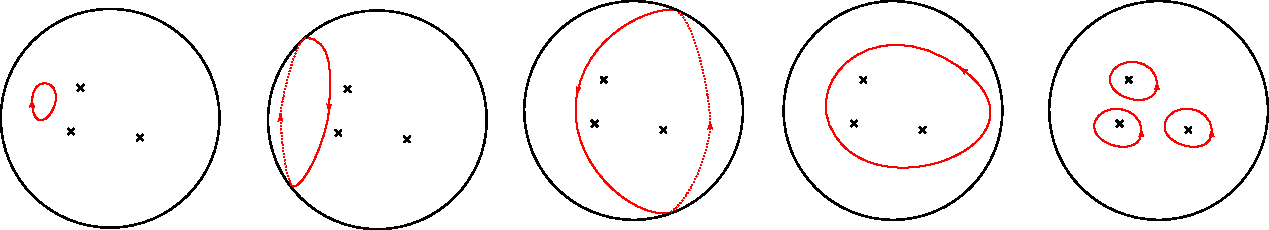
\includegraphics[width=14cm]{residuetheorem.pdf}
  \caption{経路の変形の様子。リーマン球面を球面で現している。}
  \label{fig:residuetheorem}
\end{figure}

\section{まとめ}
この章では、複素関数論についての復習と、少し新しいことをやりました。
\begin{itemize}
  \item 正則関数というのは、非常に特別な関数です。
  \item 正則性を保ったまま定義域を広げる「解析接続」という概念があります。
  \item 解析接続を考えると多価関数が現れることがよくあります。
  \item 多価関数を取り扱う1つの方法は、「カット」を入れて1つのブランチ(多価関数の値の1つ)をとってくることです。このカットでの不連続性の積分は、今後よく出てきます。
  \item ワイエルシュトラスの解析関数やリーマン面といった新しい概念が出てきます。
  \item 複素平面に$\infty$を付け加えた「リーマン球面」は便利な概念です。
  \item 関数を調べる際には「特異点」を調べるのが重要です。
\end{itemize}


\chapter{ガンマ関数とその周辺}
特殊関数の中で最もよく物理に現れるのがガンマ関数です。この節では、このガンマ関数について様々な性質を見ていきます。
\section{定義など}
ここでは、次のように定義します。
\begin{definition}{ガンマ関数}{gammafunction}
\begin{align}
  \Gamma(z)=\int_0^{\infty}dt t^{z-1}e^{-t}\label{eulerintegral}
\end{align}
の右辺の積分が絶対収束するような$z$に関してガンマ関数$\Gamma(z)$をこの式で定義する。解析接続により、できる限り定義域を広げる。
\end{definition}

まず、積分が絶対収束する範囲を考えてみましょう。発散する危険性を考えなければならないのは、$t\to\infty$と$t\to 0$です。$t\to\infty$は$e^{-t}$が非常に速く$0$に近づくので、どんな$z$に対しても収束します。$t\to 0$の部分を考えましょう。このとき$e^{-t}$は$1$としてよいです。絶対値の積分は$\Re z\ne 0$の場合
\begin{align}
  \lim_{\epsilon\to 0}\int_{\epsilon}^{a}dt t^{\Re z-1}=\lim_{\epsilon\to 0}(-\frac{1}{\Re z}\epsilon^{\Re z}+(\text{有限}) )
\end{align}
となりますので、$\Re z>0$のとき絶対収束します。

ガンマ関数に関して、最も重要な公式は、次のものです。
\begin{important}
  \begin{align}
    \Gamma(z+1)=z\Gamma(z)\label{gammaformula}
  \end{align}
\end{important}
証明は次のとおりです。$\Re z >0$のとき、
\begin{align}
  \Gamma(z)
  =\int_0^{\infty}dt t^{z-1}e^{-t}
  =\int_0^{\infty}dt \frac{1}{z}\dv{t}(t^{z})e^{-t}
  =\int_0^{\infty}dt \frac{1}{z}\qty[\dv{t}(t^{z}e^{-t})+t^ze^{-t}],\\
\Rightarrow
z\Gamma(z)=[t^{z}e^{-t}]_0^{\infty}+\int_0^{\infty}dt t^{z}e^{-t}=\Gamma(z+1)
\end{align}
となるので、\eqref{gammaformula}が成り立ちます。その他の領域では、解析接続で定義されるので、一致の定理の系\ref{:identity2}より、\eqref{gammaformula}が成り立ちます。(証明終わり)

いろんな点での値を求めてみましょう。まずは
\begin{align}
  \Gamma(1)=\int_{0}^{\infty} dt e^{-t}=1
\end{align}
はすぐに計算できます。ここから$n$を$0$以上の整数として
\eqref{gammaformula}を何回も用いると
\begin{align}
  \Gamma(n+1)=n\Gamma(n)=n(n-1)\Gamma(n-1)=\dots
  =n(n-1)\dots 2\cdot 1 \Gamma(1)=n!
\end{align}
と計算できます。なので
\begin{important}
\begin{align}
  \Gamma(n+1)=n!  \label{gammafactorial}
\end{align}
\end{important}
という結果を得ました。つまり、ガンマ関数は階乗を正の整数以外に拡張したものということができます。

もう一つ値を簡単に求めることができるのは$\Gamma(1/2)$です。ガウス積分を変形していって
\begin{align}
  \sqrt{\pi}&=\int_{-\infty}^{\infty}\dd{x}e^{-x^2}
  =2\int_{0}^{\infty}\dd{x}e^{-x^2}\nonumber\\
&=\int_{0}^{\infty}\dd{t} t^{-\frac12}e^{-t}=\Gamma\qty(\frac12)
\end{align}
となります。ここで一行目から二行目に行くときは$t=x^2$という積分変数の変換を行いました。得られた公式は
\begin{important}
  \begin{align}
    \Gamma\qty(\frac12)=\sqrt{\pi}
  \end{align}
\end{important}
となります。ここからさらに公式\eqref{gammaformula}を用いることにより、$\Gamma\qty(\frac12 +n),\ (n\in \Zb)$の値を得ることができます。

\section{解析接続}
定義\ref{:gammafunction}では、解析接続を含んでいました。ここでは、具体的にこの解析接続がどこまで行けるのかを詳しく見てみましょう。使う公式は\eqref{gammaformula}です。これは関数等式ですから、一致の定理の系\ref{:identity2}より、解析接続しても成り立ちます。これを何回も用いることにより
\begin{align}
  \Gamma(z)=\frac{1}{z}\Gamma(z+1)=\frac{1}{z(z+1)}\Gamma(z+2)=\dots
  =\frac{1}{z(z+1)\dots(z+n)} \Gamma(z+n+1)\label{gammaproduct1}
\end{align}
と変形できます。一番最後の表式は、$\Re z > -n-1,\ z\ne 0,-1,-2,\dots,-n$で正則であることが、分かります。
$n$は好きなだけ大きくとれることも考え合わせると次のことが言えます。
\begin{important}
  $\Gamma(z)$は、$\Cb\setminus \{0,-1,-2,-3,\cdots\}$で正則である。
\end{important}

$n=0,1,2,3,\cdots$として、$\Gamma(z+n+1)$は$z=-n$の近傍で正則ですから、\eqref{gammaproduct1}から$z=-n$は\strong{1位の極である}ことが分かります。さらにその留数は
\begin{align}
  \lim_{z\to -n}(z+n)\Gamma(z)=\frac{1}{(-n)(-n+1)\dots(-1)}\Gamma(1)
  =(-1)^n \frac{1}{n!}
\end{align}
と計算できるので
\begin{align}
  \Resi_{z=-n}\Gamma(z)=(-1)^n \frac{1}{n!}
\end{align}
であることが分かります。

\section{スターリングの公式}
次に、ガンマ関数の近似式であるスターリングの公式について説明します。ここでは、鞍点法と呼ばれる物理において非常に有用な近似方法について、まず説明します。それから、その応用例の一つとしてスターリングの公式を説明します。

\subsection{鞍点法}

\begin{figure}[htbp]
  \centering
  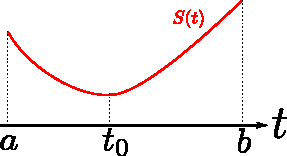
\includegraphics{saddlefunction.pdf}
  \caption{}
  \label{fig:saddlefunction}
\end{figure}
次のような積分を考えましょう。$N$を正の実数として
\begin{align}
  f(N):=\int_{a}^{b}A(t)e^{-N S(t)}dt.\label{saddleintegral}
\end{align}
ここで$A(t)$と$S(t)$は$N$によらない$t$の関数とします。$S(t)$は、$t=t_0\ (a<t_0<b)$で最小値をとり、この近傍で2階微分可能で、しかも$S''(t)>0$であるとします。図\ref{fig:saddlefunction}のような図を思い浮かべてください。

式\eqref{saddleintegral}の積分を$N$が非常に大きいときに近似的に評価することを考えましょう。

式\eqref{saddleintegral}の積分は
\begin{align}
  f(N)=e^{-NS(t_0)}\int_{a}^{b}A(t)e^{-N (S(t)-S(t_0))}dt\label{saddleintegral2}
\end{align}
と書き換えられます。ここで積分の中にある関数$g(t):=e^{-N (S(t)-S(t_0))}$について考えてみましょう。
まず、$g(t_0)=1$です。
そして$S(t_0)$は$S(t)$の最小値ですから、$t\ne t_0$で$S(t)-S(t_0)>0$です。
なので$N$が非常に大きいとき$t\ne t_0$では、$g(t)$はほとんど$0$になります。
つまり、$g(t)$は図\ref{fig:saddlefunction2}のように$t=t_0$に鋭いピークを持ち、それ以外のところでは、ほとんど$0$になります。
ですから\strong{積分を評価するときに$t=t_0$付近のみ考えても良い近似が得られる}ということになります。
\begin{figure}[htbp]
  \centering
  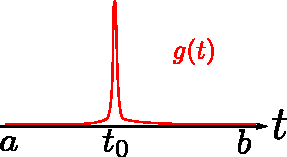
\includegraphics{saddlefunction2.pdf}
  \caption{}
  \label{fig:saddlefunction2}
\end{figure}

さて\eqref{saddleintegral2}の積分を$t=t_0$付近だけで近似することを考えましょう。このために$S(t)$を$t=t_0$まわりでTaylor展開します。$t=t_0$で最小値ですから$S'(t_0)=0$です。ですから
\begin{align}
  S(t)-S(t_0)=\frac12 S''(t_0) (t-t_0)^2+O((t-t_0)^3)
\end{align}
となります。式の簡単のために変数$\tau=t-t_0$を導入します。また、積分範囲は、もともと$a$から$b$まででしたが、$t=t_0$付近以外の寄与は小さいので$-\infty$から$\infty$に変えてもよい近似になります。また、$A(t)$は$N$によってないので、$t$をピークの値である$t_0$に置き換えてしまいます。こうして$O(\tau^3)$を無視してガウス積分を実行すると\footnote{$S''(t_0)>0$という仮定を使っています。}
\begin{align}
  f(N)\cong e^{-NS(t_0)}\int_{-\infty}^{\infty}A(t_0)e^{-N\qty( \frac12 S''(t_0) \tau^2)}\dd{\tau}
  =e^{-NS(t_0)}A(t_0)\sqrt{\frac{2\pi}{NS''(t_0)}}
\end{align}
という近似を得ます。改めて書くと$N$が非常に大きいとき
\begin{important}
  \begin{align}
    \int_{a}^{b}A(t)e^{-N S(t)}\dd{t}=e^{-NS(t_0)}A(t_0)\sqrt{\frac{2\pi}{NS''(t_0)}}(1+O(N^{-1}))
  \end{align}
\end{important}
となります。誤差の項$O(N^{-1})$は、ここでは詳しく説明しませんが、補正項を求めにいくことで分かります。

\subsection{ガンマ関数と鞍点法}
さて$z$が正の実数で非常に大きい場合に$\Gamma(z)$を鞍点法で近似することを考えましょう\footnote{実際には$z$の虚部が少しくらいあっても適用できますが、ここでは簡単のために実数としておきます。}。

積分の形\eqref{eulerintegral}を用いて
\begin{align}
  \Gamma(z)
  =\int_{0}^{\infty}t^{z-1}e^{-t}\dd{t}
  =\int_{0}^{\infty}e^{-t}e^{(z-1)\ln t}\dd{t}\label{tempgamma}
\end{align}
と変形できるので、$S(t)=-\ln t$とすれば、式\eqref{saddleintegral}の形にかなり近い気がします。しかし、$-\ln t$には今の積分範囲の内点に最小値が無いので、これはうまくいきません。

そこで、次のような工夫をします。まず、式を見やすくするために$N=z-1$とおきます。そして$u=\frac{t}{N}$ という変数変換をします。すると式\eqref{tempgamma}は
\begin{align}
  \Gamma(z)
  =N\int_{0}^{\infty}\dd{u}e^{-Nu+N\ln(uN)}
  =Ne^{N\ln N}\int_{0}^{\infty}\dd{u}e^{-N(u-\ln u)}\label{tempgamma2}
\end{align}
と書けます。今度は$S(u)=u-\ln u$とすれば\eqref{saddleintegral}の形になりました。

これを前と同じように変形していきます。$S$を最小にする$u$を$u_0$とします。これは$S'(u_0)=0$を満たすはずです。$S'(u)=1-\frac{1}{u}$なので$u_0=1$と求まります。ここから$S(u_0)=1,\ S''(u_0)=1$が分かるので、$\tau=u-u_0$とおくことにより、\eqref{tempgamma2}は
\begin{align}
  \Gamma(z)=N^{N+1}\int_{-\infty}^{\infty}\dd{\tau}e^{-N}e^{-N\frac12 \tau^2+NO(\tau^3)}=N^{N+1}e^{-N}\sqrt{\frac{2\pi}{N}}(1+O(N^{-1}))
\end{align}
となります。$N=z-1$であったことを思い出すと\strong{スターリングの公式}
\begin{important}
  \begin{align}
    \Gamma(N+1)=N^{N}e^{-N}\sqrt{2\pi N}(1+O(N^{-1}))\label{starling}
  \end{align}
\end{important}
が得られます。特に$N$が正の整数のとき$\Gamma(N+1)=N!$でしたから
\begin{important}
  $N$が大きな正の整数のとき
\begin{align}
  N!=N^{N}e^{-N}\sqrt{2\pi N}(1+O(N^{-1}))\label{starling2}
\end{align}
\end{important}
という近似式が得られます。これは統計力学などで非常に有用な近似式です。

\section{ガンマ関数の様々な表示}
ガンマ関数は積分\eqref{eulerintegral}以外にも様々な表示の仕方があります。ここでは、そのうちのいくつかを見ていきましょう。
\subsection{積の極限による表示}
まずは、次のような極限による表示です。
\begin{important}
  \begin{align}
    \Gamma(z)=\lim_{n\to\infty}\frac{n!n^z}{z(z+1)\dots (z+n)}.
    \label{gammaproductlimit}
  \end{align}
\end{important}
教科書によっては、これをガンマ関数の定義としてあるものもあります。

証明は次のとおりです。アイデアは式\eqref{gammaproduct1}
\begin{align}
  \Gamma(z)=\frac{1}{z(z+1)\dots (z+n)}\Gamma(z+n+1)
  \label{gammaproduct1re}
\end{align}
において$\Gamma(z+n+1)$をスターリングの公式\eqref{starling}を用いて見積もってやることです。\eqref{starling}で$N=z+n$とすると
\begin{align}
  \Gamma(z+n+1)=(z+n)^{z+n}e^{-(z+n)}\sqrt{2\pi(z+n)}(1+O(n^{-1}))
  \label{tempgammaproduct1}
\end{align}
となります。ここではスターリングの公式は$N$に少しくらい虚部があってもよいことを証明なしで用いました\footnote{証明は積分経路の変形をして鞍点法を用いるだけなので、そんなに難しくありません。挑戦してみてください}。あと$z$は有限で$n$が非常に大きいので$(z+n)^{-1}=n^{-1}(1+O(n^{-1}))$であることも用いました。

式\eqref{tempgammaproduct1}をさらに評価するために
\begin{align}
  \sqrt{2\pi(n+z)}&=\sqrt{2\pi n}(1+O(n^{-1})),\\
  \qty(1+\frac{z}{n})^{z+n}&=e^{z}(1+O(n^{-1}))
\end{align}
という2つの事実を用います。上の式は簡単に示せます。下の式は両辺の$\ln$を比較すると示せます。これらを用いると式\eqref{tempgammaproduct1}から
\begin{align}
  \Gamma(z+n+1)=n^{z+n}\qty(1+\frac{z}{n})^{z+n}e^{-z}e^{-n}\sqrt{2\pi n}(1+O(n^{-1}))
  =n^n e^{-n}\sqrt{2\pi n}n^z(1+O(n^{-1}))
\end{align}
となります。ここでスターリングの公式\eqref{starling2}で$N=n$とすると$n!=n^ne^{-n}\sqrt{2\pi n}(1+O(n^{-1}))$を得るので、これを用いると
\begin{align}
  \Gamma(z+n+1)=n!n^z(1+O(n^{-1}))
\end{align}
と評価できます。

これを\eqref{gammaproduct1re}に代入して
\begin{align}
  \Gamma(z)=\frac{n!n^z}{z(z+1)\dots (z+n)} (1+O(n^{-1}))
\end{align}
を得ます。ここで$n\to\infty$の極限をとれば証明したかった式\eqref{gammaproductlimit}を得ます。


\subsection{無限積表示}
次は無限積表示です。
\begin{important}
  \begin{align}
    \Gamma(z)=\frac{1}{e^{\gamma z}z \prod_{k=1}^{\infty}\qty(1+\frac{z}{k})e^{-z/k} }.  \label{gammainfiniteproduct}  
  \end{align}
\end{important}
ここで$\gamma$は\strong{オイラー定数}と呼ばれる定数で
\begin{align}
  \gamma:=\lim_{n\to\infty}\qty(\sum_{k=1}^{n}\frac{1}{k}-\ln n)\label{defeulerconst}
\end{align}
で定義されます。この極限はちゃんと有限の値を持ち$\gamma=0.57721\dots$であることが知られています。

さて、\eqref{gammainfiniteproduct}を証明しましょう。使うのは、\eqref{gammaproductlimit}です。これは
\begin{align}
  \Gamma(z)=\lim_{n\to\infty}e^{z\ln n}\frac{1}{z}
  \prod_{k=1}^{n}\frac{k}{z+k}\label{tempgammainfiniteproduct}
\end{align}
と書き換えられます。積の部分をさらに変形して
\begin{align}
  \prod_{k=1}^{n}\frac{k}{z+k}=\prod_{k=1}^{n}\frac{1}{1+\frac{z}{k}}=\frac{\prod_{k=1}^{n}e^{-z/k}}{\prod_{k=1}^{n}\qty(1+\frac{z}{k})e^{-z/k}}
\end{align}
となります。最後の式の分母の$\prod_{k=1}^{n}\qty(1+\frac{z}{k})e^{-z/k}$が$n\to\infty$の極限で収束するところがミソです。これを式\eqref{tempgammainfiniteproduct}に戻してオイラー定数の定義\eqref{defeulerconst}を用いると
\begin{align}
  \Gamma(z)=\lim_{n\to\infty}e^{z\ln n-\sum_{k=1}^n z/k}\frac{1}{z}
  \frac{1}{\prod_{k=1}^{n}\qty(1+\frac{z}{k})e^{-z/k}}
  =\frac{1}{e^{\gamma z}z \prod_{k=1}^{\infty}\qty(1+\frac{z}{k})e^{-z/k} }
\end{align}
となって無限積表示\eqref{gammainfiniteproduct}を得ます。


\subsection{Hankelの積分表示}
\eqref{eulerintegral}の積分は$\Re z>0$のみで収束しましたが、うまく複素積分を使うと整数以外の複素数$z$で有効な積分を用いた表示を得ることができます。
\begin{important}
  \begin{align}
    \Gamma(z)=\frac{1}{e^{2\pi i z}-1}\int_{C}\dd{t}t^{z-1}e^{-t}.\label{hankelintegral}
  \end{align}
\end{important}
ここで積分経路$C$は図\ref{fig:hankel}のようにとります。$t^{z-1}=\exp((z-1)\log t)$は$t$の多価関数ですのでブランチを指定する必要があります。ブランチは$x>0$に対して$\log(x+i0)=\ln x$ (実数)ととります。式\eqref{cutrealpositivebranch}のあたりの議論を思い出してください。
\begin{figure}[htbp]
  \centering
  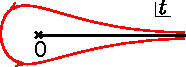
\includegraphics[width=5cm]{hankel.pdf}
  \caption{}
  \label{fig:hankel}
\end{figure}


証明をしましょう。まず、積分の部分
\begin{align}
  I=\int_{C}\dd{t}t^{z-1}e^{-t}
\end{align}
を見てみます。これは、任意の複素数$z$に対して収束する積分です。なぜなら積分経路上に特異点はなく、$t\to \infty$のところも$e^{-t}$のせいで被積分関数は十分速く$0$に近づくからです。さらに$I$は$z$で微分可能ですから$\Cb$上正則関数になります。ですから$\Re z>0$の場合に\eqref{hankelintegral}を示せば、一致の定理の系\ref{:identity2}により、整数でない複素数の$z$で式\eqref{hankelintegral}が成り立つことが言えます。

\begin{figure}[htbp]
  \centering
  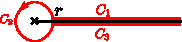
\includegraphics[width=5cm]{hankel2.pdf}
  \caption{経路を変形して3つに分ける。$C_1, \ C_3$はそれぞれ実軸上カットのすぐ上とすぐ下で$t\ge r$の部分。$C_2$は原点中心、半径$r$の円周。}
  \label{fig:hankel2}
\end{figure}
次に$\Re z>0$のときに、$I$の評価をします。このために、積分経路を変形し、カットでの不連続性の積分に直します。$C$を図\ref{fig:hankel2}のように3つの部分$C_1,\ C_2,\ C_3$に分けます。そして
\begin{align}
  I=I_1+I_2+I_3,\quad I_i=\int_{C_i}\dd{t}t^{z-1}e^{-t},\ (i=1,2,3)
\end{align}
として$I_1,I_2,I_3$のそれぞれを$r\to 0$で評価していきます。

まず、$I_2$からいきます。$I_2\to 0$であることを示します。次のような不等式を立てられます。
\begin{align}
  0\le |I_2|=\qty|\int_{C_2}\dd{t}t^{z-1}e^{-t}|\le
  \int_{C_2}\qty|\dd{t}t^{z-1}e^{-t}|
  \le \int_{C_2}\qty|\dd{t}t^{z-1}|e^{r}.
\end{align}
$t=re^{i\theta},\ z=x+iy$とおくと$|\dd{t}|=\dd{\theta}r,\ |t^{z-1}|=r^{x-1}e^{-\theta y}$となるので
\begin{align}
  0\le |I_2|
  \le \int_{0}^{2\pi}\dd{\theta} r^{x}e^{-\theta y}e^{r}.
  = r^{x}e^{r}\int_{0}^{2\pi}\dd{\theta} e^{-\theta y}\to 0\ (r\to 0)
\end{align}
となって$I_2\to 0$が示せます。最後のところで積分が残っていますが、この積分は$r$によらない定数であることに注意してください。また$x=\Re z>0$であることを用いました。

次に、$I_1,\ I_3$を評価します。複素関数としての被積分関数を$g(t)$とします。$s>0$として$g(s-i0)=e^{2\pi i z} g(s+i0)$なので
\begin{align}
  I_1+I_3=-\int_{0}^{\infty}\dd{s} g(s+i0)+\int_{0}^{\infty}\dd{s}g(s-i0)
  =(e^{2\pi iz}-1)\int_{0}^{\infty}\dd{s} g(s+i0)\nonumber\\
  =(e^{2\pi iz}-1)\int_{0}^{\infty}\dd{s} s^{z-1}e^{-s}
  =(e^{2\pi iz}-1)\Gamma(z)
\end{align}
を得ます。

合わせると、$z$が整数でない場合
\begin{align}
 \Gamma(z)=\frac{1}{e^{2\pi iz}-1} I
\end{align}
となって\eqref{hankelintegral}が示せました。


\section{ベータ関数}
ここでは、ガンマ関数と非常に関係が深い「ベータ関数」という関数を導入します。ベータ関数は実はガンマ関数で表すことができるので、ガンマ関数が完全に分かればベータ関数も分かることになります。しかし、ベータ関数としての性質を知っておくのも有用です。また物理では弦理論の散乱振幅にベータ関数が出てきます。

ここでは、ベータ関数を次のように定義します。
\begin{definition}{ベータ関数}{}
  $\Re u>0, \ \Re v >0$のとき$B(u,v)$を
  \begin{align}
    B(u,v)=\int_0^{1}\dd{x} x^{u-1}(1-x)^{v-1}\label{betaintegral}
  \end{align}
  で定義します。他の$u,v$にも出来る限り解析接続で定義します。
\end{definition}

定義からすぐ分かる公式があります。式\eqref{betaintegral}で$y=1-x$の変数変換をすることで
\begin{important}
  \begin{align}
    B(u,v)=B(v,u)
  \end{align}
\end{important}
を得ます。

特に重要なのは、ガンマ関数との関係です。
\begin{important}
  \begin{align}
    B(u,v)=\frac{\Gamma(u)\Gamma(v)}{\Gamma(u+v)}\label{betagamma}
  \end{align}
\end{important}
という非常に簡単な関係があります。

式\eqref{betagamma}を証明しましょう。まず、式\eqref{eulerintegral}より
$k>0$に対して
\begin{important}
  \begin{align}
    \int_{0}^{\infty}\dd{t}t^{z-1}e^{-kt}=\frac{\Gamma(z)}{k^z}
    \label{gammausefulformula}
  \end{align}    
\end{important}
という式が簡単に示せます。この式自体非常に有用です。

式\eqref{gammausefulformula}に$k=1+s,\ z=u+v$を代入し、両辺に$\int_{0}^{\infty}\dd{s} s^{u-1}$を作用させます。左辺は
\begin{align}
  (\text{左辺})
  &=\int_{0}^{\infty}\dd{s} s^{u-1}\int_{0}^{\infty}\dd{t}t^{u+v-1}e^{-(1+s)t}
  =\int_{0}^{\infty}\dd{t}t^{u+v-1}e^{-t}\int_{0}^{\infty}\dd{s} s^{u-1}e^{-st}\nonumber\\
  &=\int_{0}^{\infty}\dd{t}t^{u+v-1}e^{-t}\frac{\Gamma(u)}{t^{u}}
  =\Gamma(u)\int_{0}^{\infty}\dd{t}t^{v-1}e^{-t}\nonumber\\
  &=\Gamma(u)\Gamma(v)
\end{align}
となります。1行目から2行目へは、式\eqref{gammausefulformula}を使いました。一方右辺は
\begin{align}
  (\text{右辺})=\int_{0}^{\infty}\dd{s} s^{u-1}\frac{\Gamma(u+v)}{(1+s)^{u+v}}=\Gamma(u+v)\int_{0}^{\infty}\dd{s} \frac{s^{u-1}}{(1+s)^{u+v}}
\end{align}
となります。したがって
\begin{align}
  \Gamma(u)\Gamma(v)=\Gamma(u+v)\int_{0}^{\infty}\dd{s} \frac{s^{u-1}}{(1+s)^{u+v}}\label{tempbeta1}
\end{align}
という式を得ました。

式\eqref{tempbeta1}の右辺の積分を、さらに変形していきます。$x=\frac{1}{s+1}$の変数変換をすると$s=\frac{1}{x}-1$となり$\dd{s}=-\frac{1}{x^2} \dd{x}$となります。積分範囲も考慮して
\begin{align}
  \int_{0}^{\infty}\dd{s} \frac{s^{u-1}}{(1+s)^{u+v}}
  =\int_{1}^{0}\qty(-\frac{1}{x^2} \dd{x})\qty(\frac{1-x}{x})^{u-1}x^{u+v}
  =\int_{0}^{1}\dd{x}x^{v-1}(1-x)^{u-1}
\end{align}
と変形できるので
\begin{align}
  \int_{0}^{\infty}\dd{s} \frac{s^{u-1}}{(1+s)^{u+v}}=B(u,v)\label{betaformula2}
\end{align}
という式を得ます。これを式\eqref{tempbeta1}に代入すると公式\eqref{betagamma}が証明できます。

\section{相補公式}
\subsection{公式と証明}
さて、ガンマ関数にもどって相補公式と呼ばれる重要な公式を紹介します。
\begin{important}
  \begin{align}
    \Gamma(1-z)\Gamma(z)=\frac{\pi}{\sin\pi z}.\label{reflectionformula}
  \end{align}
\end{important}

証明はベータ関数を介して行うことができます。式\eqref{betagamma}で$u=1-z,\ v=z$とおくと
\begin{align}
  B(1-z,z)=\frac{\Gamma(1-z)\Gamma(z)}{\Gamma(1)}=\Gamma(1-z)\Gamma(z)
  \label{tempreflection0}
\end{align}
となります。この右辺は\eqref{reflectionformula}の左辺と同じですから、後は左辺の$B(1-z,z)$を計算して\eqref{reflectionformula}の右辺と同じになることを示せばよいです。
このためには式\eqref{betaformula2}の形を使うのが便利です。式\eqref{betaformula2}で$u=1-z,\ v=z$とおいて
\begin{align}
  B(1-z,z)=\int_{0}^{\infty}\dd{s} \frac{s^{-z}}{1+s}=:I\label{tempreflection1}
\end{align}
としておきます。

式\eqref{tempreflection1}の$I$を複素積分を用いて評価していきましょう。
$f(s)=\frac{s^{-z}}{1+s}$を図\ref{fig:betaz1-z}の$C$にそって積分することを考えます。ブランチは$x>0$で$\log(x+i0)=\ln x$(実数)となるブランチをとります。
\begin{figure}[htbp]
  \centering
  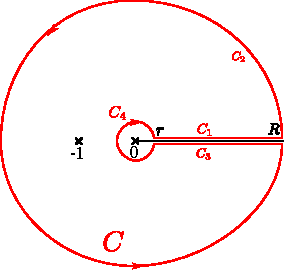
\includegraphics[width=7cm]{betaz1-z.pdf}
  \caption{カットを実軸正の部分に入れる。$C_1,\ C_3$はそれぞれ$r$から$R$までの間を実軸のすぐ上とすぐ下を通る経路。$C_2$は半径$R$の円周、$C_4$は半径$r$の円周。すべてを合わせたものを$C$とする。向きは矢印で表している。}
  \label{fig:betaz1-z}
\end{figure}

まず、留数を用いて評価しましょう。$C$の内側にある特異点は$s=-1$のみですから
\begin{align}
  \int_{C}\dd{s}f(s)=2\pi i \Resi_{s=-1}f(s)=2\pi i e^{-\pi i z}\label{gammaresidueintegral}
\end{align}
となります。留数は、今考えているブランチを慎重に考えて計算してください。

一方で$C=C_1+C_2+C_3+C_4$ですので、一つ一つ評価していきます。ここでは$0<\Re z <1$の場合を考えます。この場合に相補公式\eqref{reflectionformula}が証明できれば、いつものように一致の定理から両辺が定義されるすべての領域で成り立つことが証明できたことになります。さて、このとき
\begin{align}
  \lim_{r\to 0}\int_{C_4}\dd{s}f(s)=0,\quad
  \lim_{R\to \infty}\int_{C_2}\dd{s}f(s)=0
\end{align}
が成り立ちます。この式の証明は前にやったように不等式で丁寧に押さえていくことでできますが、ここでは省略します。$C_1,\ C_3$の部分に関しては、カットでの不連続性の積分になります。$t>0$として$f(t-i0)=e^{-2\pi i z}f(t+i0)$となるので
\begin{align}
  \int_{C_1}\dd{s}f(s)+\int_{C_3}\dd{s}f(s)
  =(1-e^{-2\pi i z})\int_{r}^{R}\dd{t}\frac{t^{-z}}{1+t}
  \to (1-e^{-2\pi i z})I\ (r\to 0,\ R\to \infty)
\end{align}
となります。式\eqref{gammaresidueintegral}と合わせると
\begin{align}
  I=\frac{2\pi i e^{-\pi i z}}{1-e^{-2\pi i z}}=\frac{2i\pi}{e^{\pi i z}-e^{-\pi i z}}=\frac{\pi}{\sin\pi z}
\end{align}
なので$B(1-z,z)=\frac{\pi}{\sin\pi z}$となり、式\eqref{tempreflection0}と合わせて公式\eqref{reflectionformula}が証明できました。

\subsection{応用}
まず、相補公式\eqref{reflectionformula}と無限積表示\eqref{gammainfiniteproduct}から、三角関数$\sin$の無限積表示を得ることができます。\eqref{reflectionformula}から
\begin{align}
  \frac{\sin \pi z}{\pi}
  &=\frac{1}{\Gamma(z)\Gamma(1-z)}
  =\frac{1}{(-z)\Gamma(z)\Gamma(-z)}\nonumber\\
  &=-\frac{1}{z}e^{\gamma z}z \prod_{k=1}^{\infty}\qty(1+\frac{z}{k})e^{-z/k}e^{-\gamma z}(-z)\prod_{k=1}^{\infty}\qty(1-\frac{z}{k})e^{z/k}
  =z\prod_{k=1}\qty(1-\frac{z^2}{k^2})
\end{align}
となります。ここで$\pi z=x$とおくと
\begin{important}
  \begin{align}
    \sin x = x \prod_{k=1}^{\infty}\qty(1-\frac{x^2}{\pi^2 k^2})
    \label{sininfiniteproduct}
  \end{align}
\end{important}
を得ます。

ここでは$\sin$の無限積表示\eqref{sininfiniteproduct}は、ちゃんとした導出をやりました。しかし、次のような形で予想することもできます。$\sin x$は多項式ではありませんが、多項式のような気分になって因数分解することを考えましょう。$\sin x=0$の方程式の解が$x=\pi k,\ k\in \Zb$
ですから$A$を定数として
\begin{align}
  \sin x = A x \prod_{k=1}^{\infty}\qty(1-\frac{x}{\pi k})\qty(1+\frac{x}{\pi k})
\end{align}
と因数分解できることが予想できます。$\lim_{x\to 0}\frac{\sin x}{x}=1$であることを用いると$A=1$となります。こうして\eqref{sininfiniteproduct}が予想できます。

\section{まとめ}
この章では、特殊関数の中でも物理で最も頻繁に現れるガンマ関数について勉強しました。やったことをまとめます。
\begin{itemize}
  \item ガンマ関数は定義\ref{:gammafunction}で定義されます。解析接続により$\Cb\setminus \{0,-1,-2,\dots\}$で正則関数になります。$0,-1,-2,\cdots$は1位の極です。
  \item 最も重要な公式は$\Gamma(z+1)=z\Gamma(z)$です。これから、ガンマ関数は階乗を正の整数以外に一般化したものであるということができます。
  \item 積分を近似する方法として鞍点法というものがあり、物理で頻繁に現れます。ガンマ関数に適用するとスターリングの公式が得られます。
  \item ガンマ関数に関して、様々な公式があります。
  \item ガンマ関数と関係が深いベータ関数という関数があります。
\end{itemize}


\chapter{直交多項式}

\section{関数の内積と直交関数系}
みなさんは、量子力学で関数同士の内積を考えることに慣れていると思います。ここでは、量子力学で勉強した関数同士の内積を少しだけ一般化したものを考えます。

まず、実数上の区間$(a,b),\ (a<b)$を考えます。$a=-\infty$でもよいですし、$b=+\infty$でもよいです。この区間での関数を考えます。

次に区間$(a,b)$上の関数$\rho(x)> 0$を1つとって固定します。この$\rho(x)$を\strong{重み関数}と呼びます。そして関数$f(x)$と$g(x)$の内積を
\begin{align}
  (f,g):=\int_{a}^{b} \dd{x} \rho(x) f(x)^{*} g(x) \label{innerproduct}
\end{align}
で定義します。これは、前の引数について反線形、後の引数について線形で$(f,f)\ge 0$、そして$(f,f)=0\ \Leftrightarrow \ f=0$\footnote{$f=0$の意味は、すべての$x$に対して$f(x)=0$という意味ではなく、$f(x)\ne 0$となる$x$の集合が測度$0$だということです。同じように$f=g$は、上の意味で$f-g=0$という意味です。}という正定値エルミート内積の公理を満たします。 \footnote{量子力学とのアナロジーのためにエルミート内積にしましたが、今後実関数のみを考えるので実対称内積と思っても良いです。}

この章でやりたいのは、内積での(正規)直交基底を考えることです。このような問題は量子力学を考える際に有用であることは、想像に難くないでしょう。

例えば次のようなものを考えてみましょう。
\begin{align}
  a=0,\ b=\pi,\ \rho(x)=1.
\end{align}
これは、量子力学でみなさん馴染みあると思います。この場合
\begin{align}
  f_{n}(x)=\sin nx\quad (n=1,2,3,\dots)
\end{align}
はある$k_n>0$で$(f_n,f_m)=k_n\delta_{m,n}$を満たす直交基底になります。

\section{直交多項式の導入}
この章で特に考えたいことは
\begin{myquote}
  直交基底として多項式をとってくることができるか?
\end{myquote}
という問題です。

グラム・シュミットの直交化を思い出すと、この問題の答えは肯定的な気がします。つまり次のように考えます。まず、
\begin{align}
  f_0(x):=1
\end{align}
とします。次に$g_1(x):=x$として
\begin{align}
  f_1(x):=g_1(x)-f_0(x)\frac{(f_0,g_1)}{(f_0,f_0)}
\end{align}
と定義します。右辺第2項目は$0$次式ですから、$f_1$は1次式です。また$(f_0,f_1)=0$であることが、次のようにして分かります。
\begin{align}
  (f_0,f_1)=(f_0,g_1)-(f_0,f_0)\frac{(f_0,g_1)}{(f_0,f_0)}=0.
\end{align}
さらに$g_2(x):=x^2$として
\begin{align}
  f_2(x):=g_2(x)-f_1(x)\frac{(f_1,g_2)}{(f_1,f_1)}-f_0(x)\frac{(f_0,g_2)}{(f_0,f_0)}
\end{align}
と定義します。右辺第2項目、第3項目は$g_2$の$f_0,f_1$のなす空間への射影ですから1次式です。なので$f_2$は2次式になります。また$(f_0,f_2)=(f_1,f_2)=0$が示せます。これを繰り返していきます。$f_0,\dots,f_{n-1}$が求まったとすると$g_{n}=x^{n}$として
\begin{align}
  f_{n}(x)=g_{n}(x)-\sum_{k=0}^{n-1}f_k(x)\frac{(f_k,g_n)}{(f_k,f_k)}
  \label{monicGram–Schmidt}
\end{align}
と定義します。このようにして$f_n\ (n=0,1,2,\dots)$が定義できます。

このようにして作った$f_n$は次の性質を満たします。
\begin{itemize}
  \item $f_n(x)$は$x$の$n$次多項式です。
  \item ある$k_n>0$があって$(f_n,f_m)=k_n\delta_{n,m}$という直交関係を満たします。
\end{itemize}
逆に、この2つを満たすような多項式の列$F_n\ (n=0,1,2,\cdots)$は、作り方から定数倍を除いて$f_n$と一致することが分かります。このような多項式の列を\strong{直交多項式}と呼びます。

直交多項式の規格化について少しコメントします。例えば次のような規格化はよく現れます。
\begin{itemize}
  \item $(f_n,f_n)=1$となる、つまり正規直交関係を満たすように規格化されたものを正規直交多項式と呼びます。
  \item $f_n(x)$の$x^n$の係数が$1$のように規格化されたものをモニック直交多項式と呼びます。
\end{itemize}
この節の最初にグラム・シュミットの直交化で作ったものはモニック直交多項式です。この2つの規格化以外のものもよく使われます。

これまでの一般論から分かる直交多項式の性質を少しずつ見ていきましょう。
まず、式\eqref{monicGram–Schmidt}より
\begin{align}
  x^n=(f_0,\dots,f_n \text{ の線形結合})
\end{align}
となります。したがって$h_k(x)$を任意の$k$次多項式とすると、これは$1,x,\dots,x^k$の線形結合ですから
\begin{align}
  h_k(x)=(f_0,\dots,f_k \text{ の線形結合})
\end{align}
となります。したがって$k<n$とすると
\begin{align}
  (f_n,h_k)=0\label{vanishinginnerproduct}
\end{align}
ということが言えます。

これをさらに推し進めていくと、一般に直交多項式は3項間漸化式を
\begin{align}
  xf_n(x)=\alpha_n f_{n+1}(x)+\beta_n f_n(x)+\gamma_n f_{n-1}(x)
  \label{recursionrelation3}
\end{align}
満たすことが分かります。ここで$\alpha_n,\beta_n,\gamma_n$は、ある定数です。
これを証明しましょう。$xf_n(x)$は$(n+1)$次多項式ですから$f_0,\dots,f_{n+1}$の線形結合で書けます。つまり、ある定数$c_{k}\ (k=0,1,\dots,n+1)$があって
\begin{align}
  xf_n(x)=\sum_{k=0}^{n+1}c_{k}f_{k}(x)
\end{align}
と表せるということです。直交性を用いることにより
\begin{align}
  c_k=\frac{(f_k,xf_n)}{(f_k,f_k)}
\end{align}
という式を得ます。内積の定義\eqref{innerproduct}より$(f_k,xf_n)=(xf_k,f_n)$となります。
$k<n-1$の場合を考えると、$xf_k$は$k+1$次多項式で$k+1<n$であることに注意して式\eqref{vanishinginnerproduct}を用いると$(xf_k,f_n)=0$となり、$c_k=0\ (k=0,\dots, n-2)$ということが示され、式\eqref{recursionrelation3}が示されました。

3項間漸化式は、$\alpha_n,\beta_n,\gamma_n$を何らかの方法で知ることができれば、直交多項式を計算する、実用的な方法になります。例えばモニック直交多項式の規格化をとれば、両辺の$x^{n+1}$の係数を比較することにより、$\alpha_n=1$となります。さらに、$a=-b,\ \rho(-x)=\rho(x)$であれば、$xf_n(x)$と$f_n(x)$は偶関数と奇関数が反対になるので$\beta_n=0$となります。この場合でも$\gamma_n$は別の何らかの方法で求める必要があります。

\section{ロドリゲスの公式}
\subsection{ロドリゲスの公式の導出}
最も一般的な直交多項式の議論は、これくらいにして、少し特殊な場合を考えましょう。具体的には区間$(a,b)$と重み関数$\rho(x)$が次の条件を満たす場合を考えます。
\begin{myquote}
ある$A(x),\ B(x)$があって次の3つの条件を満たす。
\begin{align}
 & \frac{\rho'(x)}{\rho(x)}=\frac{A(x)}{B(x)},\label{rhoprhoAB}\\
 & A(x)=a_0+a_1 x,\quad B(x)=b_0+b_1x + b_2 x^2\quad (a_0,a_1,b_0,b_1,b_2\text{:定数}),\label{ABdegree}\\
 & \lim_{x\to a}B(x)\rho(x)=\lim_{x\to b}B(x)\rho(x)=0.\label{surface}
\end{align}
\end{myquote}
この条件をロドリゲス条件と呼んでおきましょう\footnote{ロドリゲス条件という呼び方は一般的に使われるものではないと思います。ここだけの呼び方です。\eqref{rhoprhoAB}は\eqref{ABdegree}のもとでPearsonの微分方程式と呼ばれます。}。今後は、ロドリゲス条件を満たす区間と重み関数のみを考えます。

次の定理が成り立ちます。
\begin{theor}{ロドリゲスの公式}{thRodrigues}
$(a,b),\ \rho(x)$がロドリゲス条件を満たすとき、
\begin{align}
  F_n(x):=\rho(x)^{-1}\qty(\dv{x})^n\qty(\rho(x)B(x)^n)\quad (n=0,1,2,\dots)\label{Rodrigues}
\end{align}  
が$n$次多項式で直交多項式になる。
\end{theor}
式\eqref{Rodrigues}は(一般化された)ロドリゲスの公式と呼ばれます。

さて、ロドリゲスの公式を証明しましょう\footnote{この証明が載っている教科書は少ないです。ここの議論は、高橋 陽一郎(著)「実関数とフーリエ解析」(岩波書店)を参考にしました。}。証明のために、微分演算子
\begin{align}
  Q=\rho(x)^{-1}\dv{x} \rho(x)\label{RodriguesQ}
\end{align}
を定義し、次の補題を立てます。
\begin{lemma}{}{lemRodrigues}
  $g(x)$を任意の$\ell$次多項式とします。このとき$k\ge 1$として
  \begin{align}
    Q(g(x)B(x)^{k})=(\text{高々}(\ell+1)\text{次多項式})B(x)^{k-1}
  \end{align}
  と書けます。
\end{lemma}
この補題を証明をします。式\eqref{rhoprhoAB}を用いると
\begin{align}
  Q(g B^{k})=\rho^{-1}\dv{x}(\rho g B^k)
  =\rho^{-1}\rho' g B^k+ \rho^{-1}\rho g' B^k+\rho^{-1}\rho g kB^{k-1}B'
  =(Ag+g'B+kgB')B^{k-1}
\end{align}
となります。$A$は高々1次式、$g$は$\ell$次式、$B$は高々2次式であることを考慮すると、最後の式の$()$の中は、高々$(\ell+1)$次式であることが分かります。これで補題\ref{:lemRodrigues}が証明できました。

次に\eqref{Rodrigues}の$F_n(x)$が高々$n$次多項式であることを証明します。
まず、式\eqref{RodriguesQ}の$Q$を用いると、$F_n(x)=Q^n B^n$と書けます。補題\ref{:lemRodrigues}を用いて
\begin{align}
  F_n(x)=Q^nB^n=Q^{n-1}\qty[(\text{高々1次多項式})B^{n-1}]
  =\dots=(\text{高々$n$次多項式})B^{0}
\end{align}
というふうに示せます。

最後に直交性を示します。$m\ne n$のとき$(F_m,F_n)=0$を示すわけですが、$m>n$としても一般性を失いません。このとき
\begin{align}
  (F_m,F_n)
  &=\int_{a}^{b}\dd{x}\rho(x)F_m(x)F_n(x)
  =\int_{a}^{b}\dd{x}\dv[m]{x}(\rho(x)B(x)^m) F_n(x)\nonumber\\
  &=-\int_{a}^{b}\dd{x}\dv[m-1]{x}(\rho(x)B(x)^m) \dv{x}F_n(x)
  =\dots=(-1)^m\int_{a}^{b}\dd{x}\rho(x)B(x)^m \dv[m]{x}F_n(x)
\end{align}
となります。一行目から二行目に行くときには部分積分をし、\eqref{surface}の条件から表面項が消えることを用いました。二行目ではこれを繰り返しました。最後$F_n(x)$は高々$n$次式でこれを$m$回($m>n$)微分しているので$0$になります。これで直交性$(F_m,F_n)=0\ (m\ne n)$が示せました。直交多項式は定数倍を除いて一意でしたから、\eqref{Rodrigues}の$F_n\ (n=0,1,2,3)$が直交多項式であること、つまり定理\ref{:thRodrigues}が証明されました。

\subsection{直交多項式の例}\label{sec:exampleorthogonal}
ここまでは、かなり一般論をやってきましたが、ここでよく現れる直交多項式の例を3つ紹介します。

\paragraph{ルジャンドル多項式}
区間は$(-1,1)$で、重み関数は$\rho(x)=1$です。このとき
\begin{align}
  \frac{\rho'(x)}{\rho(x)}=0
\end{align}
ですので
\begin{align}
  A(x)=0,\quad B(x)=x^2-1
\end{align}
ととると条件\eqref{rhoprhoAB}、\eqref{ABdegree}、\eqref{surface}を満たすことができます。このときの直交多項式はロドリゲスの公式を用いて
\begin{important}
  \begin{align}
    P_{n}(x)=\frac{1}{2^n n!}\qty(\dv{x})^n((x^2-1)^n)\label{Legendre}
  \end{align}
\end{important}
と書けます。ただし規格化の定数は、よく使われているものを用いました。この直交多項式は\strong{ルジャンドル多項式}と呼ばれます。ルジャンドル多項式は球対称ポテンシャル中の粒子の量子力学に現れる球面調和関数などに現れます。

\paragraph{ラゲール多項式}
区間は$(0,\infty)$で、重み関数は$\rho(x)=e^{-x}$です。このとき
\begin{align}
  \frac{\rho'(x)}{\rho(x)}=-1
\end{align}
ですので
\begin{align}
  A(x)=-x,\quad B(x)=x
\end{align}
ととると条件\eqref{rhoprhoAB}、\eqref{ABdegree}、\eqref{surface}を満たすことができます。このときの直交多項式はロドリゲスの公式を用いて
\begin{important}
  \begin{align}
    L_{n}(x)=e^{x}\qty(\dv{x})^n(e^{-x}x^n)\label{Laguerre}
  \end{align}
\end{important}
と書けます。ここでも規格化は、よく使われるものを用いました。この直交多項式は\strong{ラゲール多項式}
と呼ばれます。ラゲール多項式は水素原子の動径方向の波動関数などに現れます。

\paragraph{エルミート多項式}
区間は$(-\infty,\infty)$で、重み関数は$\rho(x)=e^{-x^2}$です。このとき
\begin{align}
  \frac{\rho'(x)}{\rho(x)}=-2x
\end{align}
ですので
\begin{align}
  A(x)=-2x,\quad B(x)=1
\end{align}
ととると条件\eqref{rhoprhoAB}、\eqref{ABdegree}、\eqref{surface}を満たすことができます。このときの直交多項式はロドリゲスの公式を用いて
\begin{important}
  \begin{align}
    H_{n}(x)=(-1)^n e^{x^2}\qty(\dv{x})^n(e^{-x^2})\label{Hermite}
  \end{align}
\end{important}
と書けます。ここでも規格化は、よく使われるものを用いました。この直交多項式は\strong{エルミート多項式}
と呼ばれます。エルミート多項式は調和振動子の波動関数などに現れます。

これら以外にも、有用な直交多項式は、たくさんあります。

\subsection{規格化}
実際に使うには、規格化の定数を計算しておく必要があります。ロドリゲスの公式を用いると比較的見通しよく計算することができます。

区間$(a,b)$と重み関数$\rho(x)$が条件\eqref{rhoprhoAB}、\eqref{ABdegree}、\eqref{surface}を満たすとします。このとき直交多項式は\eqref{Rodrigues}の形
\begin{align}
  F_n(x)=\rho(x)^{-1}\qty(\dv{x})^n\qty(\rho(x)B(x)^n)
\end{align}
と書けます。このとき$(F_n,F_n)$を計算しましょう。
\begin{align}
  (F_n,F_n)
  &=\int_{a}^{b}\dd{x}\rho(x)F_n(x)F_n(x)\nonumber\\
  &=\int_{a}^{b}\dd{x}\qty(\dv{x})^n\qty(\rho(x)B(x)^n) F_n(x)
  =(-1)^n\int_{a}^{b}\dd{x}\qty(\rho(x)B(x)^n) \qty(\dv{x})^n F_n(x)
\end{align}
となります。ここでは、部分積分を何回も行い、条件\eqref{surface}から表面項が消えることを用いました。$F_n(x)$は$n$次多項式でしたから$\qty(\dv{x})^n F_n(x)$は定数になります。後は$\int_{a}^{b}\dd{x}\qty(\rho(x)B(x)^n)$の積分を、がんばって評価します。

例として、ルジャンドル多項式\eqref{Legendre}の場合に具体的に計算してみましょう。上と同じ変形をすると
\begin{align}
  (P_n,P_n)=(-1)^n\frac{1}{2^{2n} (n!)^2}\int_{-1}^{1}\dd{x}(x^2-1)^n\qty(\dv{x})^{2n}((x^2-1)^n)\label{templegendre1}
\end{align}
となります。まずは定数$\qty(\dv{x})^{2n}((x^2-1)^n)$を評価しましょう。$2n$回微分されているので$x^{2n}$より小さいべきはすべて消えることに注意すると
\begin{align}
  \qty(\dv{x})^{2n}((x^2-1)^n)=\qty(\dv{x})^{2n}(x^{2n})=(2n)!\label{templegendre2}
\end{align}
を得ます。次に積分$\int_{-1}^{1}\dd{x}(x^2-1)^n$を評価しましょう。$z=\frac{1-x}{2}$という変数変換をすると
\begin{align}
  \int_{-1}^{1}\dd{x}(x^2-1)^n
  &=\int_{1}^{0}(-2\dd{z})(-2z)^n(2(1-z))^n
  =(-1)^n2^{2n+1} \int_{0}^{1}\dd{z}z^n(1-z)^n\nonumber\\
  &=(-1)^n2^{2n+1} B(n+1,n+1)
  =(-1)^n2^{2n+1} \frac{\Gamma(n+1)\Gamma(n+1)}{\Gamma(2n+2)}\nonumber\\
  &=(-1)^n2^{2n+1} \frac{(n!)^2}{(2n+1)!}\label{templegendre3}
\end{align}
となります。ここではベータ関数の定義\eqref{betaintegral}とガンマ関数との関係\eqref{betagamma}、そしてガンマ関数の値\eqref{gammafactorial}を用いました。式\eqref{templegendre2}と式\eqref{templegendre3}を式\eqref{templegendre1}に代入すると
\begin{align}
  (P_n,P_n)=\frac{2}{2n+1}
\end{align}
を得ます。

他の直交多項式の場合も同様の方針で計算することが可能です。例えばラゲール多項式\eqref{Laguerre}の場合
\begin{align}
  (L_n,L_n)=(n!)^2
\end{align}
となります。またエルミート多項式\eqref{Hermite}の場合には
\begin{align}
  (H_n,H_n)=2^n n!\sqrt{\pi}
\end{align}
となります。ぜひチェックしてみてください。

\section{直交多項式の満たす微分方程式}
ロドリゲス条件を満たすような直交多項式の面白いところは、ロドリゲスの公式が成り立つということだけでなく、ある2階の微分方程式を満たすところです。このために物理に頻繁に現れます。ここでは、直交多項式の満たす微分方程式について説明します。

次の定理が成り立ちます。
\begin{theor}{}{orthogonaldiffeq}
  条件\eqref{rhoprhoAB}、\eqref{ABdegree}、\eqref{surface}を満たすような区間$(a,b)$と重み関数$\rho(x)$に対する直交多項式\eqref{Rodrigues}は、微分方程式
  \begin{align}
    B(x)F_n''(x)+(A(x)+B'(x))F_n'(x)-\alpha_n F_n(x)=0\label{orthogonaldiffeq}
  \end{align}
  を満たす。ここで
  \begin{align}
    \alpha_n=n(n+1)b_2+na_1
  \end{align}
  である。$b_2,a_1$は\eqref{ABdegree}で定義されている。
\end{theor}
これは、後で出てくる超幾何微分方程式、あるいは合流型超幾何微分方程式になります。言い換えると直交多項式は、超幾何関数、あるいは合流型超幾何関数であって、かつ多項式になるものです。多項式になるというのは、量子力学での波動関数の規格化可能性と関係して、頻繁に現れる理由になっています。

証明は後回しにして、\ref{sec:exampleorthogonal}でやった例がどんな微分方程式を満たすかを見ておきましょう。

まず、ルジャンドル多項式では
\begin{align}
  (a,b)=(-1,1),\quad \rho(x)=1,\quad A(x)=0,\quad B(x)=x^2-1
\end{align}
でしたから、定理\ref{:orthogonaldiffeq}に当てはめると
\begin{align}
  (x^2-1)P_n''(x)+2x P_n'(x)-n(n+1)P_n(x)=0
\end{align}
という微分方程式を満たします。この方程式は球対称ポテンシャル中のシュレーディンガー方程式を変数分離したもののうち$\theta$方向に現れます。

次に、ラゲール多項式では
\begin{align}
  (a,b)=(0,\infty),\quad \rho(x)=e^{-x},\quad A(x)=-x,\quad B(x)=x
\end{align}
でしたから、定理\ref{:orthogonaldiffeq}に当てはめると
\begin{align}
  xL_n''(x)+(1-x) L_n'(x)+nL_n(x)=0
\end{align}
という微分方程式を満たします。これは水素原子のシュレーディンガー方程式を変数分離したもののうちS軌道の場合の動径方向に現れます。

最後に、エルミート多項式では
\begin{align}
  (a,b)=(-\infty,\infty),\quad \rho(x)=e^{-x^2},\quad A(x)=-2x,\quad B(x)=1
\end{align}
でしたから、定理\ref{:orthogonaldiffeq}に当てはめると
\begin{align}
  H_n''(x)-2x H_n'(x)+2n H_n(x)=0
\end{align}
という微分方程式を満たします。これは調和振動子のシュレーディンガー方程式に現れます。

\subsection{定理の証明}
さて定理\ref{:orthogonaldiffeq}を証明しましょう。まず、\eqref{orthogonaldiffeq}の左辺第1項、第2項は高々$n$次多項式ですから$F_0(x),\dots,F_n(x)$の線形結合で表すことができます。
\begin{align}
  B(x)F_n''(x)+(A(x)+B'(x))F_n'(x)=\sum_{k=0}^{n}C_k F_k(x).\label{temporthdiff}
\end{align}
ですから、次の2つのことを示せれば定理\ref{:orthogonaldiffeq}が証明されます。
\begin{itemize}
  \item[① ] $C_n=\alpha_n$
  \item[② ] $C_k=0\ (k=0,1,2,\dots,n-1)$ 
\end{itemize}

まず①からいきましょう。これは式\eqref{temporthdiff}の両辺で$x^n$の係数を比較することで得られます。
$F_n(x)$の規格化は、よく分からないので、ひとまず
\begin{align}
  F_n(x)=h_n x^n +((n-1)\text{次以下}),\quad h_n\ne 0
\end{align}
としておきます。すると\eqref{temporthdiff}の左辺は
\begin{align}
  (\text{左辺})=b_2 n(n-1)h_n x^n+(a_1+2b_2)n h_n x^n+((n-1)\text{次以下})=\alpha_n h_n x^n+((n-1)\text{次以下})
\end{align}
となります。一方\eqref{temporthdiff}の右辺は
\begin{align}
  (\text{右辺})=C_nh_nx^n+((n-1)\text{次以下})
\end{align}
となります。両辺を比較すると$h_n$は両辺から割ることができて
\begin{align}
  C_n=\alpha_n
\end{align}
を得ます。これで①を示せました。

一方で②は、\eqref{temporthdiff}の左辺を
\begin{align}
  g(x):=B(x)F_n''(x)+(A(x)+B'(x))F_n'(x)
\end{align}
と書いたとき、$(g,F_k)=0 \ (k<n)$を示せば良いことになります。ところで
\begin{align}
  g(x)=\frac{1}{\rho}\dv{x}\qty(\rho B F_n')
\end{align}
であることが、実際に右辺の微分を実行し、\eqref{rhoprhoAB}を用いることで分かります。これを用いると
\begin{align}
  (g,F_k)
  &=\int_{a}^{b}\dd{x}\rho(x) g(x)F_k(x)
  =\int_{a}^{b}\dd{x} \dv{x}\qty(\rho B F_n')F_k(x)\nonumber\\
  &=-\int_{a}^{b}\dd{x} \rho B F_n'F_k'(x)
  =\int_{a}^{b}\dd{x} F_n \dv{x}\qty(\rho B F_k'(x))
  =(F_n,q)\label{temporthdiff2}
\end{align}
となります。ここで$q(x):=\rho^{-1}\dv{x}\qty(\rho B F_k'(x))$と定義しました。これは、\eqref{RodriguesQ}の演算子を用いると$q=Q(F'_k B)$と書けます。したがって、補題\ref{:lemRodrigues}を用いると$q(x)$は高々$k$次式であることが分かります。
% この関数を\eqref{rhoprhoAB}などを用いて、よく調べてみると
% \begin{align}
%   q(x)
%   =\rho^{-1}\dv{x}\qty(\rho B F_k'(x))
%   =\rho^{-1}\qty(\rho' B F_k'(x)+\rho B' F_k'(x)+\rho B F_k''(x))
%   =A F_k'(x)+ B' F_k'(x)+ B F_k''(x)
% \end{align}
% となります。\eqref{ABdegree}を考慮すると$q(x)$は高々$k$次式であることが分かります。
$k<n$ですから式\eqref{temporthdiff}より$(g,F_k)=(F_n,q)=0$となり、②が示せました。

これで定理\ref{:orthogonaldiffeq}が証明できました。

\section{直交多項式の母関数}
ここでは、直交多項式の母関数について考えてみましょう。直交多項式を$f_n(x)\ (n=0,1,2,\dots)$として
\begin{align}
  G(x,t):=\sum_{n=0}^{\infty}\frac{t^n}{n!}f_n(x)
\end{align}
のような関数を\strong{母関数}と呼びます。$t$についてテイラー展開したときの各係数に直交多項式が現れるような関数ですね。直交多項式は難しくても、母関数は簡単な形をしていることが多いです。あと係数の規格化は、場合に応じて便利なものが選ばれていることに注意してください。

これまで出てきた直交多項式の例では、母関数は次のようになっています。
\begin{important}
\begin{itemize}
  \item ルジャンドル多項式の母関数
  \begin{align}
    \sum_{n=0}^{\infty}P_n(x)t^n=\frac{1}{\sqrt{1-2xt+t^2}}.\label{Legendregenfunc}
  \end{align}  
  \item ラゲール多項式の母関数
  \begin{align}
    \sum_{n=0}^{\infty}L_n(x)\frac{t^n}{n!}=\frac{e^{\frac{tx}{t-1}}}{1-t}.
  \end{align}  
  \item エルミート多項式の母関数
  \begin{align}
    \sum_{n=0}^{\infty}H_n(x)\frac{t^n}{n!}=e^{2xt-t^2}.
  \end{align}
\end{itemize}
\end{important}

直交多項式の母関数の求め方について説明します。
区間$(a,b)$と重み関数$\rho(x)$が、ロドリゲス条件\eqref{rhoprhoAB},\eqref{ABdegree},\eqref{surface}を満たす場合を考えることにしましょう。この場合には対応する直交多項式の母関数は次のような手順で求めることができます。

まず、用いるのはコーシーの積分公式です。$x$を含む領域$D$で正則な関数$f$に対して
\begin{align}
  f(x)=\frac{1}{2\pi i}\oint_{C_x}\dd{\xi} \frac{f(\xi)}{\xi-x}
  \label{Cauchyintegralformula}
\end{align}
が成り立ちます。ただし、$C_x$は$x$を反時計回りに囲む経路で$C_x$自身と内部も$D$に含まれるようなものとします。式の両辺を$n$階微分すると
\begin{align}
  f^{(n)}(x)=\frac{n!}{2\pi i}\oint_{C_x}\dd{\xi} \frac{f(\xi)}{(\xi-x)^{n+1}}\label{Goursatintegralformula}
\end{align}
という式を得ます。この式はグルサ(Goursat)の積分公式とも呼ばれます。

直交多項式
\begin{align}
  F_n(x)=
  \frac{1}{\rho(x)}\qty(\dv{x})^n(\rho(x)B(x)^n)
\end{align}
をグルサの積分公式\eqref{Goursatintegralformula}を用いて変形します。すると
\begin{align}
  F_n(x)=\frac{1}{\rho(x)}\frac{n!}{2\pi i}\oint_{C_x}\dd{\xi} \frac{\rho(\xi)B(\xi)^n}{(\xi-x)^{n+1}}
\end{align}
を得ます。これを用いて母関数を計算していきます。
\begin{align}
  G(x,t)&:=\sum_{n=0}^{\infty}F_n(x)\frac{t^n}{n!}
  =\frac{1}{2\pi i \rho(x)}\oint_{C_x}\dd{\xi}\sum_{n=0}^{\infty}\frac{\rho(\xi)B(\xi)^n}{(\xi-x)^{n+1}}t^n\nonumber\\
  &=\frac{1}{2\pi i \rho(x)}\oint_{C_x}\dd{\xi}\frac{\rho(\xi)}{\xi-x}\frac{1}{1-\frac{tB(\xi)}{\xi-x}}\nonumber\\
  &=\frac{1}{2\pi i \rho(x)}\oint_{C_x}\dd{\xi}\frac{\rho(\xi)}{\xi-x-tB(\xi)}\label{tempgeneratingfunction}
\end{align}
を得ます。ただしこの式変形が正しいためには一様絶対収束する条件
\begin{align}
  \qty|\frac{tB(\xi)}{\xi-x}|<1\label{tempconvergentcondition}
\end{align}
を満たしていなければならないことに注意してください。これを満たすように経路$C_x$をとる必要があります。式\eqref{tempgeneratingfunction}まで来たら、後はこの積分を留数を用いて評価してやれば良いです。特異点は分母が$0$になるところです。分母は高々2次式ですから特異点は多くても2個です。\eqref{tempconvergentcondition}に注意しながら、どの特異点が$C_x$の内側にあるかを調べ、そこでの留数を求めれば良いです。

具体例としてルジャンドル多項式の場合をやってみましょう。このとき
\begin{align}
  \rho(x)=1,\quad B(x)=x^2-1
\end{align}
です。ですから、式\eqref{tempgeneratingfunction}の被積分関数の特異点、つまり(分母)$=0$の解は
\begin{align}
  \xi=\xi_{\pm}:=\frac{1}{2t}(1\pm\sqrt{1-4t(x-t)})\label{xipole}
\end{align}
となります。また、条件\eqref{tempconvergentcondition}を満たすために非常に小さな$t$を考えることにしましょう。すると\eqref{xipole}の2つの特異点は$\xi_{-}$は非常に$x$に近く、$\xi_{+}$は非常に大きくなります。さらに条件\eqref{tempconvergentcondition}を詳しく調べると、$C_x$は図\ref{fig:genfunc}のように$\xi_{-}$を含むようにとり、$\xi_{+}$は含まないようにとらなければならないことが分かります。これを理解するためには、例えば次のように具体的に考えれば良いです。$x$は$0<x<1$の実数とし、$t$は$t>0$で十分小さいとします。すると$0<\xi_{-}<x<\xi_{+}$となります。この条件で$\frac{tB(\xi)}{\xi-x}$のグラフを描いてみたのが図\ref{fig:genfunc2}です。$\xi=\xi_{\pm}$のみで$1$を切ること、$\xi=x$が極であること、そして$\xi\to \pm \infty$でそれぞれ$\pm \infty$に行くことに注意してください。これを見ると$\xi>x$で$C_x$が実軸を切る点は$\xi_{+}$より小さくなくてはならず、$\xi<x$で$C_x$が実軸を切る点は$\xi_{-}$より小さくなければなりません。なので$C_{x}$は$\xi_{-}$を内部に含んで$\xi_{+}$を含まない図\ref{fig:genfunc}のような形になることが分かります。
\begin{figure}[htbp]
  \centering
  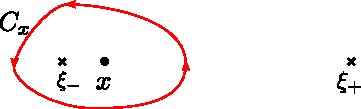
\includegraphics{genfunc.pdf}
  \caption{}
  \label{fig:genfunc}
\end{figure}
\begin{figure}[htbp]
  \centering
  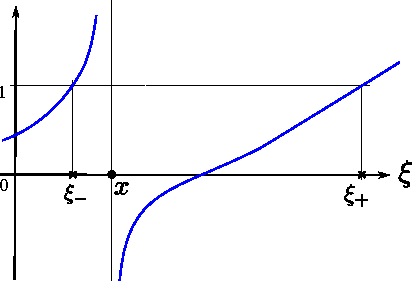
\includegraphics{genfunc2.pdf}
  \caption{}
  \label{fig:genfunc2}
\end{figure}

したがって、\eqref{tempgeneratingfunction}は、$\xi=\xi_{-}$の留数で評価できて
\begin{align}
  \sum_{n=0}^{\infty}F_n(x)\frac{t^n}{n!}
  =\Resi_{\xi=\xi_{-}}\frac{1}{-t(\xi-\xi_{-})(\xi-\xi_{+})}
  =\frac{1}{-t(\xi_{-}-\xi_{+})}
  =\frac{1}{\sqrt{1-4tx+4t^2}}
\end{align}
となります。ところで、ルジャンドル多項式のよく使われる規格化は$P_n(x)=\frac{1}{2^n n!}F_{n}(x)$でしたから、これを上の式に代入して
\begin{align}
  \sum_{n=0}^{\infty}P_n(x)(2t)^n=\frac{1}{\sqrt{1-4tx+4t^2}}
\end{align}
を得ます。両辺は$t$についての恒等式ですから$2t$のことを改めて$t$と書くと
\begin{align}
  \sum_{n=0}^{\infty}P_n(x)t^n=\frac{1}{\sqrt{1-2tx+t^2}}  
\end{align}
という\eqref{Legendregenfunc}の表式が得られます。

一つ応用例を紹介します。これは電磁気などで双極子モーメント、あるいはさらに多重極展開をするときに出てくる式です。$\rb$と$\rb'$を2つの3次元ベクトルとします。$|\rb|=:r,\ |\rb'|=:r'$として、$r'\ll r$の場合
\begin{align}
  \frac{1}{|\rb-\rb'|}\cong \frac{1}{r}+\frac{\rb\cdot\rb'}{r^3}
\end{align}
のような式が電磁気で双極子モーメントをやるときに出てきたと思います。この展開のさらに先はどうなるでしょうか。$\rb$と$\rb'$のなす角を$\theta$として
\begin{align}
  \frac{1}{|\rb-\rb'|}
  =\frac{1}{\sqrt{|\rb-\rb'|^2}}
  =\frac{1}{\sqrt{r^2-2rr'\cos\theta+r'^2}}
  =\frac{1}{r}\frac{1}{\sqrt{1-2\cos\theta\frac{r'}{r}+\qty(\frac{r'}{r})^2}}
\end{align}
と書くことができます。ここで$t=\frac{r'}{r},\ x=\cos\theta$として\eqref{Legendregenfunc}を用いると
\begin{align}
  \frac{1}{|\rb-\rb'|}=\frac{1}{r}\sum_{n=0}^{\infty}
  P_n(\cos\theta)\qty(\frac{r'}{r})^n
\end{align}
という展開式が得られます。ここから分かるように電磁気学で込み入ったことをやろうとすると、ルジャンドル多項式を活用する必要があります。


\section{まとめ}
この章では、直交多項式について学びました。やったことをまとめておきます。
\begin{itemize}
  \item ある区間と重み関数を与えたときの直交基底として多項式を考えると便利なことが多いです。このような多項式を直交多項式と呼びます。
  \item 直交多項式の中でもロドリゲス条件を満たすものに関しては、さらに深く調べることができます。特にロドリゲスの公式と呼ばれる表示が得られます。
  \item そのような直交多項式の例として、最も頻繁に現れるルジャンドル多項式、ラゲール多項式、エルミート多項式を紹介しました。
  \item ロドリゲス条件を満たす直交多項式は、ある2階の微分方程式を満たします。このため量子力学などに頻繁に現れます。
  \item 直交多項式の母関数を考えると便利なことが多いです。
\end{itemize}


\section{その他の直交多項式*}
この授業では直交多項式の例としてルジャンドル多項式、ラゲール多項式、エルミート多項式のみを取り扱いました。実は他にも物理でよく現れる直交多項式があります。この節では、それらの直交多項式についてまとめておきます。この節の内容は授業の中では説明しません。

\subsection{ヤコビ多項式とその仲間}
区間$(-1,1)$で重み関数が$\rho(x)=(1-x)^{\alpha}(1+x)^{\beta},\ (\alpha,\beta >-1)$の直交多項式はヤコビ(Jacobi)多項式と呼ばれます。$\alpha=\beta=0$の場合には、ルジャンドル多項式になります。なのでヤコビ多項式はルジャンドル多項式を一般化したものということが出来ます。ヤコビ多項式の区間と重み関数は、次のようにロドリゲス条件を満たします。
\begin{align}
  \frac{\rho'(x)}{\rho(x)}=\frac{A(x)}{B(x)},\quad A(x)=-\alpha-\beta+(-\alpha+\beta)x,\quad B(x)=x^2-1.
\end{align}
ですから、ヤコビ多項式はロドリゲスの公式で表すことが出来ます。よく使われる記号と規格化は
\begin{align}
  P^{\alpha,\beta}_n(x)=\frac{1}{2^n n!(1-x)^{\alpha}(1+x)^{\beta}}\qty(\dv{x})^n((1-x)^{\alpha}(1+x)^{\beta}(x^2-1)^n)
\end{align}
です。ヤコビ多項式の生成母関数は
\begin{align}
  \sum_{n=0}^{\infty}P_{n}^{(\alpha,\beta)}(x)t^n=
  \frac{2^{\alpha+\beta}}{\sqrt{1-2xt+t^2}(1+\sqrt{1-2xt+t^2}-z)(1+\sqrt{1-2xt+t^2}+z)}
\end{align}
と表せます。

ヤコビ多項式のうちよく現れる特殊な場合には名前がついています。例えば$\alpha=\beta=\lambda-\frac12$の場合には、ゲーゲンバウアー(Gegenbauer)多項式と呼ばれます。つまり、ゲーゲンバウアー多項式は、区間が$(-1,1)$で重み関数が$\rho(x)=(1-x^2)^{\lambda-\frac12}$の直交多項式です。よく使われる記号と規格化は
\begin{align}
  C^{(\lambda)}_{n}=\frac{(2\lambda)_n}{2^n (\lambda+\frac12)_n n!(1-x^2)^{\lambda-\frac12}}
  \qty(\dv{x})^n((1-x^2)^{\lambda-\frac12}(x^2-1)^n)
\end{align}
です。ここで$(a)_n$はポッホハマー記号と呼ばれる記号で、
\begin{align}
  (a)_n:=\frac{\Gamma(a+n)}{\Gamma(a)}=a(a+1)\dots(a+n-1)
\end{align}
で定義されています。ゲーゲンバウアー多項式の生成母関数は
\begin{align}
  \sum_{n=0}^{\infty}C^{(\lambda)}_{n}t^n=(1-2xt+t^2)^{-\lambda}
\end{align}
と表せます。

さらにゲーゲンバウアー多項式で$\lambda=0$としたものはチェビシェフ(Chebyshev)多項式と呼ばれます。つまりチェビシェフ多項式は区間$(-1,1)$で重み関数が$\rho(x)=(1-x^2)^{-\frac12}$の場合の直交多項式です

。よく使われる記号と規格化は
\begin{align}
  T_n(x)=\frac{1}{(2n-1)!!}(1-x^2)^{\frac12}
  \qty(\dv{x})^n((1-x^2)^{-\frac12}(x^2-1)^n)
\end{align}
です。ここで$!!$の記号は二重階乗と呼ばれるもので
\begin{align}
  (2n-1)!!:=1\cdot 3\cdot 5 \cdot \dots \cdot (2n-1)
  =2^n(\frac12)_n=\frac{(2n)!}{2^n n!}
\end{align}
を表します。チェビシェフ多項式の生成母関数は
\begin{align}
  \sum_{n=0}^{\infty}T_n(x)t^n = \frac{1-xt}{1-2xt+t^2}
\end{align}
と表せます。

\subsection{ソニン多項式とその仲間}
区間$(0,\infty)$で重み関数$\rho(x)=x^{\alpha}e^{-x},\ \alpha>-1$を考えます。このときの直交多項式を一般にソニン(Sonine)多項式と呼びます。これは、ラゲール多項式を一般化したものということができます。これは次のようにロドリゲス条件を満たします。
\begin{align}
  \frac{\rho'(x)}{\rho(x)}=\frac{A(x)}{B(x)},\quad A(x)=\alpha-x,\quad B(x)=x.
\end{align}
ですから、ソニン多項式はロドリゲスの公式で表すことができます。よく使われる記号と規格化は
\begin{align}
  S^{\alpha}_{n}(x)=\frac{1}{n!}x^{-\alpha}e^{x}\qty(\dv{x})^n(x^{\alpha+n}e^{-x})
\end{align}
です。生成母関数は
\begin{align}
  \sum_{n=0}^{\infty}S^{\alpha}_{n}(x)t^n=(1-t)^{-\alpha-1}e^{\frac{xt}{t-1}}
\end{align}
と表せます。

多くの量子力学の教科書水素原子のところに出てくるラゲール陪多項式は、ソニン多項式と関係があって、$m,n$が非負の整数で$n\ge m$を満たすとき
\begin{align}
  L^{m}_{n}(x)=(-1)^m n! S^{m}_{n-m}(x)
\end{align}
となります。ただし、このあたりの言葉遣いは文献によって異なっていて、例えば
\url{https://dlmf.nist.gov/}やWikipedia、岩波公式集などでは、
\begin{align}
  L_{n}^{(\alpha)}(x)=S^{\alpha}_{n}(x)
\end{align}
と書いて、これを単にラゲール多項式(Laguerre polynomials)、一般化されたラゲール多項式(generalized Laguerre polynomials)、ラゲール陪多項式(associated Laguerre polynomials)と呼んでいるので注意が必要です。

\chapter{微分方程式}\label{sec:ode}
\section{言葉など}
この章では、微分方程式について考えていきます。まず、ここで出てくる言葉を説明します。

$y$が$x$の未知の関数とします。1階微分、2階微分をそれぞれ$y',y''$と書きます。$n$階微分を$y^{(n)}$と書きます。ここで、$x,y,y',y'',\dots,y^{(n)}$を含む方程式
\begin{align}
  F(x,y,y',\dots,y^{(n)})=0
\end{align}
を\strong{($n$階)微分方程式}と呼びます。$F(...)$は与えられた関数です。このような微分方程式で$x$を\strong{独立変数}、$y$を\strong{従属変数}と呼びます。実数の枠内で考えることもありますし、複素数に広げて考えることもあります。

拡張の1つは、従属変数を増やすことです。$\yv=(y_1,y_2,\dots,y_N)$とし、それぞれの成分$y_i=y_i(x)\ (i=1,2,\dots,N)$が$x$の関数とします。このとき$N$個の方程式の組
\begin{align}
  F_i(x,\yv,\yv',\dots,\yv^{(n)})=0\quad (i=1,\dots,N)
\end{align}
も\strong{微分方程式}と呼びます。とくに従属変数がたくさんある場合は連立微分方程式と呼ばれることもあります。

では、独立変数を増やすとどうなるでしょうか。独立変数を$x_1,\dots,x_m$として、$y$をこれらの関数、つまり$y=y(x_1,\dots,x_m)$とします。このとき、使える微分は偏微分で
\begin{align}
  \pdv{y}{x_a},\ \pdv{y}{x_a}{x_b},\dots\qquad (a,b=1,\dots,m)
\end{align}
のようなものです。これらの偏微分を含んだ方程式を\strong{偏微分方程式}と呼びます。これに対して先程やった独立変数が1つの場合を\strong{常微分方程式}と呼びます。一般に偏微分方程式は常微分方程式より難しいです。偏微分方程式の最も基本的な解き方は常微分方程式に帰着させることです。この講義では、常微分方程式のみを取り扱います。

一般に高階の微分方程式は、従属変数を増やすことにより1階の連立微分方程式にすることができます。例えば、
\begin{align}
  F(x,y_1,y_1',y_1'')=0
\end{align}
という2階の微分方程式が与えられたとしましょう。このとき
$y_2:=y_1'$と定義することにより
\begin{align}
  F(x,y_1,y_2,y_2')=0,\quad y_2-y_1'=0
\end{align}
という、1階の連立微分方程式にすることができます。
このような操作は物理でも出てきます。ニュートンの運動方程式は、位置に対する2階の微分方程式です。それに対してハミルトンの正準運動方程式は、位置と運動量に対する1階の連立微分方程式になっています。このような操作は単純ですが、見通しをよくすることがあります。

\section{解の存在と一意性}\label{sec:exsistenceofsolution}
ここでは、微分方程式が「そんなに特異的ではない」場合には、初期条件を満たす解が存在して一意的であることを述べます。

従属変数が1つの、1階の微分方程式を考えます。特に、$y'$について解けて
\begin{align}
  y'=f(x,y)\label{ode1}
\end{align}
と書ける場合を考えます。さらに初期条件として
\begin{align}
  y(x_0)=y_0\label{initialcond}
\end{align}
を課します。このとき次の定理が成り立ちます。
\begin{theor}{解の存在と一意性}{exsistenceofsolution}
  $xy$平面内の$(x_0,y_0)$を含む領域$D$内で$f(x,y)$が次の①②③の条件を満たす場合、初期条件\eqref{initialcond}のもとで微分方程式\eqref{ode1}の解は$D$内にある限り一意的に存在する。
  \begin{itemize}
    \item[①] $f(x,y)$は連続
    \item[②] (「Lipschitz条件」)$\exists K\in \Rb$が存在して、$x$座標が同じ任意の2点$\forall (x,y_1),(x,y_2)\in D$ に対して
    \begin{align}
      |f(x,y_1)-f(x,y_2)|< K|y_1-y_2|
    \end{align}
    \item[③] $\exists M \in \Rb$が存在して
    \begin{align}
      |f(x,y)|<M,\quad \forall (x,y)\in D
    \end{align}
    を満たす。
  \end{itemize}
\end{theor}
証明は省略します。興味ある方は例えば寺沢寛一著「自然科学者のための数学概論」などを参照してください。

この定理に関して、少しコメントをします。
\begin{itemize}
  \item もし、$D$内で$\pdv{y}f(x,y)$が存在して有界なら②は満たされます。
  \item ②の感じをつかんでもらうために、②を満たさない例を挙げます。$f(x,y)=\sqrt{|y|}$は、$y=0$を含む領域で②を満たしません。②は$x$が一定の場合の弦の傾きが有界ということですが、この例では、$y=0$から引いた弦でいくらでも急なものがあります(図\ref{fig:singular}参照)。
  \item 1階連立微分方程式にも同様の定理があります。
  \item 高階の微分方程式に対しては、前節の最後に述べた方法で1階化すれば、この定理を適用できます。
\end{itemize}
\begin{figure}[htbp]
  \centering
  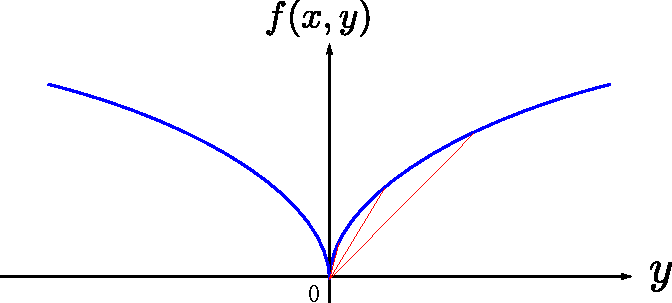
\includegraphics{singular.pdf}
  \caption{条件②を満たさない例。$y=0$の近くで、いくらでも傾きの大きい弦が存在する。}
  \label{fig:singular}
\end{figure}

我々が微分方程式を考えることの1つの目的は、新しい関数を微分方程式で定義したいということでした。このときには、この解の存在と一意性の定理は非常に重要な意味を持ちます。

\section{一般解と特異解}
ここで一般解と特異解という概念を導入したいと思います。

まず、定理\ref{:exsistenceofsolution}の①②③の条件を満たすような場合を考えてみましょう。そうすると例えば$x=x_0$の$y$の値によって解は一意的に指定されます。解のグラフは$D$全体を覆っていて交わったりしません。したがって、このような解は任意定数一つを含んでいます。このように定理\ref{:exsistenceofsolution}の①②③の条件を満たすような場合に任意定数1つを含む解を\strong{一般解}と呼びます。一般解が求まれば、後はなんらかの条件で任意定数を決定できれば、解が一つに定まります。

一階の連立微分方程式の場合にも同様の考察ができます。$x=x_0$のときの$\yv=(y_1,y_2,\dots,y_N)$の値によって解が決まりますから、任意定数$N$個を含む解が一般解になります。

さらに、独立変数が1つで$n$階微分方程式の場合には、$n$個の独立変数を用意することによって一階化できます。したがって、$n$個の任意定数を含む解が一般解です。

一方、定理\ref{:exsistenceofsolution}の①②③の条件を満たさない場合には、一般解ではない解が存在します。このような解を\strong{特異解}と呼びます。

特異解について例で説明しましょう。微分方程式
\begin{align}
  y'=\sqrt{|y|}\label{exsingular}
\end{align}
を考えましょう。これは\ref{sec:exsistenceofsolution}で見たように$y=0$で定理\ref{:exsistenceofsolution}の①②③の条件を満たさない例です。$y=0$以外の部分では、次のように初等的に解けます。
\begin{itemize}
  \item $y>0$のとき
  \begin{align}
    y'=\sqrt{y}
  \end{align}
  となりますから、変数分離で解けます。解は$C$を任意定数として
  \begin{align}
    y=\frac{1}{4}(x-C)^2
  \end{align}
  となります。ただし、\eqref{exsingular}を見ると$y'>0$ですから
  \begin{align}
    x>C
  \end{align}
  でなければなりません。
  \item $y<0$のとき
  \begin{align}
    y'=\sqrt{-y}
  \end{align}
  となりますから、やはり変数分離で解けます。解は$C$を任意定数として
  \begin{align}
    y=-\frac{1}{4}(x-C)^2
  \end{align}
  となります。同様に$y'>0$の条件を考えると
  \begin{align}
    x<C
  \end{align}
  でなければなりません。
\end{itemize}
さらに直接$y=0$を式\eqref{exsingular}に代入することにより、これが解であることが分かります。$y=0$は、一般解のどれとも異なることに注意してください。この$y=0$が今の例の特異解です。これらをプロットしたのが図\ref{fig:singularsolution}です。これを見ると特異解は、すべての一般解に接していることが分かります。このようなある曲線の集合のすべての元に接しているような曲線を\strong{包絡線}と呼びます。特異解は一般に一般解の包絡線になっています。
\begin{figure}[htbp]
  \centering
  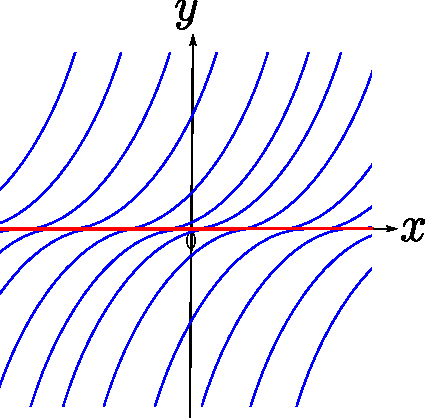
\includegraphics{singularsolution.pdf}
  \caption{$y'=\sqrt{|y|}$の様子。青が一般解。赤が特異解。}
  \label{fig:singularsolution}
\end{figure}


\section{線形微分方程式}
線形微分方程式は、微分方程式の中でも比較的系統的に調べることができる微分方程式です。ここで、線形微分方程式について事実をまとめておきます。

従属変数は1つとして、次のような形の微分方程式を$n$階\strong{斉次線形微分方程式}と呼びます。
\begin{align}
  y^{(n)}+a_{n-1}(x)y^{(n-1)}+\dots+a_1(x)y'+a_0(x)y=0.\label{homlinode}
\end{align}
ここで$a_i(x)\ (i=0,\dots,n-1)$は与えられた$x$の関数です。斉次線形微分方程式の著しい特徴は、$y_1,y_2$が\eqref{homlinode}の解である場合、$A,B$を定数として
\begin{align}
  y=Ay_1+By_2
\end{align}
も解であるということです。つまり、\eqref{homlinode}の解全体はベクトル空間をなしています。したがって、$n$個の独立な解$y_1,\dots,y_n$が求まったとすると、一般解は
\begin{align}
  y=C_1y_1+C_2y_2+\dots+C_ny_n\quad (C_1,\dots,C_n:\text{任意定数})
\end{align}
と書けます。つまり、斉次線形微分方程式を解くには、何らかの方法で独立な$n$個の解を求めれば良いです。

次に、式\eqref{homlinode}を少しだけ変えて
\begin{align}
  y^{(n)}+a_{n-1}(x)y^{(n-1)}+\dots+a_1(x)y'+a_0(x)y=b(x)
  \label{inhomlinode}
\end{align}
としたものを考えてみましょう。右辺の$b(x)$も与えられた$x$の関数です。このような形の微分方程式を\strong{非斉次線形微分方程式}と呼びます。これの一般解は、式\eqref{homlinode}の$n$個の独立な解$y_1,\dots,y_n$と\eqref{inhomlinode}の一つの解(\strong{特殊解})$Y$が分かったとすると
\begin{align}
  y=C_1y_1+C_2y_2+\dots+C_ny_n+Y\quad (C_1,\dots,C_n:\text{任意定数})
\end{align}
と書けます。

\section{初等解法}
簡単な微分方程式を手で解ける能力は必要です。ただ皆さんは力学の授業などですでにたくさんの微分方程式を解いてきたと思います。なので、ここでは簡単に解法の紹介をすることと、簡単な練習問題をやってもらうことで終わりにしたいと思います。

\subsection{変数分離形}
$f(y)$を$x$によらない$y$だけの関数、$g(x)$を$y$によらない$x$だけの関数としたとき
\begin{align}
  f(y)y'=g(x)
\end{align}
という微分方程式は
\begin{align}
  \int f(y)\dd{y}=\int g(x)\dd{x}
\end{align}
のように解けます。これは最も有用で使える場面が多い方法で\strong{変数分離法}と呼ばれます。

例題:次の微分方程式の一般解を求めてください。
\begin{align}
  y'=x+xy^2.
\end{align}

\subsection{エネルギー積分}
これは、古典力学でエネルギーが保存する場合に出てきた方法です。$f(y)$を$y$だけの関数として
\begin{align}
  y''=f(y)
\end{align}
という微分方程式は、両辺に$y'$をかけて積分することにより
\begin{align}
  \frac12 (y')^2=\int f(y)\dd{y}
\end{align}
となります。さらにこれは変数分離形ですから解けます\footnote{解くときには不定積分を求めることと、逆関数を求めることが含まれますが、これが知っている関数でできるかどうかは分かりません。}。

\subsection{同次形微分方程式}
$y$と$x$のスケール変換を考えます。$\lambda$を正の実数、$w$を定数として
\begin{align}
  x\to \lambda x,\quad y \to \lambda^wy 
\end{align}
のような変換です。ここで変換のときの$\lambda$の次数を「重み」と呼ぶことにしましょう。
ここでは$x$の重みは$1$、$y$の重みは$w$です。$w$をうまく選んで微分方程式
\begin{align}
  F(x,y,y')=0
\end{align}
を、この変換で不変にすることが出来たとします。つまり$F$が
\begin{align}
  F(\lambda x, \lambda^w y, \lambda^{w-1}y')=\lambda^{a}F(x,y,y')
\end{align}
となるような定数$a$が存在する場合です。言い換えるなら$F$の重み$a$が、ちゃんと決まるような場合を考えます。
この場合には、従属変数を$y$から重み$0$のもの$u=y/x^{w}$に変換することにより変数分離形に帰着します。

例題:次の微分方程式の一般解を求めてください。
\begin{align}
  y'=y^2+\frac{y}{x}.
\end{align}

\subsection{線形微分方程式}\label{elementarylinear}
定数係数の$n$階斉次線形微分方程式は、解の形を$y=e^{\lambda x}$と仮定して代入してみることにより、
$n$次代数方程式を解く問題になります。この代数方程式が重根を持たない場合は、$n$個の異なる根を得るので、それらから$n$個の独立な解が得られ、一般解が得られます。代数方程式が重根を持つ場合には定数変化法を用いることで、他の解が得られます。

例題:次の微分方程式の一般解を求めてください。
\begin{align}
  y''+y'-6y=0,\\
  y''+4y'+4y=0.
\end{align}

また、定数係数でない場合でも、1階の斉次線形微分方程式は変数分離で解くことができます。さらに1階の非斉次線形微分方程式は、定数変化法で解くことができます。

\subsection{行列で書かれた微分方程式}
$\yv$を$N$成分の従属変数とします。$M$を$N\times N$の定数行列として、
\begin{align}
  \yv'=M\yv
\end{align}
という微分方程式を考えてみましょう。これは、形式的には簡単に解くことができて
\begin{align}
  \yv(x)=e^{Mx}\yv(0)
\end{align}
となります。初期値$\yv(0)$の$N$個の成分が任意定数です。これは、あまりにも形式的すぎるので、$e^{Mx}$をもっと具体的に表したい気がします。これをやる一つの方法は$M$を対角化することです。ある正則行列$U$を用いて
\begin{align}
  M=U\Lambda U^{-1},\quad 
  \Lambda=\mqty(\dmat{\lambda_1,\lambda_2,\ddots,\lambda_N})
\end{align}
と書けたとすると
\begin{align}
  e^{Mx}=U\mqty(\dmat{e^{\lambda_1x},e^{\lambda_2x},\ddots,e^{\lambda_Nx}})U^{-1}
\end{align}
と書けます。対角化可能でない場合には、$M^n$を何らかの方法で求めて\footnote{系統的にやるには、ジョルダン標準形を用いる方法があります。}、定義にしたがって計算するとできます。

例題:次の微分方程式の一般解を求めてください。
\begin{align}
  \mqty(y_1'\\ y_2')=\mqty(
    2 & 2 \\
    2 & -1
  )
    \mqty(y_1\\y_2)    
\end{align}

\section{まとめ}
ここでは、微分方程式について一般的なことを述べました。
\begin{itemize}
  \item 微分方程式が「そんなに特異的でない場合」初期条件を与えられた解は一意的に存在します。
  \item 独立変数1つ、$n$階微分方程式の一般解は$n$個の任意定数を含みます。
  \item 解の存在と一意性が成り立たない場合、特異解と呼ばれる、一般解とは異なる解が存在することがあります。
  \item $n$階斉次線形微分方程式は、$n$個の独立な解を求めれば、一般解が分かります。非斉次線形微分方程式の場合は、斉次線形微分方程式の$n$個の独立な解と非斉次線形微分方程式の解を1つ求めれば一般解が分かります。
  \item 微分方程式の解法をいくつか紹介しました。
\end{itemize}

\chapter{2階線形微分方程式と特異点}
前章\ref{elementarylinear}項で見たように、定数係数の線形微分方程式は初等的に解けます。また、定数でない係数の1階の微分方程式も初等的に解けます。ということは、「解けない」微分方程式の中で一番簡単そうなのは、2階の微分方程式で係数が定数でないものということになります。これを調べることによって、今まで知らなかった関数を発見できます。
この章では、2階の線形微分方程式に注目して、その性質を調べていきます。ここでは、独立変数も従属変数も複素数とします。

少し、記号や言葉を導入します。考える方程式は
\begin{align}
  y''+P(x)y'+Q(x)y=0\label{2ode}
\end{align}
というものです。ここで、$P(x),Q(x)$は与えられた関数で、$\Cb$上で孤立特異点を除いて正則とします。また次のような微分方程式の通常点、特異点という言葉を導入します。
\begin{itemize}
  \item $\Cb$上で$P(x)$も$Q(x)$も正則な点を、この微分方程式の\strong{通常点}と呼びます。
  \item $\Cb$上で$P(x)$あるいは$Q(x)$の特異点を、この微分方程式の\strong{特異点}と呼びます。
\end{itemize}

複素関数論のところで、特異点を調べることが重要だということを強調しましたが、それは微分方程式でも同じです。この章では、特異点を調べることにより、微分方程式の中でも比較的性質が良いものを引っ張り出してきて、その性質を調べていきます。

\section{通常点のまわりのべき級数による解法}
特異点に行く前に、まず通常点のまわりを調べましょう。次の定理があります。
\begin{theor}{}{holomorphicsolution}
  $x_0$を微分方程式\eqref{2ode}の通常点とする。このとき$x_0$を中心とした、ある円板内で\eqref{2ode}の独立な2つの正則関数の解が存在する。
\end{theor}

この証明は、微分方程式のべき級数による解法\footnote{べき級数による解法は初等解法とは呼ばれないです。これは、べき級数の取り扱いが無限回の操作を含むからです。}を用います。このべき級数による解法は、特異点を調べるときにも重要になりますので、ウォーミングアップとして、ここで説明します。

$x=0$を通常点とします。このとき$P(x),\ Q(x)$は$x=0$で正則ですから、べき級数展開できて
\begin{align}
  P(x)=\sum_{n=0}^{\infty}p_{n}x^n,\quad
  Q(x)=\sum_{n=0}^{\infty}q_{n}x^n
\end{align}
と書けます。$P(x),\ Q(x)$は与えられた関数ですから、$p_n,\ q_n$は与えられた数列であることに注意してください。

さて、ためしに$y(x)$がべき級数で
\begin{align}
  y(x)=\sum_{n=0}^{\infty}a_n x^n
\end{align}
と書けたとします。これを微分方程式\eqref{2ode}に代入して$a_n$を決定することを考えます。まず
\begin{align}
  y'(x)=\sum_{n=1}^{\infty} n a_n x^{n-1},\quad
  y''(x)=\sum_{n=2}^{\infty} n(n-1)a_n x^{n-2}
\end{align}
となります。これらから\eqref{2ode}は
\begin{align}
  &\sum_{n=2}^{\infty} n(n-1)a_n x^{n-2}+
  \sum_{m=0}^{\infty}p_{m}x^m\sum_{n=1}^{\infty} n a_n x^{n-1}
  +\sum_{m=0}^{\infty}q_{m}x^m\sum_{n=0}^{\infty}a_n x^n=0\label{tempodeseries}\\
\Leftrightarrow&
2a_2+3\cdot 2 a_3 x+\dots
+(p_0+p_1x+\dots)(a_1+2a_2x+\dots)
+(q_0+q_1x+\dots)(a_0+a_1x+\dots)=0
\end{align}
となります。この式の$x^0$の係数を両辺で比較すると
\begin{align}
  2a_2+p_0a_1+q_0a_0=0
\end{align}
という式を得ます。この式から、任意の複素数$a_0,a_1$に対して$a_2$が
\begin{align}
  a_2=-\frac12(p_0a_1+q_0a_0)\label{tempa2}
\end{align}
と決まります。$a_2$は$a_0,a_1$に対して線形であることにも注意してください。同様に$x^1$の係数を比較してみると
\begin{align}
  6a_3+2p_0a_2+p_1a_1+q_0a_1+q_1a_0=0
\end{align}
となります。これは$a_3$について解けて
\begin{align}
  a_3=-\frac16(2p_0a_2+p_1a_1+q_0a_1+q_1a_0)
\end{align}
となります。右辺は$a_0,a_1,a_2$の線形な関数です。ところで$a_2$は$a_0,a_1$の線形な式\eqref{tempa2}で書けていましたから、これを代入すると、$a_3$は$a_0,a_1$の線形な関数として書けることになります。これを繰り返すと
\begin{myquote}
  $a_n\ (n=2,3,4,\dots)$は、$a_0,a_1$の線形な関数として決まる。
\end{myquote}
ということが予想できます。これを見ておきましょう。式\eqref{tempodeseries}で$x^{n-2}$の係数を両辺で比較することを考えます。これは、複雑な形をしていますが、次のような形になっていることは分かります。
\begin{align}
  n(n-1)a_n+(a_0,\dots,a_{n-1}\text{の線形な式})=0.
\end{align}
$p_n,q_n$も含んでいますが、これらは与えられたものであることに注意してください。$a_n$について解くと
\begin{align}
  a_n=(a_0,\dots,a_{n-1}\text{の線形な式})
\end{align}
となることが分かります。ここから帰納的に$a_n$は$a_0,a_1$の線形な関数として決定できました。任意の$a_0,a_1$に対して、こうして決めた$a_n$を用いると
\begin{align}
  y=\sum_{n=0}^{\infty}a_nx^n
\end{align}
が少なくとも形式的に微分方程式\eqref{2ode}の解になっています。形式的にといったのは、これが有限の収束半径をもって、ある円板内で正則関数になることは証明が必要なことだからです。ここでは、その証明は省略します。

例をやってみましょう。ルジャンドルの微分方程式
\begin{align}
  y''-\frac{2x}{1-x^2}y'+\frac{\nu(\nu+1)}{1-x^2}y=0\label{legendreode2}
\end{align}
を考えてみます。$x=0$はこの微分方程式の通常点です。$x=0$のまわりで、べき級数の方法を用いて、この微分方程式を解いてみましょう。まず、分母を払って
\begin{align}
  (1-x^2)y''-2xy'+\nu(\nu+1)y=0
\end{align}
と書いておいてから$y=\sum_{n=0}^{\infty}a_nx^n$を代入してみます。
\begin{align}
  (1-x^2)\sum_{n=2}^{\infty} n(n-1)a_n x^{n-2}-2x\sum_{n=1}^{\infty} n a_n x^{n-1}
  +\nu(\nu+1)\sum_{n=0}^{\infty}a_n x^n=0.\label{templegendreseries}
\end{align}
これを整理していくわけですが、計算の方針を少し説明します。上の式では和の中で$x$のべきが$n$だったり$n-2$だったりで、ずれているので、和をとる変数を再定義してこれを揃えることを考えます。例えば
\begin{align}
  \sum_{n=2}^{\infty}n(n-1)a_nx^{n-2}
  =
  \sum_{m=0}^{\infty}(m+2)(m+1)a_{m+2}x^{m}
  =
  \sum_{n=0}^{\infty}(n+2)(n+1)a_{n+2}x^{n}
\end{align}
とできます。最初の変形では、和をとる変数を$m=n-2$と変換しました。次は、単に$m$のことを$n$と書きました。このような変形をしていくと式\eqref{templegendreseries}は
\begin{align}
  \sum_{n=0}^{\infty}\qty[
    (n+2)(n+1)a_{n+2}-n(n-1)a_n-2na_n+\nu(\nu+1)a_n
  ]x^n=0
\end{align}
となります。$x^n$の係数を比較して
\begin{align}
  a_{n+2}=\frac{(n+\nu+1)(n-\nu)}{(n+2)(n+1)}a_n\label{legendrerecursion}
\end{align}
という漸化式を得ます。$a_0,a_1$を決めると、この漸化式から$a_n$が決まり、それが\eqref{legendreode2}の解を与えます。

式\eqref{legendreode2}の例について、漸化式\eqref{legendrerecursion}をもう少し調べてみましょう。
\begin{enumerate}
  \item $a_0=1,\ a_1=0$の場合。漸化式\eqref{legendrerecursion}から$a_{\text{奇数}}\propto a_1=0$ですから$a_{\text{奇数}}=0$です。$n=2k-2$を代入してみると
  \begin{align}
    a_{2k}=\frac{(2k+\nu-1)(2k-\nu-2)}{2k(2k-1)}a_{2k-2}
    =\prod_{m=1}^{k}\frac{(2m+\nu-1)(2m-\nu-2)}{2m(2m-1)} a_0 \nonumber\\
    =\frac{\prod_{m=1}^{k}(2m+\nu-1)(2m-\nu-2)}{(2k)!}\label{legendrecoeffecienteven}
  \end{align}
  を得ます。
  \item $a_0=0,\ a_1=1$の場合。同様にして$a_{\text{偶数}}=0$です。$n=2k-1$を代入してみると
  \begin{align}
    a_{2k+1}
    =\frac{\prod_{m=1}^{k}(2m+\nu)(2m-\nu-1)}{(2k+1)!}\label{legendrecoeffecientodd}
  \end{align}
  を得ます。
\end{enumerate}
ここから、$\nu$が$0$以上の整数の場合、解の一つが多項式になることが分かります。$\nu$が偶数の場合、$a_0=1,a_1=0$として\eqref{legendrecoeffecienteven}から$a_{\nu}\ne 0,\ a_{n}=0\ (n>\nu)$となるので、このときの解$\sum_{n=0}^{\infty}a_nx^n$は多項式になります。一方、$\nu$が奇数の場合、$a_0=0,a_1=1$として\eqref{legendrecoeffecientodd}から$a_{\nu}\ne 0,\ a_{n}=0\ (n>\nu)$となるので、このときの解$\sum_{n=0}^{\infty}a_nx^n$は多項式になります。これらの多項式は適当な規格化で、以前に出てきたルジャンドル多項式になります。

\section{特異点とモノドロミー}
\ref{sec:riemannsphere}節で見たように、面白い関数は特異点をもっていて、面白さは特異点のところにつまっています。これは微分方程式でも同じです。ここでは、微分方程式での特異点について、少し一般的なことを述べます。

微分方程式\eqref{2ode}を考えましょう。通常点まわりでは、必ず正則な2つの解がありますから、多価関数になるかもしれませんが、ワイエルシュトラスの解析関数の意味で特異点を除く$\Cb$上で解があります。この多価関数の構造について、少し考えてみましょう。

1つの通常点$x_0$をとってきて考えると、定理\ref{:holomorphicsolution}より、$x_0$のまわりの小さな円板内で正則な2つの解があります。これを$y_1,y_2$としましょう。これを図\ref{fig:monodromy}のように経路$C$に沿って解析接続して、また$x_0$のまわりに戻ってくることを考えます。$y_1,y_2$を$C$に沿って解析接続してきた関数をそれぞれ$\yt_1,\yt_2$とします。もし$C$の内側に特異点がなかったとしたら$\yt_1=y_1,\yt_2=y_2$となります。
\begin{figure}[htbp]
  \centering
  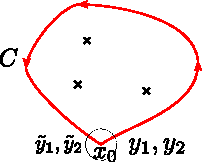
\includegraphics{monodromy.pdf}
  \caption{}
  \label{fig:monodromy}
\end{figure}

しかし、$C$の内側に特異点がある場合には、$\yt_1\ne y_1,\yt_2\ne y_2$となるかもしれません。このような場合でも一致の定理の系\ref{:identity2}から、$\yt_1$も$\yt_2$も微分方程式\eqref{2ode}の解です。したがってこれらは$y_1,y_2$の線形結合で表すことができます。言い換えると、ある$2\times 2$の定数行列$M_C$があって
\begin{align}
  (\yt_1, \yt_2)
  =(y_1, y_2)M_{C}
\end{align}
と書けます。このように、ある経路に関して解析接続してくることによる関数の変換を\strong{モノドロミー}と呼びます。また、その変換の行列$M$を\strong{モノドロミー行列}と呼びます。

図\ref{fig:monodromy2}のように変形してみると分かるように、モノドロミー行列は、$C$の内側にある各特異点のまわりのモノドロミー行列の積に分解出来ます。したがって、\strong{特異点のまわりでの解の構造を調べることが出来れば、微分方程式のモノドロミーの構造が分かります。}
\begin{figure}[htbp]
  \centering
  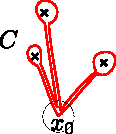
\includegraphics{monodromy2.pdf}
  \caption{}
  \label{fig:monodromy2}
\end{figure}

今分かったのは、微分方程式があると、そのモノドロミーの構造が決まるということです。では、逆にモノドロミーを与えたときに、そのモノドロミーを実現する微分方程式はあるか?という問題を考えることもあります。この種の問題はリーマン・ヒルベルト問題と呼ばれています。

\section{確定特異点}
\subsection{確定特異点とフックスの定理}
ここでは、特異点のうちでも比較的性質の良い\strong{確定特異点}と呼ばれているものを取り扱います。
\begin{definition}{確定特異点}{regularsingularity}
  微分方程式\eqref{2ode}の特異点$x_0$が「確定特異点」である$\Leftrightarrow\ (x-x_0)P(x),\ (x-x_0)^2Q(x)$が$x=x_0$で正則
\end{definition}
これは、言い換えると$P(x)$が高々1位の極、$Q(x)$が高々2位の極ということです。

確定特異点が良い理由は、次のフックスの定理があるからです。
\begin{theor}{フックスの定理}{Fuchstheorem}
  $x=x_0$が微分方程式\eqref{2ode}の確定特異点のとき、
  \begin{align}
    y=(x-x_0)^{\lambda}\sum_{n=0}^{\infty}a_{n}(x-x_0)^{n}\quad (\lambda \text{は定数})
  \end{align}
  の形の解が、少なくとも1つ存在する。
\end{theor}
通常点の場合と異なり、2つ存在するとは限らないことに注意してください。また一般に$\lambda$は複素数ですから、この解は多価関数です。モノドロミーは、$x_0$のまわりを反時計回りに1周まわったとき
\begin{align}
  y\to \exp(2\pi i\lambda) y
\end{align}
となることが、すぐに分かります。

フックスの定理については、次項で詳しく説明します。

\subsection{確定特異点のまわりのべき級数解}
さて、フックスの定理の証明をするために、確定特異点のまわりで、べき級数の方法で微分方程式\eqref{2ode}を調べることにします。

$x=0$が確定特異点であるとします。すると、$P(x)$は$x=0$で高々1位の極、$Q(x)$は高々2位の極ですから
\begin{align}
  P(x)=\sum_{n=-1}^{\infty}p_{n}x^{n},\quad
  Q(x)=\sum_{n=-2}^{\infty}q_{n}x^{n}
\end{align}
とローラン展開できます。$p_n,q_n$は与えられたものであることに注意してください。未知関数$y(x)$を
\begin{align}
  y(x)=x^{\lambda}\sum_{n=0}^{\infty}a_n x^n
\end{align}
と展開できるとしてみます。ここで$a_0\ne 0$としても一般性を失わないので、そうします。$y$の1階、2階の導関数は
\begin{align}
  y'=\sum_{n=0}^{\infty}(\lambda+n)a_nx^{\lambda+n-1},\quad y''=\sum_{n=0}^{\infty}(\lambda+n)(\lambda+n-1) a_n x^{\lambda+n-2}
\end{align}
となることに注意して、微分方程式
\begin{align}
  y''+P(x)y'+Q(x)y=0
\end{align}
に代入してみます。すると
\begin{align}
  \sum_{n=0}^{\infty}(\lambda+n)(\lambda+n-1) a_n x^{\lambda+n-2}+\sum_{m=-1}^{\infty}p_{m}x^{m}\sum_{n=0}^{\infty}(\lambda+n)a_nx^{\lambda+n-1}+\sum_{m=-2}^{\infty}q_{m}x^{m}\sum_{n=0}^{\infty}a_n x^{\lambda+n}=0\nonumber\\
  \Leftrightarrow
  \lambda(\lambda-1)a_0x^{\lambda-2}+\dots
  +(p_{-1}x^{-1}+\dots)(\lambda a_0 x^{\lambda-1}+\dots)+
  (q_{-2}x^{-2}+\dots)(a_0x^{\lambda}+\dots)=0
  \label{tempregularsingularity}
\end{align}
となります。

特に\eqref{tempregularsingularity}の$x^{\lambda-2}$の係数を見てみると$a_0\ne 0$であることを考慮して
\begin{align}
  \lambda(\lambda-1)+p_{-1}\lambda+q_{-2}=0\label{tempdetermining}
\end{align}
という式を得ます。この式から$\lambda$が決定できるので、この方程式のことを\strong{決定方程式}と呼びます。決定方程式の根のことを\strong{特性指数}と呼びます。決定方程式の左辺は、これから良く出てくるので、$\lambda$の2次式$\phi(\lambda)$を
\begin{align}
  \phi(\lambda):=\lambda(\lambda-1)+p_{-1}\lambda+q_{-2}
\end{align}
と定義しておきます。そうすると決定方程式は$\phi(\lambda)=0$と表すことができ、その根は
\begin{align}
  \lambda=\frac12\qty(
    -(p_{-1}-1)\pm \sqrt{(1-p_{-1})^2-4q_{-2}}
  )
\end{align}
となります。この2つの根を$\lambda_{+},\lambda_{-}$としておきます。ただし、$\Re (\lambda_{+}-\lambda_{-})\ge 0$としておきます\footnote{これが成り立っていなかったら、$\lambda_{+}$と$\lambda_{-}$を取り替えてください。}。

次に、式\eqref{tempregularsingularity}の$x^{\lambda+n-2}\ (n=1,2,3,\dots)$の係数を見てみましょう。細かいところを見始めると複雑な式になっていますが、次のような構造をしていることが分かります。
\begin{align}
  (\lambda+n)(\lambda+n-1)a_n+p_{-1}(\lambda+n)a_n+q_{-2}a_n+(a_{k}\ (k<n),\ \lambda\text{の式})=0.
\end{align}
この式の$a_n$が入っている項をよく見ると$\phi(\lambda+n)a_n$となっています。したがって、$\phi(\lambda+n)\ne 0$なら$a_n$について解くことができて
\begin{align}
  a_{n}=\frac{1}{\phi(\lambda+n)}(a_{k}\ (k<n),\ \lambda\text{の式})\qquad \qquad \Atag{n}\label{tempregularsingularity2}
\end{align}
となります。後のために\eqref{tempregularsingularity2}に$\Atag{n}$というラベルをつけました。この場合には、$a_0$を与えると$\Atag{1}$から$a_1$が決まり、$\Atag{2}$から$a_2$が決まり、…というふうになり、すべての$a_n$が決まることになります。

さて、$\phi(\lambda+n)$が$0$になるかどうかを考えましょう。次のことが言えます。
\begin{myquote}
  $\lambda=\lambda_{+}$のとき、$\phi(\lambda_{+}+n)\ne 0\ (n=1,2,3,\dots)$である。
\end{myquote}
証明は次の通りです。$\phi(\lambda_{+}+n)=0$であったと仮定します。$\phi(u)=0$の解は$u=\lambda_{\pm}$のみでしたから、$\lambda_{+}+n=\lambda_{+}$または$\lambda_{+}+n=\lambda_{-}$が成り立ちます。$n=1,2,3,\dots$であることを考えると、前者は明らかに矛盾、後者は$\Re(\lambda_{+}-\lambda_{-})\ge 0$に矛盾します。

これまでの議論で$\lambda=\lambda_{+}$のとき、与えた$a_{0}\ne 0$に対して$a_1,a_2,\dots$が一意に決まることが分かりました。
このとき
\begin{align}
  y=x^{\lambda_{+}}\sum_{n=0}^{\infty}a_{n}x^{n}\label{Fuchssolution1}
\end{align}
は、形式的に\eqref{2ode}の解になります。証明は省略しますが、この無限級数は有限の収束半径をもっています。ここからフックスの定理\ref{:Fuchstheorem}が証明できました。

さて、1つの解は、\eqref{Fuchssolution1}の形で存在することが分かりました。もう1つの解はどうでしょうか。$\lambda=\lambda_{-}$として、上と同じことをやれば、「よほど運が悪くないかぎり」同様に
$a_n$が決まり
\begin{align}
  y=x^{\lambda_{-}}\sum_{n=0}^{\infty}a_{n}x^{n}
  \label{Fuchssolution2}
\end{align}
という形の解が求まります。では、「運が悪い」場合とは、どんな場合でしょうか。次の2つの場合があります。
\begin{itemize}
  \item $\lambda_{+}=\lambda_{-}$の場合。つまり決定方程式が重根を持つ場合です。このとき、\eqref{Fuchssolution2}は、\eqref{Fuchssolution1}と独立ではなくなります。
  \item ある$n\in \{1,2,3,\dots\}$について$\lambda_{-}+n=\lambda_{+}$が成り立つ場合。この場合、\eqref{tempregularsingularity2}のように$a_n$を表すことができなくなり、$a_n$が決まらなくなります。
\end{itemize}
さて、これらの場合にもう1つの解を求めるには、例えば定数変化法を用いれば良いです。もう1つの解を求める別の方法として「フロベニウスの方法」を次項で紹介します。これは、非常に示唆に富んだ方法です。

\subsection{フロベニウスの方法}
ここで、先ほどふれた「運が悪い」場合に、もう1つの解を求める方法を紹介します。
少々天下り的ですが、$\lambda$をもう1つの独立変数として
\begin{align}
  y(x,\lambda):=x^{\lambda}\sum_{n=0}a_n(\lambda)x^{n}
\end{align}
と定義します。ただし、$\lambda$の関数$a_n(\lambda)$は次のように決めます。まず、$a_0(\lambda)$は
\begin{align}
  a_0(\lambda)=
  \begin{cases}
    1& (\lambda_+=\lambda_-)\\
    \lambda-\lambda_{-} & (\lambda_{+}-\lambda_{-}=1,2,3,\dots)
  \end{cases}\label{frobeniuscoefficients}
\end{align}
と決めます。$a_1(\lambda),a_2(\lambda),a_3(\lambda),\dots$は、それぞれ$\Atag{1},\Atag{2},\Atag{3},\dots$から決めます。

ここで導入した$y(x,\lambda)$は一般には式\eqref{2ode}の解ではありません。しかし、ここから次のように独立な2つの解を得ることができます。
\begin{theor}{}{frobenius}
  次の2つは、式\eqref{2ode}の2つの独立な解である。
  \begin{align}
    y_1(x):=y(x,\lambda_{+}),\\
    y_2(x):=\pdv{\lambda}y(x,\lambda)|_{\lambda=\lambda_{-}}.
  \end{align}
\end{theor}

定理\ref{:frobenius}の証明を述べます。$y_1(x)$が解であることは、フックスの定理\ref{:Fuchstheorem}から従います。後は、$y_2(x)$が解であることと、これらが独立であることを示せばよいです。ここでは、$y_2(x)$が解であることの証明を紹介します。独立であることの証明は省略します。

$y(x,\lambda)$が\eqref{2ode}の解ではないのですが、「どれくらい解でないか」を考えてみましょう。$a_n(\lambda)$は式\eqref{tempregularsingularity}のうち、$x^{\lambda-2}$の係数から出てくる条件\eqref{tempdetermining}は満たしていませんが、$x^{\lambda+n-2}\ (n=1,2,3,\dots)$から出てくる条件\eqref{tempregularsingularity2}はすべて満たしています。したがって
\begin{align}
  \qty(
    \pdv[2]{x}+P(x)\pdv{x}+Q(x)
  )y(x,\lambda)=\phi(\lambda)a_0(\lambda)x^{\lambda-2}\label{tempfrobenius}
\end{align}
となります。$\phi(\lambda)=(\lambda-\lambda_{+})(\lambda-\lambda_{-})$であることを思い出すと\eqref{tempfrobenius}の右辺の$\phi(\lambda)a_0(\lambda)$は$(\lambda-\lambda_{-})^2$を因子に持ちます。これは、$a_0(\lambda)$の決め方\eqref{frobeniuscoefficients}から分かります。
したがって
\begin{align}
  \phi(\lambda)a_0(\lambda)=(\lambda-\lambda_{-})^2f(\lambda)
\end{align}
と書いておくことにしましょう。$f(\lambda)=1$または、$f(\lambda)=\lambda-\lambda_{+}$です。

さて、\eqref{tempfrobenius}の両辺に$\pdv{\lambda}$を作用させ、$\lambda=\lambda_{-}$とおくことにします。\eqref{tempfrobenius}の左辺の$()$の中の演算子は$\lambda$によらないことを思い出すと、
\begin{align}
  (\text{左辺})=y_2''(x)+P(x)y_2'(x)+Q(x)y_2(x)
\end{align}
となります。一方、右辺は
\begin{align}
  (\text{右辺})=\pdv{\lambda}
  (
    (\lambda-\lambda_{-})^2 f(\lambda)x^{\lambda-2}
  )\Big|_{\lambda=\lambda_{-}}
  =0
\end{align}
となります。したがって、$y_2(x)$が\eqref{2ode}の解であることが示されました。

フロベニウスの方法は、単に解を求める技術というだけでなく、複素関数論のアイデアを生かした、非常に示唆に富んだ方法です。複素関数論では、単に一点一点での値を考えるのではなく、領域での関数の振る舞いを考えるというのがミソでした。例えば極での関数の値である「未定義」あるいは「$\infty$」だけを見ていても何も情報は得られません。しかし、極を含む領域を考えることで、ローラン展開などをすることによって極の個性が見えてくることになります。同じように$\lambda$は、もともとは決定方程式の解を代入することしか考えていませんでした。そのままでは、$0$で割り算したりすることになってしまった場合、「$a_n$は決まらない」ということしか得られなかったのが問題だったわけです。フロベニウスの方法では、$\lambda$を決定方程式の解だけでなく、それを含む領域で考えることによって、新たな情報を引き出してくることに成功したのです。

1つ簡単な例をやってみましょう。
\begin{align}
  y''+\frac{1}{x}y'+y=0\label{exfrobenius}
\end{align}
という微分方程式を考えます。$x=0$は確定特異点ですから、この方程式を$x=0$のまわりのべき級数展開の方法で解いてみます。
\begin{align}
  y=x^{\lambda}\sum_{n=0}^{\infty}a_nx^{n}
\end{align}
とおいて\eqref{exfrobenius}に代入します。すると
\begin{align}
  \sum_{n=0}^{\infty}(\lambda+n)(\lambda+n-1)a_n x^{\lambda+n-2}
  +\frac{1}{x}\sum_{n=0}^{\infty}(\lambda+n)a_nx^{\lambda+n-1}
  +\sum_{n=0}^{\infty}a_{n}x^{\lambda+n}=0
\end{align}
となります。最後の項だけ$x$のべきが合っていないので、$n$をとりなおして合わせると
\begin{align}
  \sum_{n=0}^{\infty}(\lambda+n)(\lambda+n-1)a_n x^{\lambda+n-2}
  +\sum_{n=0}^{\infty}(\lambda+n)a_n x^{\lambda+n-2}
  +\sum_{n=2}^{\infty}a_{n-2}x^{\lambda+n-2}=0
\end{align}
となります。これを順に見ていきます。

$n=0$のとき、つまり$x^{\lambda-2}$の係数を調べると
\begin{align}
  \phi(\lambda):=\lambda(\lambda-1)+\lambda=\lambda^2
\end{align}
として
\begin{align}
  \phi(\lambda)=0
\end{align}
が出ます。これは$\lambda=0$が重根です。ですから2つめの解を求めるのは一筋縄ではいかないのでフロベニウスの方法を用いることにします。そのために、$y(x,\lambda)$を求めにいくことにします。

$n=1$のとき、つまり$x^{\lambda-1}$の係数を調べると
\begin{align}
  \phi(\lambda+1) a_1=0
  \ \Rightarrow\ 
  a_1=0
\end{align}
となります。

$n=2,3,4,\dots$のとき、つまり$x^{\lambda+n-2}\ (n=2,3,4,\dots)$の係数を調べると
\begin{align}
  \phi(\lambda+n)a_n+a_{n-2}=0
\end{align}
となるので、これを$a_n$について解いて
\begin{align}
  a_n(\lambda)=-\frac{1}{(\lambda+n)^2}a_{n-2}
\end{align}
を得ます。ですから$a_0=1$として
\begin{align}
  a_{\text{奇数}}(\lambda)=0,\quad
  a_{2k}(\lambda)=\prod_{\ell=1}^{k}\frac{-1}{(\lambda+2\ell)^2}
\end{align}
と解けます。この$a_n$を用いて$y(x,\lambda)$は
\begin{align}
  y(x,\lambda)=\sum_{n=0}^{\infty}a_n(\lambda)x^{\lambda+n}
\end{align}
と書けます。
1つめの解は
\begin{align}
  y_1(x)=y(x,\lambda=0)=\sum_{k=0}^{\infty}
  \qty(\prod_{\ell=1}^{k}\frac{-1}{(2\ell)^2}) x^{2k}\label{exfrobeniussolution1}
\end{align}
となります。もう1つの解は
\begin{align}
  y_{2}(x)=\pdv{\lambda} y(x,\lambda)
  |_{\lambda=0}
  =\sum_{k=0}^{\infty}\pdv{\lambda} a_{2k}(\lambda) 
  |_{\lambda=0}x^{2k}
  +\sum_{k=0}^{\infty}a_{2k}(0) (\log x) x^{2k}
\end{align}
です。第2項目は$(\log x) y_1(x)$です。第1項目を詳しく計算してみましょう。積で表されたものを微分するので、$\log$をとってから微分すると見通しが良いです。$n=2k$のとき
\begin{align}
  \log a_{2k}(\lambda)=\sum_{m=1}^{k}(\log(-1)-2\log (\lambda+2m))
\end{align}
ですから、
\begin{align}
  \frac{1}{a_{2k}}\pdv{\lambda}a_{2k}=
  \pdv{\lambda} \log a_{2k}
  =-\sum_{m=1}^{k}\frac{2}{\lambda+2m}
\end{align}
となります。したがって
\begin{align}
  \pdv{\lambda} a_{2k}(\lambda)|_{\lambda=0}
  =-a_{2k}(0)\sum_{m=1}^{k}\frac{1}{m}
  =-\qty(\prod_{\ell=1}^{k}\frac{-1}{(2\ell)^2})\sum_{m=1}^{k}\frac{1}{m}
\end{align}
となります。合わせると
\begin{align}
  y_2(x)=(\log x) y_1(x)-\sum_{k=0}^{\infty}
  \qty(\prod_{\ell=1}^{k}\frac{-1}{(2\ell)^2})\sum_{m=1}^{k}\frac{1}{m} x^{2k}\label{exfrobeniussolution2}
\end{align}
を得ます。

この例での特異点$x=0$まわりでのモノドロミーを見てみましょう。$y_1,y_2$を原点まわりを反時計回りに1周まわしてきたものをそれぞれ$\yt_1,\yt_2$とします。解の形\eqref{exfrobeniussolution1}、\eqref{exfrobeniussolution2}を見ると\eqref{exfrobeniussolution2}の中の$\log x$のところだけがモノドロミーに寄与します。行列で書くと
\begin{align}
  (\yt_1,\yt_2)=
  (y_1,y_2)\mqty(1&2\pi i\\
  0 & 1)
\end{align}
となります。

\section{超幾何関数と合流型超幾何関数}
\subsection{無限での確定特異点}
複素関数論を勉強したときに複素平面$\Cb$上ではなく、リーマン球面$\CP^1$上で考えると、いろいろ見通しがよくなるということがありました。ここでは、微分方程式\eqref{2ode}を$\CP^1$上で考えることにしましょう。

まずは、$\infty$に関して「確定特異点」という概念を定義する必要があります。このためには、$\infty$を取り扱う常套手段として、独立変数を$w=\frac{1}{x}$と変換して、$w=0$について考えます。この変換で\eqref{2ode}は
\begin{align}
  \dv[2]{y}{w}+\qty(\frac{2}{w}-\frac{1}{w^2}P(\frac{1}{w}))\dv{y}{w}+\frac{1}{w^4}Q(\frac{1}{w})y=0\label{2ode1/w}
\end{align}
と書き直すことができます。ですから、
\begin{definition}{}{}
  \eqref{2ode}で$x=\infty$が確定特異点$\underset{\text{def}}{\Leftrightarrow}$
  \eqref{2ode1/w}で$w=0$が確定特異点
\end{definition}
とすることにします。確定特異点の定義\ref{:regularsingularity}と合わせると、$x=\infty$が確定特異点とは$w\qty(\frac{2}{w}-\frac{1}{w^2}P(\frac{1}{w})),\ w^2\frac{1}{w^4}Q(\frac{1}{w})$がともに$w=0$で正則ということになります。つまり
\begin{important}
  \eqref{2ode}で$x=\infty$が確定特異点$\Leftrightarrow$\ $xP(x),\ x^2 Q(x)$が$x=\infty$で正則
\end{important}
ということになります。この定義を採用すれば、$x=\infty$のまわりでのフックスの定理が成り立ちます。
\begin{theor}{}{}
  \eqref{2ode}で$x=\infty$が確定特異点なら
  \begin{align}
    y=\frac{1}{x^{\lambda}}\sum_{n=0}^{\infty} a_nx^{-n}
  \end{align}
  の形の解を持つ。
\end{theor}

ちなみに、もし$P(x)$あるいは$Q(x)$が$0$でない定数であったとすると、$x=\infty$は確定特異点ではなくなります。

\subsection{フックス型の微分方程式}
これまで、特異点の中でも確定特異点は比較的取り扱いやすいということを見てきました。ですから、確定特異点ではない特異点(不確定特異点と呼びます)が現れないような微分方程式のクラスを考えることは、筋がよいと思われます。これを定義しましょう。
\begin{definition}{フックス型の微分方程式}{}
  \eqref{2ode}が$\CP^1$上で不確定特異点を持たないとき、\eqref{2ode}は\strong{フックス型の微分方程式}であるという。
\end{definition}
特に、フックス型の微分方程式の場合、$\CP^1$上で$P(x),\ Q(x)$の特異点は極のみですから、リウビルの定理の系\ref{:meromorphic}より、$P(x),\ Q(x)$は有理関数になります。


フックス型の微分方程式について、確定特異点の数が少ない順に調べていきましょう。
\begin{itemize}
  \item 確定特異点が$0$個の場合。こういう場合があるのかどうかよく分かりません。
  \item 確定特異点が$1$個の場合。$\infty$を確定特異点として、$P(x)=Q(x)=0$の場合のみです。このとき微分方程式は$y''=0$で、独立な2つの解は$y=x$と$y=1$です。これは新しいものではありません。
  \item 確定特異点が$2$個の場合。メビウス変換で2つの確定特異点を$0$と$\infty$に持ってくることができます。このとき
  \begin{align}
    P(x)=\frac{p_{-1}}{x},\quad Q(x)=\frac{q_{-2}}{x^2}
  \end{align}
  となります。したがって微分方程式\eqref{2ode}は
  \begin{align}
    y''+\frac{p_{-1}}{x}y'+\frac{q_{-2}}{x^2}y=0
  \end{align}
  となります。$y=x^{\lambda}$とおいてみると
  \begin{align}
    \lambda(\lambda-1)+p_{-1}\lambda+q_{-2}=0
  \end{align}
  という決定方程式が得られます。決定方程式の根$\lambda=\lambda_{\pm}$が異なれば、2つの独立な解$x^{\lambda_{\pm}}$が得られます。重根の場合は、定数変化法やフロベニウスの方法を用いると$\log x$を含む解が得られます。どちらにしろ、これらは新しい関数ではありません。ただし、ここから得られる教訓は、フックス型の微分方程式の解は$x^{\lambda}$のような冪関数を難しくしたようなものだということです。
  \item 確定特異点が3個の場合。一般に超幾何関数と呼ばれる新しい関数が解になります。これについては次節で詳しく見ていきます。
\end{itemize}

\subsection{超幾何微分方程式と超幾何関数}
確定特異点が3つの場合のフックス型の微分方程式について調べていきましょう。

まず、メビウス変換をすることで、特異点を$0,1,\infty$に持ってくることができます。そうすると$P(x),\ Q(x)$は、$\Cb$上で$0,1$以外では正則な有理関数ということになります。

さらに$0,1,\infty$が確定特異点ですから
\begin{itemize}
  \item $xP(x),\ x^2 Q(x)$が$x=0,\infty$で正則。
  \item $(x-1)P(x),\ (x-1)^2Q(x)$が$x=1$で正則。
\end{itemize}
という条件を考慮すると
\begin{align}
  P(x)=\frac{m_0+m_1 x}{x(1-x)},\quad
  Q(x)=\frac{n_0+n_1x+n_2 x^2}{x^2(1-x)^2}
  \qquad (m_0,m_1,n_0,n_1,n_2 \text{ は定数})\label{generic01infty}
\end{align}
と書くことができます。

さらに従属変数の変換$y\to x^{\alpha}(1-x)^{\beta}y$を考えます。ここで$\alpha,\beta$を適当に選ぶことにより、\eqref{generic01infty}で$n_0=0,\ n_2=-n_1$とすることができます。また、$m_0=c,\ m_1=-(a+b+1),\ n_1=-ab$と書き直して最終的に
\begin{important}
  \begin{align}
    y''+\frac{c-(a+b+1)x}{x(1-x)}y'-\frac{ab}{x(1-x)}y=0\label{hgde}
  \end{align}    
\end{important}
という微分方程式になります。これを\strong{(ガウスの)超幾何微分方程式}と呼びます。

微分方程式\eqref{hgde}を$x=0$まわりで、べき級数の方法で解くことを考えましょう。前節の方法に従うと、決定方程式の解は
\begin{align}
  \lambda=0,1-c
\end{align}
となります。この$c$が$0$以下の整数でないとき、$\lambda=0$の方の解が存在します。$a_0=1$としたときの、この解を$y=\HG(a,b,c;x)$と書きます。あらわな表式は
\begin{important}
  \begin{align}
    \HG(a,b,c;x)=\sum_{n=0}^{\infty}\frac{(a)_n(b)_n}{(c)_n n!} x^n\label{hgf}
  \end{align}
\end{important}
となります。これ(とこれを解析接続したもの)を\strong{(ガウスの)超幾何関数}と呼びます。ただしここで\strong{ポッホハマー記号}
\begin{align}
  (a)_n:=a(a+1)\dots (a+n-1)=\frac{\Gamma(a+n)}{\Gamma(a)}
\end{align}
を導入しました。

表示\eqref{hgf}は$|x|<1$で絶対収束し、$x$に関する正則関数になります。一般に$x=1$は分岐点になっていて、多価関数になります。カットを入れて一価関数にするときは、実軸上$x\ge 1$のところにカットをいれることが多いです。

一般の$a,b,c$に関しては、$\HG(a,b,c;x)$は新しい関数になります。しかし、特殊な$a,b,c$の値に関しては、よく知っている関数になります。この例をいくつか見てみましょう。例えば
\begin{align}
  \HG(a,b,b;x)=\sum_{n=0}^{\infty}\frac{(a)_n(b)_n}{(b)_n n!}x^n=\sum_{n=0}^{\infty}\frac{(a)_n}{n!}x^n
  =(1-x)^{-a}
\end{align}
となります。ここから得られる直感は、超幾何関数はべき関数$(1-x)^{-a}$を難しくしたものということです。別の例は
\begin{align}
  \HG(1,1,2;x)=\sum_{n=0}^{\infty}\frac{(1)_n(1)_n}{(2)_n n!}x^n=\sum_{n=0}^{\infty}\frac{1}{n+1}x^n=-\frac{1}{x}\log(1-x)
\end{align}
です。超幾何関数は$\log$を難しくしたものということもできます。

\subsection{超幾何関数の積分表示}
超幾何関数に関する公式はたくさんあるのですが、ここではその中から積分表示を紹介します。

$|x|<1$での超幾何関数の表式\eqref{hgf}は、ガンマ関数を用いて
\begin{align}
  \HG(a,b,c;x)=\sum_{n=0}^{\infty}\frac{(a)_n(b)_n}{(c)_n n!} x^n
  =\frac{\Gamma(c)}{\Gamma(a)\Gamma(b)}
  \sum_{n=0}^{\infty}\frac{\Gamma(a+n)\Gamma(b+n)}{\Gamma(c+n)n!}x^n\label{temphggamma}
\end{align}
と書けることに注目します。

天下り的ですが、次のような積分を考えます。
\begin{align}
  I=\int_{0}^{1}\dd{t}t^{a-1}(1-t)^{c-a-1}(1-tx)^{-b}.
  \label{temphgintegral}
\end{align}
ただし、カットの入れ方は、図\ref{fig:hgcut}のようにし、$0<t<1$で$\log t=\ln t,\ \log(1-t)=\ln(1-t)$そして$(1-tx)^{-b}$が$t=0$のまわりでテイラー展開した表式となるブランチをとります。この積分は$\Re a>0,\ \Re(c-a)>0$で収束します。
これは、$x=0$のときはベータ関数になる積分でした。つまり、ベータ関数に出てきた積分をちょっとだけ難しくした積分を考えようというわけです。
\begin{figure}[htbp]
  \centering
  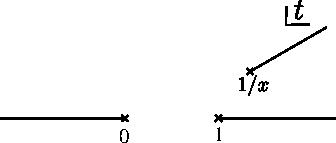
\includegraphics{hgcut.pdf}
  \caption{}
  \label{fig:hgcut}
\end{figure}


$(1-tx)^{-b}$という部分に注目します。$0<t<1,\ |x|<1$ですから、テイラー展開すると次のように一様収束するべき級数の和に書き換えられます。
\begin{align}
  (1-tx)^{-b}=\sum_{n=0}^{\infty}\frac{(-b)(-b-1)\dots (-b-n+1)}{n!}(-tx)^n
  =\sum_{n=0}^{\infty}\frac{(b)_n}{n!}t^nx^n
  =\sum_{n=0}^{\infty}\frac{\Gamma(b+n)}{\Gamma(b)n!}t^n x^n.
\end{align}

これを\eqref{temphgintegral}に代入して和と積分を入れ替えて計算していきます。
\begin{align}
  I&=
  \sum_{n=0}^{\infty}\frac{\Gamma(b+n)}{\Gamma(b)n!} x^n
  \int_{0}^{1}\dd{t}t^{a+n-1}(1-t)^{c-a-1}
  =\sum_{n=0}^{\infty}\frac{\Gamma(b+n)}{\Gamma(b)n!} x^n
  B(a+n,c-a)\nonumber\\
  &=\frac{\Gamma(c-a)}{\Gamma(b)}\sum_{n=0}^{\infty}\frac{\Gamma(a+n)\Gamma(b+n)}{\Gamma(c+n)n!} x^n
\end{align}
となります。途中ベータ関数の定義や公式を使いました。これを\eqref{temphggamma}と比較すると
\begin{align}
  I=\frac{\Gamma(c-a)\Gamma(a)}{\Gamma(c)}\HG(a,b,c;x)
  =B(a,c-a)\HG(a,b,c;x)
\end{align}
となります。ここから、超幾何関数の積分表示
\begin{important}
  \begin{align}
    \HG(a,b,c;x)=\frac{1}{B(a,c-a)}\int_{0}^{1}\dd{t}t^{a-1}(1-t)^{c-a-1}(1-tx)^{-b}
  \end{align}    
\end{important}
を得ます。

この積分表示を見ると、やはり冪関数を難しくしたものと言うことができます。

\subsection{合流型超幾何微分方程式と合流型超幾何関数}
天下り的ですが、次の形の微分方程式を\strong{合流型超幾何微分方程式}と呼びます。
\begin{important}
  \begin{align}
    y''+\qty(\frac{c}{x}-1)y'-\frac{a}{x}y=0,\quad (a,c:\text{ 定数}).\label{chgde}
  \end{align}
\end{important}

まず、\eqref{chgde}の特異点について考えましょう。特異点は$x=0$と$x=\infty$の2つです。$x=0$は確定特異点です。一方で$x=\infty$は不確定特異点です。ただし、$P(x),Q(x)$は$x=\infty$で正則なので、不確定特異点の中でも比較的ましなやつです。このような不確定特異点を1級の不確定特異点と呼んだりします。

次に合流型超幾何微分方程式の名前の由来についてお話します。図\ref{fig:confluent}を見てください。左側は確定特異点が3つある、超幾何微分方程式です。ここでパラメータを動かして3つの特異点のうち2つを「合流」させることを考えます。そうすると右側のように合流した特異点は不確定特異点になります。それ以外の1つの特異点は確定特異点になります。これが合流型超幾何微分方程式です。
\begin{figure}[htbp]
  \centering
  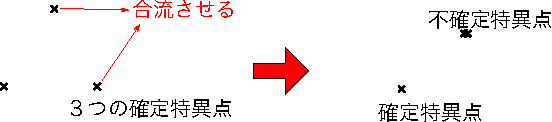
\includegraphics{confluent.pdf}
  \caption{}
  \label{fig:confluent}
\end{figure}

この合流という操作を式で説明します。まず、超幾何微分方程式から始めます。
\begin{align}
  y''+\frac{c-(a+b+1)x}{x(1-x)}y'-\frac{ab}{x(1-x)}y=0.
\end{align}
この微分方程式の$x=1$にある特異点を$x=\infty$にある特異点に合流させることを考えます。そのために、独立変数を$w=bx$に変換します。すると、
\begin{align}
  \dv[2]{y}{w}+\frac{c-(a+1)\frac{w}{b}-w}{w(1-\frac{w}{b})}\dv{y}{w}-\frac{a}{w(1-\frac{w}{b})}y=0
\end{align}
となります。この方程式では、$w=0,b,\infty$に確定特異点があります。$b\to \infty$の極限をとると$w=b$の特異点と$w=\infty$の特異点が合流します。そうすると
\begin{align}
  \dv[2]{y}{w}+\frac{c-w}{w}\dv{y}{w}-\frac{a}{w}y=0
\end{align}
を得ます。これは、合流型超幾何微分方程式\eqref{chgde}に他なりません。

合流型超幾何微分方程式の$x=0$のまわりでの解を考えます。一般的な$a,c$の値に対して$y(0)=1$を満たす解を$y=\CH(a,c;x)$と書くと、この具体的な形は
\begin{important}
  \begin{align}
    \CH(a,c;x)=\sum_{n=0}^{\infty}\frac{(a)_n}{(c)_n n!}x^n
    \label{chgf}
  \end{align}    
\end{important}
となります。これを\strong{合流型超幾何関数}と呼びます。

$\CH(a,c;x)$は一般の$a,c$に対して新しい関数です。特殊な$a,c$の値に対しては、知っている関数になることがあります。例えば
\begin{align}
  \CH(a,a;x)=\sum_{n=0}^{\infty}\frac{(a)_n}{(a)_n n!}x^n
  =\sum_{n=0}^{\infty}\frac{1}{n!}x^n=e^x
\end{align}
となります。ここから得られる直感は、合流型超幾何関数は、指数関数を難しくしたものということです。

\subsection{合流型超幾何関数の積分表示}
合流型超幾何関数にも超幾何関数のような積分表示があります。これを導いてみましょう。

まず、式\eqref{chgf}をガンマ関数を用いて書いておきましょう。
\begin{align}
  \CH(a,c;x)=\frac{\Gamma(c)}{\Gamma(a)}\sum_{n=0}^{\infty}
  \frac{\Gamma(a+n)}{\Gamma(c+n)n!}x^n.
\end{align}

また天下り的ですが、次の積分を考えます。
\begin{align}
  I=\int_{0}^{1}\dd{t}t^{a-1}(1-t)^{c-a-1}e^{xt}.
\end{align}
これは、$\Re a>0,\ \Re(c-a)>0$で収束します。この$I$を計算していきます。指数関数のテイラー展開は収束半径$\infty$ですから、積分と和の順序を交換してよくて
\begin{align}
  I
  =\int_{0}^{1}\dd{t}t^{a-1}(1-t)^{c-a-1}e^{xt}
  =\int_{0}^{1}\dd{t}t^{a-1}(1-t)^{c-a-1}\sum_{n=0}^{\infty}\frac{1}{n!}(xt)^n\nonumber\\
  =\sum_{n=0}^{\infty}\frac{1}{n!} x^n\int_{0}^{1}\dd{t}t^{a+n-1}(1-t)^{c-a-1}
  =\sum_{n=0}^{\infty}\frac{\Gamma(a+n)\Gamma(c-a)}{\Gamma(c+n)n!} x^n\nonumber\\
  =B(a,c-a)\CH(a,c;x)
\end{align}
と計算できます。途中ベータ関数の定義や、ガンマ関数との関係などを用いました。
ここから合流型超幾何関数の積分表示
\begin{important}
  \begin{align}
    \CH(a,c;x)=\frac{1}{B(a,c-a)}\int_{0}^{1}\dd{t}t^{a-1}(1-t)^{c-a-1}e^{xt}
  \end{align}
\end{important}
を得ます。

この積分表示を見ると、やはり合流型超幾何関数は$e^x$を難しくしたものだと思うことができます。

\subsection{物理に現れる特殊関数}
実は、超幾何関数と合流型超幾何関数は、物理によく現れるかなり広いクラスの特殊関数の親玉みたいなものです。

例えば、ルジャンドル関数(多項式、陪関数)は超幾何関数です。実際ルジャンドル関数の満たす微分方程式
\begin{align}
  (1-x^2)y''-2x y'+[\ell(\ell+1)-\frac{m^2}{1-x^2}]y=0
\end{align}
の特異点は$x=-1,+1,\infty$の3つで、すべて確定特異点です。

他には、ラゲール関数(多項式、陪多項式)、エルミート関数(多項式)、ベッセル関数は合流型超幾何関数です。量子力学の教科書を見て、確認してみてください。

みなさんが今後物理を勉強、研究する上で新しい微分方程式に出会うかもしれません。その微分方程式が2階の線形微分方程式なら、解はそれなりに高い確率で超幾何関数か合流型超幾何関数です。それを見極めるには、特異点に注目すればよいです。
\begin{itemize}
  \item 特異点が3つ(以下)で、すべて確定特異点の場合、解は超幾何関数です。
  \item 特異点が2つで、一方が確定特異点、もう一方が1級不確定特異点の場合、解は合流型超幾何関数です。
  \item それ以外の場合は、変数変換などをがんばってみると上のどちらかになるかも知れません。それが無理なら別のクラスの関数になります。
\end{itemize}

\section{まとめ}
この章では、2階の線形微分方程式に注目し、その性質を調べました。
\begin{itemize}
  \item 通常点のまわりでは、正則で独立な2つの解が存在します。
  \item 特異点のまわりを調べることが重要です。
  \item 確定特異点という、扱いやすい特異点があります。確定特異点のまわりでは、べき級数の解が、少なくとも1つ存在します。
  \item もう1つの解が素朴な方法で求まらない場合には、フロベニウスの方法という、示唆に富んだ方法があります。
  \item 超幾何関数、合流型超幾何関数という、特殊関数の親玉みたいな関数があります。
\end{itemize}


\chapter{ベッセル関数}
\section{生成母関数}
ベッセル関数の導入の仕方は、いろんなやり方があります。ここでは、生成母関数から導入しましょう。$t$と$x$の関数
\begin{align}
  e^{\frac{x}{2}\qty(t-\frac{1}{t})}
\end{align}
を考えます。この関数で$t=0$は真性特異点です。$t=0$のまわりでローラン展開することを考えましょう。
\begin{important}
  \begin{align}
    e^{\frac{x}{2}\qty(t-\frac{1}{t})}=\sum_{n=-\infty}^{\infty}
    J_n(x)t^{n}.\label{generatingBessel1}
  \end{align}  
\end{important}
このときに$t^n$の係数に現れる$x$の関数$J_n(x), \ n\in \Zb$を\strong{第1種ベッセル関数}と呼びます。

さて、具体的にローラン展開を実行して$J_n(x)$の形を求めてみましょう。
\begin{align}
  e^{\frac{x}{2}\qty(t-\frac{1}{t})}=e^{\frac{xt}{2}}e^{-\frac{x}{2t}}
  =\sum_{k=0}^{\infty}\frac{1}{k!}\qty(\frac{xt}{2})^k
  \sum_{\ell=0}^{\infty}\frac{1}{\ell !}\qty(\frac{-x}{2t})^{\ell}
  =\sum_{k=0}^{\infty}\sum_{\ell=0}^{\infty}\frac{(-1)^{\ell}}{k!\ell !}t^{k-\ell}\qty(\frac{x}{2})^{k+\ell}.
\end{align}
ここで$n=k-\ell$とおいて、和の変数の1つの$k$を$n$に変換します。
\begin{align}
  e^{\frac{x}{2}\qty(t-\frac{1}{t})}=\sum_{n=-\infty}^{\infty}
  \sum_{\ell=0}^{\infty}\frac{(-1)^{\ell}}{(n+\ell)!\ell !}\qty(\frac{x}{2})^{n+2\ell}
  t^{n}
\end{align}
という形を得ます。ただし、$m$を負の整数としたとき$1/m!=1/\Gamma(m+1)=0$としています。ここから第1種ベッセル関数が
\begin{important}
  \begin{align}
    J_n(x)=\sum_{\ell=0}^{\infty}\frac{(-1)^{\ell}}{(n+\ell)!\ell !}\qty(\frac{x}{2})^{n+2\ell}\label{defBessel1int}
  \end{align}
\end{important}
と求まります。

ここまでは、整数$n$に対して$J_n(x)$を定義しました。次にこれを拡張し、複素数$\nu$に対して$J_{\nu}(x)$を定義することを考えましょう。式\eqref{defBessel1int}の中で、単に$n$を$\nu$で置き換えることを考えます。階乗は一般化したガンマ関数に置き換えることができますし、べき関数も多価関数になることを厭わなければ、置き換えることができます。これをもって$J_{\nu}(x)$の定義としましょう。
\begin{important}
  \begin{align}
    J_{\nu}(x):=\sum_{\ell=0}^{\infty}\frac{(-1)^{\ell}}{\Gamma(\nu+\ell+1)\ell !}\qty(\frac{x}{2})^{\nu+2\ell}.\label{defBessel1}
  \end{align}
\end{important}
こうして拡張したものも\strong{第1種ベッセル関数}と呼びます。

第1種ベッセル関数に関して少し直感を得るために、$\nu=\frac12$の場合を考えてみます。ガンマ関数の関係式
\begin{align}
  \Gamma\qty(\frac12+\ell+1)=\qty(\ell+\frac12)\qty(\ell-\frac12)\dots \frac12 \Gamma\qty(\frac12)
\end{align}
から
\begin{align}
  \Gamma\qty(\frac12+\ell+1)\ell!=\qty(\ell+\frac12)\ell\qty(\ell-\frac12)(\ell-1)\dots 1\cdot\frac12 \sqrt{\pi}
  =\frac{(2\ell+1)!\sqrt{\pi}}{2^{2\ell+1}}
\end{align}
という関係が成り立ちます。これを用いて$\nu=\frac12$の場合に\eqref{defBessel1}を考えると
\begin{align}
  J_{\frac12}(x)
  &=\sum_{\ell=0}^{\infty}\frac{(-1)^{\ell}}{\Gamma\qty(\frac12+\ell+1)\ell !}\qty(\frac{x}{2})^{\frac12+2\ell}
  =\sqrt{\frac{2}{x}}\sum_{\ell=0}^{\infty}\frac{(-1)^{\ell}2^{2\ell+1}}{(2\ell+1)!\sqrt{\pi}}\qty(\frac{x}{2})^{2\ell+1}\nonumber\\
  &=\sqrt{\frac{2}{\pi x}}\sum_{\ell=0}^{\infty}\frac{(-1)^{\ell}}{(2\ell+1)!}x^{2\ell+1}
  =\sqrt{\frac{2}{\pi x}}\sin x
\end{align}
となります。ここから得られる直感は、第1種ベッセル関数は三角関数を難しくしたもの、ということです。

\section{積分表示}
これまで取り扱ってきた様々な特殊関数と同様に、第1種ベッセル関数に関しても積分表示を考えることは役に立ちます。ここでは、いくつかの積分表示を紹介します。

$n$が整数の場合、式\eqref{generatingBessel1}からすぐに
\begin{align}
  J_n(x)=\frac{1}{2\pi i}\oint_{0}\dd{t}t^{-n-1}e^{\frac{x}{2}\qty(t-\frac{1}{t})}\label{bessel1oint}
\end{align}
が従います。ここで積分経路は$t=0$のまわりを反時計回りに回る小さな円です。この積分を$t=e^{i\theta}\ (-\pi\le \theta \le \pi)$とパラメータ表示して評価することにします。
\begin{align}
  J_n(x)
  =\frac{1}{2\pi i}\int_{-\pi}^{\pi}\dd{\theta}
  ie^{-in\theta}e^{\frac{x}{2}(e^{i\theta}-e^{-i\theta})}
  =\frac{1}{2\pi}\int_{-\pi}^{\pi}\dd{\theta}
  e^{-in\theta+ix\sin\theta}
\end{align}
ここで、積分範囲を$-\pi$から$0$と$0$から$\pi$の2つに分け、$-\pi$から$0$の方の積分で$\theta\to -\theta$の変数変換を行うと
\begin{important}
  \begin{align}
    J_n(x)=\frac{1}{\pi}\int_{0}^{\pi}\dd{\theta}
    \cos(n\theta-x\sin\theta)
  \end{align}
\end{important}
という積分表示が得られます。

一般の$\nu$に対する積分表示を考えてみましょう。それを予想するために\eqref{bessel1oint}で積分変数を$t$から$s=\frac{xt}{2}$に変換します。すると
\begin{align}
  J_n(x)=\frac{1}{2\pi i}\qty(\frac{x}{2})^{n}\oint_{0}\dd{s}
  s^{-n-1}e^{s-\frac{x^2}{4s}}\label{tempbessel1}
\end{align}
という表式を得ます。積分経路はまだ図\ref{fig:besselcontour}の(a)のような経路です。これを変形して、図\ref{fig:besselcontour}の(b)のようにします。$\Re s\to -\infty$で被積分関数は十分早く$0$に収束しますから、無限のところでどうなっているかは、気にしなくてもよいです。このような変形をすることにより、\eqref{tempbessel1}の右辺で$n$を一般の複素数$\nu$に変えたものが積分として意味を持ちます。したがって、次のような関係式が予想できます。
\begin{important}
  \begin{align}
    J_{\nu}(x)=\frac{1}{2\pi i}\qty(\frac{x}{2})^{\nu}\int_{C}\dd{s}
    s^{-\nu-1}e^{s-\frac{x^2}{4s}}.
    \label{bessel1intnu}
  \end{align}
\end{important}
ここで、積分経路$C$は図\ref{fig:besselcontour}の(b)の経路です。実軸負の部分にカットを入れ、$s>0$のとき$\log s=\ln s$となるブランチをとっています。
\begin{figure}[htbp]
  \centering
  \begin{tabular}{cc}
   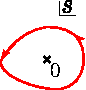
\includegraphics[scale=1.5]{contour0.pdf}&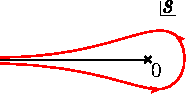
\includegraphics[scale=1.5]{ophankel.pdf}\\
   (a) & (b) 
  \end{tabular}
  \caption{}
  \label{fig:besselcontour}
\end{figure}

\eqref{bessel1intnu}が実際に成り立つことを証明しましょう。右辺の$e^{-\frac{x^2}{4s}}$を展開し、無限和と積分を入れ替えます\footnote{無限和と積分を入れ替えてもよいことは、本当は証明が必要なことです。}。
\begin{align}
  (\text{右辺})=\frac{1}{2\pi i}\qty(\frac{x}{2})^{\nu}\int_{C}\dd{s}
  s^{-\nu-1}e^{s}\sum_{\ell=0}^{\infty}\frac{(-1)^{\ell}}{\ell !} \frac{1}{s^{\ell}}\qty(\frac{x}{2})^{2\ell}
  =\sum_{\ell=0}^{\infty}\frac{(-1)^{\ell}}{\ell !}\qty(\frac{x}{2})^{\nu+2\ell}\frac{1}{2\pi i}\int_{C}\dd{s}
  s^{-\nu-\ell-1}e^{s}.
\end{align}
ここで、$s$に関する積分はハンケルの積分表示のちょっと変わったもので、演習問題第2回でみなさんにやってもらったものです。結果を書くと
\begin{align}
  \frac{1}{2\pi i}\int_{C}\dd{s}
  s^{-\nu-\ell-1}e^{s}=\frac{1}{\pi}\sin(\pi(-\nu-\ell))\Gamma(-\nu-\ell)=\frac{1}{\Gamma(\nu+\ell+1)}
\end{align}
となります。最後の変形では、相補公式\eqref{reflectionformula}を用いました。ここから
\begin{align}
  (\text{右辺})=\sum_{\ell=0}^{\infty}\frac{(-1)^{\ell}}{\Gamma(\nu+\ell+1)\ell !}\qty(\frac{x}{2})^{\nu+2\ell}=J_{\nu}(x)
\end{align}
となり、\eqref{bessel1intnu}が証明されました。

\eqref{bessel1oint}や\eqref{bessel1intnu}からは、他にも様々な積分表示が得られます。興味がある人は公式集などをみてみてください。

\section{漸化式、微分方程式}
ベッセル関数が物理によく出てくる理由は、それがある2階の微分方程式を満たすからです。ここでは、それを見ていきましょう。微分方程式を説明するためには、まず漸化式を導出するのが近道です。ですので、ここでは第1種ベッセル関数が満たす漸化式を導出し、それを用いて微分方程式を導出します。

積分表示\eqref{bessel1intnu}から始めて変形していきます。$\nu\ne 0$のとき$s^{-\nu-1}=-\frac{1}{\nu}\qty(\dv{s}s^{-\nu})$という関係を用いて
\begin{align}
  J_{\nu}(x)
  &=\frac{1}{2\pi i}\qty(\frac{x}{2})^{\nu}\int_{C}\dd{s}(-1)\frac{1}{\nu}\qty(\dv{s}s^{-\nu})
  e^{s-\frac{x^2}{4s}}\nonumber\\
  &=\frac{1}{\nu}\frac{1}{2\pi i}\qty(\frac{x}{2})^{\nu}\int_{C}\dd{s}s^{-\nu}\dv{s}
  e^{s-\frac{x^2}{4s}}
  =\frac{1}{\nu}\frac{1}{2\pi i}\qty(\frac{x}{2})^{\nu}\int_{C}\dd{s}s^{-\nu}\qty(1+\frac{x^2}{4s^2})
  e^{s-\frac{x^2}{4s}}    
\end{align}
となりますので
\begin{align}
  \frac{2\nu}{x}J_{\nu}(x)=\frac{1}{2\pi i}\qty(\frac{x}{2})^{\nu-1}\int_{C}\dd{s}s^{-\nu}
  e^{s-\frac{x^2}{4s}}
  +\frac{1}{2\pi i}\qty(\frac{x}{2})^{\nu+1}\int_{C}\dd{s}s^{-\nu-2}
  e^{s-\frac{x^2}{4s}}
  =J_{\nu-1}(x)+J_{\nu+1}(x)
\end{align}
となります。したがって漸化式
\begin{important}
  \begin{align}
    J_{\nu-1}(x)+J_{\nu+1}(x)=\frac{2\nu}{x}J_{\nu}(x)
    \label{besselrecursion1}
  \end{align}
\end{important}
が得られます。

漸化式はもう1つあります。\eqref{bessel1intnu}の両辺を$x$で微分します。
\begin{align}
  J'_{\nu}(x)=
  \frac{1}{2\pi i}\frac{\nu}{2}\qty(\frac{x}{2})^{\nu-1}\int_{C}\dd{s}s^{-\nu-1}e^{s-\frac{x^2}{4s}}
  +\frac{1}{2\pi i}\qty(\frac{x}{2})^{\nu}\int_{C}\dd{s}s^{-\nu-1}\qty(-\frac{x}{2s})e^{s-\frac{x^2}{4s}}
  =\frac{\nu}{x}J_{\nu}(x)-J_{\nu+1}(x).
\end{align}
右辺の第1項に\eqref{besselrecursion1}を用いると、もう1つの漸化式
\begin{important}
  \begin{align}
    J_{\nu-1}(x)-J_{\nu+1}(x)=2J'_{\nu}(x)\label{besselrecursion2}
  \end{align}
\end{important}
を得ます。

さて、これらから微分方程式を導出しましょう。\eqref{besselrecursion1}と\eqref{besselrecursion2}を足して2で割ったものと引いて2で割ったものを考えると、それぞれ
\begin{align}
  J_{\nu-1}=J'_{\nu}+\frac{\nu}{x}J_{\nu},\label{tempbesselde0}\\
  J_{\nu+1}=-J'_{\nu}+\frac{\nu}{x}J_{\nu}\label{tempbesselde1}
\end{align}
となります。\eqref{tempbesselde1}で$\nu$を$\nu-1$と書くと
\begin{align}
  J_{\nu}=-J'_{\nu-1}+\frac{\nu-1}{x}J_{\nu-1}
\end{align}
となります。これに\eqref{tempbesselde0}を代入すると
\begin{align}
  J_{\nu}=-\qty(J'_{\nu}+\frac{\nu}{x}J_{\nu})'
  +\frac{\nu-1}{x}\qty(J'_{\nu}+\frac{\nu}{x}J_{\nu})
\end{align}
となり、これを整理すると微分方程式
\begin{align}
  J''_{\nu}+\frac{1}{x}J'_{\nu}+\qty(1-\frac{\nu^2}{x^2})J_{\nu}=0
\end{align}
を得ます。つまり
\begin{important}
  $J_{\nu}(x)$は、微分方程式
  \begin{align}
    y''+\frac{1}{x}y'+\qty(1-\frac{\nu^2}{x^2})y=0
    \label{besselde}
  \end{align}
  の1つの解である。
\end{important}
ということが言えます。微分方程式\eqref{besselde}は\strong{ベッセルの微分方程式}と呼ばれます。

ベッセルの微分方程式\eqref{besselde}の特異点を調べてみましょう。特異点は、$x=0$と$x=\infty$です。$x=0$は確定特異点です。$x=\infty$は不確定特異点ですが、1級の不確定特異点です。したがってベッセルの微分方程式\eqref{besselde}は、合流型超幾何微分方程式です。うまく独立変数、従属変数を変数変換することによって\eqref{chgde}の形にもっていくことができます。

ベッセルの微分方程式\eqref{besselde}の1つの解は$J_{\nu}(x)$ですが、もう1つの解は何でしょうか。\eqref{besselde}の中には$\nu$は$\nu^2$の形でしか入っていませんから$J_{-\nu}(x)$も解です。実際$\nu$が整数でないときには、$J_{\nu}(x)$と$J_{-\nu}(x)$が\eqref{besselde}の独立な2つの解になります。

ところが、$\nu=n\in \Zb$の場合には、$J_{n}(x)$と$J_{-n}(x)$が独立ではないことが次のようにして分かります。$n=0$のときには自明です。$n>0$として$1/\Gamma(-n+\ell+1)=0\quad (\ell=0,1,2,\dots,n-1)$であることに注目すると
\begin{align}
  J_{-n}(x)
  &=\sum_{\ell=0}^{\infty}\frac{(-1)^{\ell}}{\Gamma(-n+\ell+1)\ell !}\qty(\frac{x}{2})^{-n+2\ell}
  =\sum_{\ell=n}^{\infty}\frac{(-1)^{\ell}}{\Gamma(-n+\ell+1)\ell !}\qty(\frac{x}{2})^{-n+2\ell}\nonumber\\
  &=\sum_{\ell'=0}^{\infty}\frac{(-1)^{\ell'+n}}{\Gamma(\ell'+1)(\ell'+n) !}\qty(\frac{x}{2})^{n+2\ell'}
  =(-1)^n\sum_{\ell'=0}^{\infty}\frac{(-1)^{\ell'}}{\ell'!(\ell'+n) !}\qty(\frac{x}{2})^{n+2\ell'}\nonumber\\
  &=(-1)^n J_{n}(x)
\end{align}
となります。途中で和を取る変数の変換$\ell=\ell'+n$をしました。実際これは\eqref{besselde}を確定特異点$x=0$のまわりでべき級数の方法で解を見つけようとしたときに、決定方程式の2つの根の差が整数になってしまった場合に対応しています。

$\nu=n\in \Zb$の場合に、もう1つの解を見つけるには、どうすればよいでしょうか。もちろんフロベニウスの方法を用いてもよいです。しかし、よく用いられるもう1つの解は、次のようなものです。$\nu \notin \Zb$の場合に
\begin{important}
  \begin{align}
    Y_{\nu}(x):=\frac{1}{\sin(\pi\nu)}(\cos(\pi\nu)J_{\nu}(x)-J_{-\nu}(x))
  \end{align}
\end{important}
を定義します。整数$n$に対しても
\begin{align}
  Y_n(x):=\lim_{\nu\to n}Y_{\nu}(x)
\end{align}
で定義します。これはちゃんと極限を持ちます。こうすると$\nu$が整数でも整数でなくても$J_{\nu}(x)$と$Y_{\nu}(x)$が\eqref{besselde}の独立な2つの解になります。$Y_{\nu}(x)$のことを\strong{第2種ベッセル関数}と呼びます\footnote{文献によって第2種ベッセル関数のことを$N_{\nu}(x)$という記号であらわしてあるものもあります。}。

\section{ベッセル関数が物理に現れる例}
ここで物理でベッセル関数が現れる例を1つ紹介します。

直交座標$x_1,x_2$で表される平面上を考えます。この平面内で、原点中心の半径$a$の円板内で定義された関数$\psi(x_1,x_2)$を考えます。$\psi(x_1,x_2)$は固定端条件$\psi(x_1,x_2)|_{x_1^2+x_2^2=a^2}=0$を満たすとします。この関数に対するラプラシアン
\begin{align}
  \laplacian=\pdv[2]{x_1}+\pdv[2]{x_2}
\end{align}
の固有値問題
\begin{align}
  -\laplacian \psi(x_1,x_2)=\lambda \psi(x_1,x_2)\label{disklaplaceeigenfunc}
\end{align}
を考えます。

このような問題は、例えば円板内に閉じ込められた粒子のシュレーディンガー方程式だったり、丸い太鼓の振動だったり、円柱の管の中の電磁波を考えたりする場合に現れます。

今の問題には回転対称性があるので、極座標をとって考えるのが便利です。
\begin{align}
  x_1=r\cos \phi,\quad x_2=r\sin\phi
\end{align}
として、ラプラシアンをがんばって計算すると
\begin{align}
  \laplacian=\pdv[2]{r}+\frac{1}{r}\pdv{r}+\frac{1}{r^2}\pdv[2]{\phi}
\end{align}
となります。そうすると偏微分方程式\eqref{disklaplaceeigenfunc}は変数分離できます。$\pdv{\phi}$の固有関数は$e^{in\phi} \ (n\in \Zb)$ですから、固有関数は$R(r)$を$r$だけの関数として
\begin{align}
  \psi=R(r)e^{in\phi}\label{tempbesselseparate}
\end{align}
と書けます。$\psi$は原点でなめらかでなければならないので$R(r)$は条件
\begin{align}
  R(0)=0 \quad (n\ne 0),\qquad R(0)=(\text{有限})\quad (n=0)
  \label{tempcondorigin}
\end{align}
を満たす必要があります。\eqref{tempbesselseparate}を\eqref{disklaplaceeigenfunc}に代入して整理すると$R(r)$に対する常微分方程式
\begin{align}
  R''+\frac{1}{r}R'+\qty(\lambda-\frac{n^2}{r^2})R=0
\end{align}
を得ます。独立変数を$\rho:=\sqrt{\lambda}r$と変換すると、この常微分方程式は
\begin{align}
  \dv[2]{R}{\rho}+\frac{1}{\rho}\dv{R}{\rho}+\qty(1-\frac{n^2}{\rho^2})R=0  \label{tempReq}
\end{align}
となり、ベッセルの微分方程式に帰着しました。

微分方程式\eqref{tempReq}の独立な2つの解は、$J_n(\rho)$と$Y_n(\rho)$です。このうち$Y_n(\rho)$の方は条件\eqref{tempcondorigin}を満たさないので
\begin{align}
  R(r)=J_n(\rho)=J_n(\sqrt{\lambda}r)
\end{align}
が解です。

\begin{figure}[htbp]
  \centering
  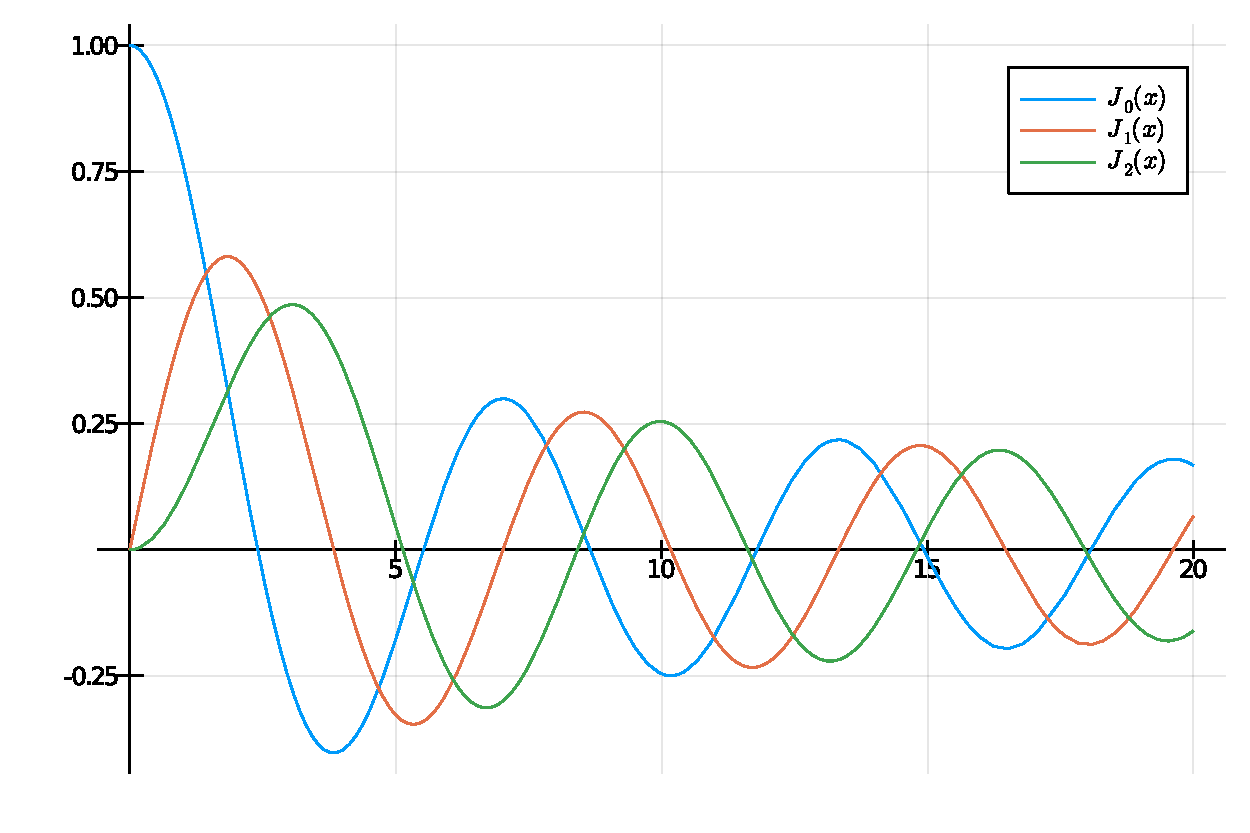
\includegraphics[width=13cm]{besselj2.pdf}
  \caption{$J_n(x)$のグラフ。}
  \label{fig:besselj2}
\end{figure}

さて、円板の端で$0$になるという条件を考えましょう。式で書くなら
\begin{align}
  0=R(a)=J_n(\sqrt{\lambda}a)\label{besselbc}
\end{align}
となります。これを調べるためには、ベッセル関数が0になる点の様子を知っておく必要があります。図\ref{fig:besselj2}には例として$J_n(x)\ (n=0,1,2)$のグラフを示しました。このように$J_n(x)$には$x>0$で無限個の0点が並んでいます。第1種ベッセル関数は三角関数を難しくしたものということを思い出してください。これら$x>0$で$J_n(x)=0$となる点を小さい方から順番に$a_{n,1},a_{n,2},a_{n,3},\dots$とします。そうすると条件\eqref{besselbc}から
\begin{align}
  \lambda=\frac{a_{n,k}^2}{a^2}\qquad (k=1,2,3,4,\dots)
\end{align}
となることが分かり、固有値のスペクトルが得られます。対応する固有関数は
\begin{align}
  \psi=J_n(\frac{a_{n,k}}{a}r)e^{in\phi}
\end{align}
となります。



\section{ハンケル関数、変形ベッセル関数}
最後に少しだけ言葉、記号などを紹介して終わりにしたいと思います。

ベッセルの微分方程式の解の別の基底として次のものが使われることがよくあります。
\begin{important}
  \begin{align}
    H^{(1)}_{\nu}(x):=J_{\nu}(x)+iY_{\nu}(x),\quad
    H^{(2)}_{\nu}(x):=J_{\nu}(x)-iY_{\nu}(x).
  \end{align}    
\end{important}
これらを\strong{ハンケル関数}と呼びます。気持ち的には、$e^{ix},\ e^{-ix}$を難しくしたものです。

次のような関数も文献によく現れます。
\begin{important}
  \begin{align}
    I_{\nu}(x):=e^{-\frac{\pi i \nu}{2}}J_{\nu}(xe^{i\frac{\pi}{2}})
    =\sum_{\ell=0}^{\infty}\frac{1}{\Gamma(\ell+\nu+1)\ell!}\qty(\frac{x}{2})^{\nu+2\ell}.
  \end{align}    
\end{important}
これを\strong{第1種変形ベッセル関数}と呼びます。気持ち的には、双曲線関数を難しくしたものです。定義からすぐに$I_{\nu}(x)$は、次の微分方程式の1つの解であることが分かります。
\begin{important}
  \begin{align}
    y''+\frac{1}{x}y'-\qty(1+\frac{\nu^2}{x^2})y=0.
  \end{align}
\end{important}
この微分方程式は\strong{変形したベッセルの微分方程式}と呼ばれます。もう1つの解として、よく用いられるのは
\begin{important}
  \begin{align}
    K_{\nu}(x)=\frac{\pi}{2}\frac{I_{-\nu}(x)-I_{\nu}(x)}{\sin(\pi\nu)}
  \end{align}
\end{important}
です。これは\strong{第2種変形ベッセル関数}と呼ばれます。

ハンケル関数や変形ベッセル関数に関しても様々な公式があります。公式集をいろいろめくってみると楽しいと思います。

\section{まとめ}
この章では、ベッセル関数について基本的なことの一部をまとめました。
\begin{itemize}
  \item 第1種ベッセル関数$J_{\nu}(x)$を定義しました。
  \item $J_{\nu}(x)$を積分表示する方法をいくつか紹介しました。
  \item $J_{\nu}(x)$は2階の線形微分方程式の解になっています。もう1つの解は第2種ベッセル関数$Y_{\nu}(x)$です。
  \item 物理にベッセル関数が現れる例として、円板内のラプラシアンの固有値問題を紹介しました。
  \item ハンケル関数$H^{(1)}_{\nu}(x),\ H^{(2)}_{\nu}(x)$、変形ベッセル関数$I_{\nu}(x),\ K_{\nu}(x)$もよく現れる関数です。
\end{itemize}

\end{document}
